% Options for packages loaded elsewhere
\PassOptionsToPackage{unicode}{hyperref}
\PassOptionsToPackage{hyphens}{url}
%
\documentclass[
]{book}
\usepackage{amsmath,amssymb}
\usepackage{iftex}
\ifPDFTeX
  \usepackage[T1]{fontenc}
  \usepackage[utf8]{inputenc}
  \usepackage{textcomp} % provide euro and other symbols
\else % if luatex or xetex
  \usepackage{unicode-math} % this also loads fontspec
  \defaultfontfeatures{Scale=MatchLowercase}
  \defaultfontfeatures[\rmfamily]{Ligatures=TeX,Scale=1}
\fi
\usepackage{lmodern}
\ifPDFTeX\else
  % xetex/luatex font selection
\fi
% Use upquote if available, for straight quotes in verbatim environments
\IfFileExists{upquote.sty}{\usepackage{upquote}}{}
\IfFileExists{microtype.sty}{% use microtype if available
  \usepackage[]{microtype}
  \UseMicrotypeSet[protrusion]{basicmath} % disable protrusion for tt fonts
}{}
\makeatletter
\@ifundefined{KOMAClassName}{% if non-KOMA class
  \IfFileExists{parskip.sty}{%
    \usepackage{parskip}
  }{% else
    \setlength{\parindent}{0pt}
    \setlength{\parskip}{6pt plus 2pt minus 1pt}}
}{% if KOMA class
  \KOMAoptions{parskip=half}}
\makeatother
\usepackage{xcolor}
\usepackage[margin=0.79in]{geometry}
\usepackage{color}
\usepackage{fancyvrb}
\newcommand{\VerbBar}{|}
\newcommand{\VERB}{\Verb[commandchars=\\\{\}]}
\DefineVerbatimEnvironment{Highlighting}{Verbatim}{commandchars=\\\{\}}
% Add ',fontsize=\small' for more characters per line
\usepackage{framed}
\definecolor{shadecolor}{RGB}{248,248,248}
\newenvironment{Shaded}{\begin{snugshade}}{\end{snugshade}}
\newcommand{\AlertTok}[1]{\textcolor[rgb]{0.94,0.16,0.16}{#1}}
\newcommand{\AnnotationTok}[1]{\textcolor[rgb]{0.56,0.35,0.01}{\textbf{\textit{#1}}}}
\newcommand{\AttributeTok}[1]{\textcolor[rgb]{0.13,0.29,0.53}{#1}}
\newcommand{\BaseNTok}[1]{\textcolor[rgb]{0.00,0.00,0.81}{#1}}
\newcommand{\BuiltInTok}[1]{#1}
\newcommand{\CharTok}[1]{\textcolor[rgb]{0.31,0.60,0.02}{#1}}
\newcommand{\CommentTok}[1]{\textcolor[rgb]{0.56,0.35,0.01}{\textit{#1}}}
\newcommand{\CommentVarTok}[1]{\textcolor[rgb]{0.56,0.35,0.01}{\textbf{\textit{#1}}}}
\newcommand{\ConstantTok}[1]{\textcolor[rgb]{0.56,0.35,0.01}{#1}}
\newcommand{\ControlFlowTok}[1]{\textcolor[rgb]{0.13,0.29,0.53}{\textbf{#1}}}
\newcommand{\DataTypeTok}[1]{\textcolor[rgb]{0.13,0.29,0.53}{#1}}
\newcommand{\DecValTok}[1]{\textcolor[rgb]{0.00,0.00,0.81}{#1}}
\newcommand{\DocumentationTok}[1]{\textcolor[rgb]{0.56,0.35,0.01}{\textbf{\textit{#1}}}}
\newcommand{\ErrorTok}[1]{\textcolor[rgb]{0.64,0.00,0.00}{\textbf{#1}}}
\newcommand{\ExtensionTok}[1]{#1}
\newcommand{\FloatTok}[1]{\textcolor[rgb]{0.00,0.00,0.81}{#1}}
\newcommand{\FunctionTok}[1]{\textcolor[rgb]{0.13,0.29,0.53}{\textbf{#1}}}
\newcommand{\ImportTok}[1]{#1}
\newcommand{\InformationTok}[1]{\textcolor[rgb]{0.56,0.35,0.01}{\textbf{\textit{#1}}}}
\newcommand{\KeywordTok}[1]{\textcolor[rgb]{0.13,0.29,0.53}{\textbf{#1}}}
\newcommand{\NormalTok}[1]{#1}
\newcommand{\OperatorTok}[1]{\textcolor[rgb]{0.81,0.36,0.00}{\textbf{#1}}}
\newcommand{\OtherTok}[1]{\textcolor[rgb]{0.56,0.35,0.01}{#1}}
\newcommand{\PreprocessorTok}[1]{\textcolor[rgb]{0.56,0.35,0.01}{\textit{#1}}}
\newcommand{\RegionMarkerTok}[1]{#1}
\newcommand{\SpecialCharTok}[1]{\textcolor[rgb]{0.81,0.36,0.00}{\textbf{#1}}}
\newcommand{\SpecialStringTok}[1]{\textcolor[rgb]{0.31,0.60,0.02}{#1}}
\newcommand{\StringTok}[1]{\textcolor[rgb]{0.31,0.60,0.02}{#1}}
\newcommand{\VariableTok}[1]{\textcolor[rgb]{0.00,0.00,0.00}{#1}}
\newcommand{\VerbatimStringTok}[1]{\textcolor[rgb]{0.31,0.60,0.02}{#1}}
\newcommand{\WarningTok}[1]{\textcolor[rgb]{0.56,0.35,0.01}{\textbf{\textit{#1}}}}
\usepackage{longtable,booktabs,array}
\usepackage{calc} % for calculating minipage widths
% Correct order of tables after \paragraph or \subparagraph
\usepackage{etoolbox}
\makeatletter
\patchcmd\longtable{\par}{\if@noskipsec\mbox{}\fi\par}{}{}
\makeatother
% Allow footnotes in longtable head/foot
\IfFileExists{footnotehyper.sty}{\usepackage{footnotehyper}}{\usepackage{footnote}}
\makesavenoteenv{longtable}
\usepackage{graphicx}
\makeatletter
\newsavebox\pandoc@box
\newcommand*\pandocbounded[1]{% scales image to fit in text height/width
  \sbox\pandoc@box{#1}%
  \Gscale@div\@tempa{\textheight}{\dimexpr\ht\pandoc@box+\dp\pandoc@box\relax}%
  \Gscale@div\@tempb{\linewidth}{\wd\pandoc@box}%
  \ifdim\@tempb\p@<\@tempa\p@\let\@tempa\@tempb\fi% select the smaller of both
  \ifdim\@tempa\p@<\p@\scalebox{\@tempa}{\usebox\pandoc@box}%
  \else\usebox{\pandoc@box}%
  \fi%
}
% Set default figure placement to htbp
\def\fps@figure{htbp}
\makeatother
\setlength{\emergencystretch}{3em} % prevent overfull lines
\providecommand{\tightlist}{%
  \setlength{\itemsep}{0pt}\setlength{\parskip}{0pt}}
\setcounter{secnumdepth}{5}
\usepackage{booktabs}
\usepackage{bookmark}
\IfFileExists{xurl.sty}{\usepackage{xurl}}{} % add URL line breaks if available
\urlstyle{same}
\hypersetup{
  pdftitle={Formation R},
  pdfauthor={Benoît Lepage},
  hidelinks,
  pdfcreator={LaTeX via pandoc}}

\title{Formation R}
\author{Benoît Lepage}
\date{2025-08-21}

\begin{document}
\maketitle

{
\setcounter{tocdepth}{1}
\tableofcontents
}
\chapter{Bienvenue sur cette formation au logiciel R}\label{bienvenue-sur-cette-formation-au-logiciel-r}

R est un logiciel accessible gratuitement permettant de réaliser des analyses statistiques dans un environnement windows, macOS ou Linux.

\section{Pourquoi choisir R ?}\label{pourquoi-choisir-r}

Le logiciel est gratuit, très complet, avec une communauté d'utilisateurs très active dans le monde entier. Il est fréquent que les nouvelles méthodes d'analyses statistiques développées dans les équipes académiques soient d'abord mises à disposition sur R.

Le logiciel R repose sur l'utilisation de \textbf{scripts} dans lesquels nous allons \textbf{programmer} les analyses statistiques. Cette écriture sous forme de programmation peut paraître austère à première vue, mais est indispensable pour permettre la \textbf{reproductibilité} et la \textbf{transparence} des analyses. La même démarche de programmation est utilisée dans tous les logiciels statistiques professionnels (Stata, SAS, Python, Matlab, etc).

Pour utiliser R, les premières choses à faire sont de :

\begin{itemize}
\tightlist
\item
  télécharger le logiciel R
\item
  et télécharger un Environnement de Développement Intégré (IDE) comme RStudio.
\end{itemize}

\section{Téléchargez le logiciel R}\label{tuxe9luxe9chargez-le-logiciel-r}

Vous pouvez télécharger la dernière version stable du logiciel R sur le site du \href{https://www.r-project.org/}{R project}.

\begin{figure}

{\centering 
\includegraphics[width=1\linewidth]{./images/telecharger_R_1} 

}

\caption{Site du R project, en juillet 2025}\label{fig:dlR1}
\end{figure}

Cliquez sur ``download R'', choisissez un site mirroir (par exemple un des sites en France).

Puis téléchargez la version de R en fonction de votre système d'exploitation (Windows, macOS ou Linux).

\begin{figure}

{\centering 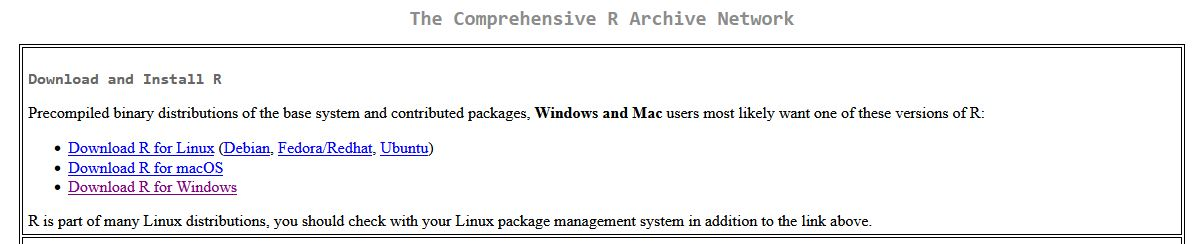
\includegraphics[width=1\linewidth]{./images/telecharger_R_2} 

}

\caption{Choisissez la version adaptée à votre système d'exploitation}\label{fig:dlR2}
\end{figure}

Enfin, installez R à partir du fichier d'installation que vous venez de télécharger.

\subsection{Ouvrez le logiciel R}\label{ouvrez-le-logiciel-r}

Si vous ouvrez le logiciel R, vous aller trouver l'interface graphique de R (\emph{RGui} pour \emph{R Graphical user interface}). Il est possible de faire vos analyses statistiques à partir de cette interface graphique, mais elle est très très austère.

\begin{figure}

{\centering 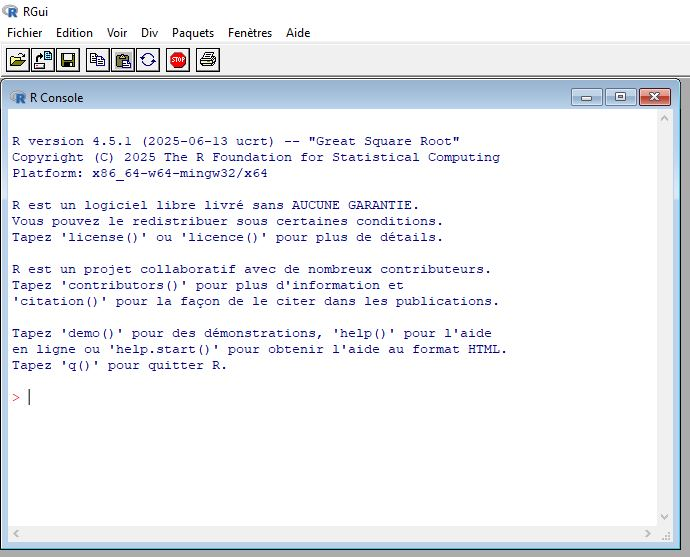
\includegraphics[width=0.5\linewidth]{./images/Rgui} 

}

\caption{L'interface graphique de R (RGui)}\label{fig:RGui}
\end{figure}

Plutôt que d'utiliser cette interface RGui, nous vous recommandons fortement d'utiliser un Environnement de Développement Intégré (IDE), comme RStudio, qui vous facilitera grandement la vie pour utiliser un logiciel statistique qui repose sur de la programmation.

\section{Téléchargez un IDE (RStudio recommandé)}\label{tuxe9luxe9chargez-un-ide-rstudio-recommanduxe9}

RStudio est un environnement qui permet d'utiliser R, mais également d'autres logiciels de programmation comme Python, SQL, Stan, C++, etc. Cet environnement vous facilitera le travail pour :

\begin{itemize}
\tightlist
\item
  éditer vos scripts de programmation,
\item
  accéder à la console,
\item
  visualiser vos environnements de travail avec les fichiers et les objets qu'il contient,
\item
  visualiser vos sorties graphiques et certaines tables d'analyses,
\item
  visualiser vos données,
\item
  visualiser les fichiers d'aide,
\item
  gérer les \emph{packages} permettant de faire des analyses spécifiques,
\item
  et bien d'autres choses encore.
\end{itemize}

Par exemple, le tutoriel que vous êtes en train de lire a été créé à partir du package \href{https://bookdown.org/}{\texttt{bookdown}} avec le logiciels R, au sein de l'IDE RStudio,

Vous pouvez télécharger la dernière version de \href{https://posit.co/download/rstudio-desktop/}{RStudio} sur le site de la compagnie \href{https://posit.co/products/open-source/rstudio/?sid=1}{Posit}. Choisissez la version qui est adaptée à votre système d'exploitation (Windows, macOS ou Linux).

\begin{figure}

{\centering 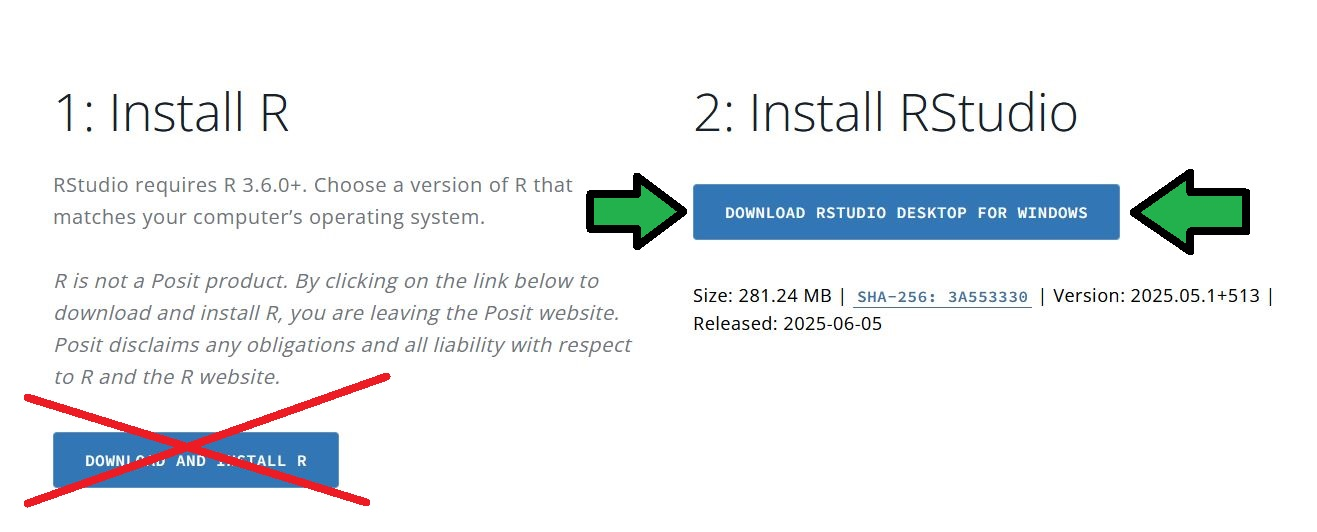
\includegraphics[width=1\linewidth]{./images/telecharger_RStudio_1} 

}

\caption{téléchargez RStudio}\label{fig:dlRStudio-1}
\end{figure}
\begin{figure}

{\centering 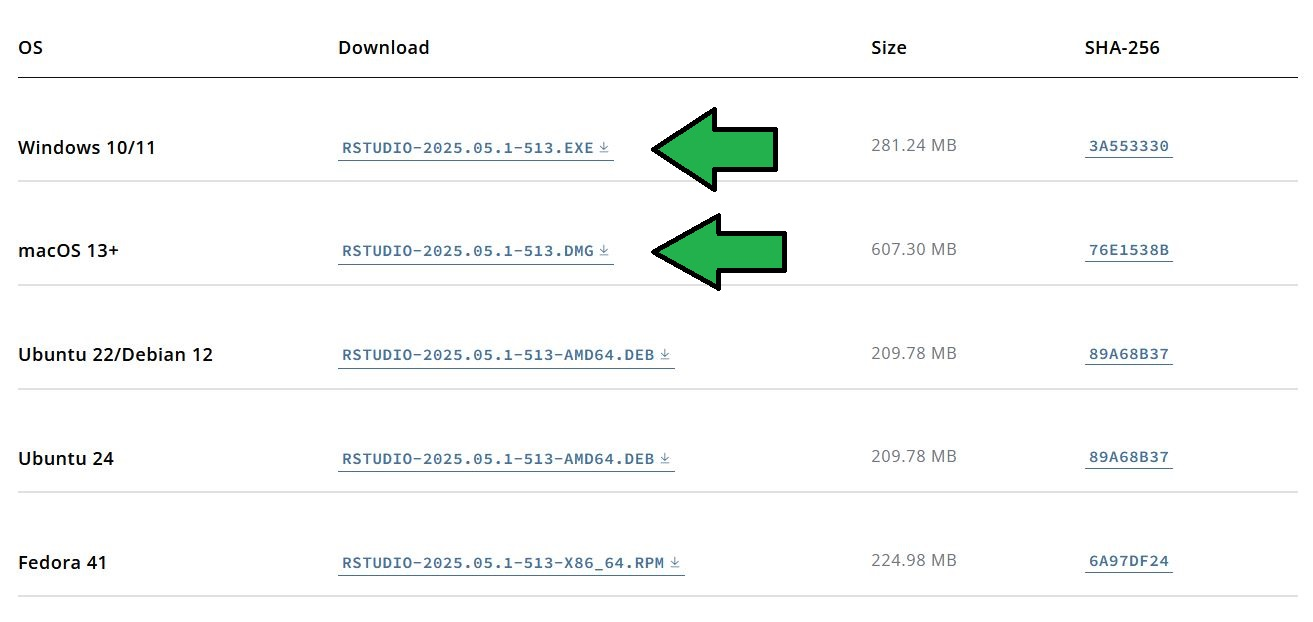
\includegraphics[width=1\linewidth]{./images/telecharger_RStudio_2} 

}

\caption{téléchargez RStudio}\label{fig:dlRStudio-2}
\end{figure}

Puis, installez RStudio à partir du fichier d'installation que vous venez de télécharger.

\subsection{Ouvrez l'IDE RStudio}\label{ouvrez-lide-rstudio}

Ouvrez RStudio, puis commencez par ouvrir un \textbf{script}

\begin{itemize}
\tightlist
\item
  à partir du menu File \textgreater{} New File \textgreater{} R script
\item
  ou bien en utilisant le raccourci Ctrl+Maj+N sur windows
\item
  ou bien en cliquant sur le petit fichier blanc avec un + vert en haut à gauche, puis choisir ``R script''
\end{itemize}

\begin{figure}

{\centering 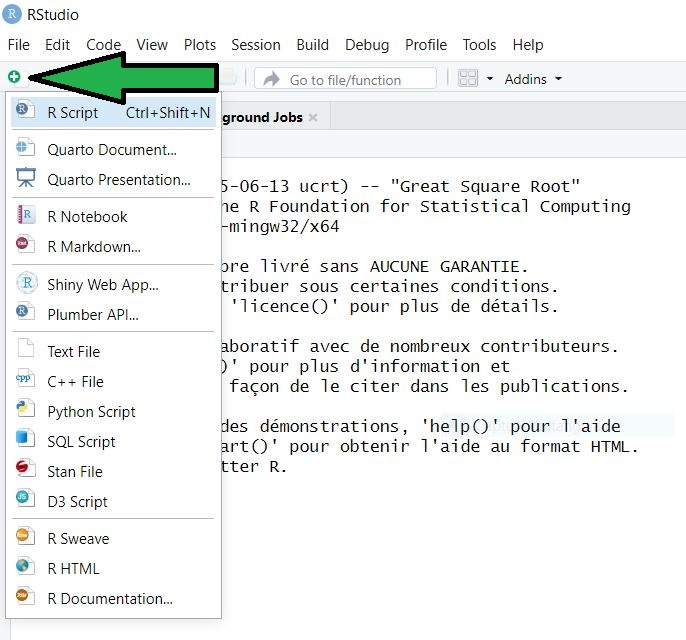
\includegraphics[width=0.5\linewidth]{./images/newscriptR} 

}

\caption{Ouvrir un nouveau script}\label{fig:newscript}
\end{figure}

L'interface de RStudio contient un menu, 4 quadrants et des sous-menus et boutons dans chaque cadrant.

\begin{figure}

{\centering 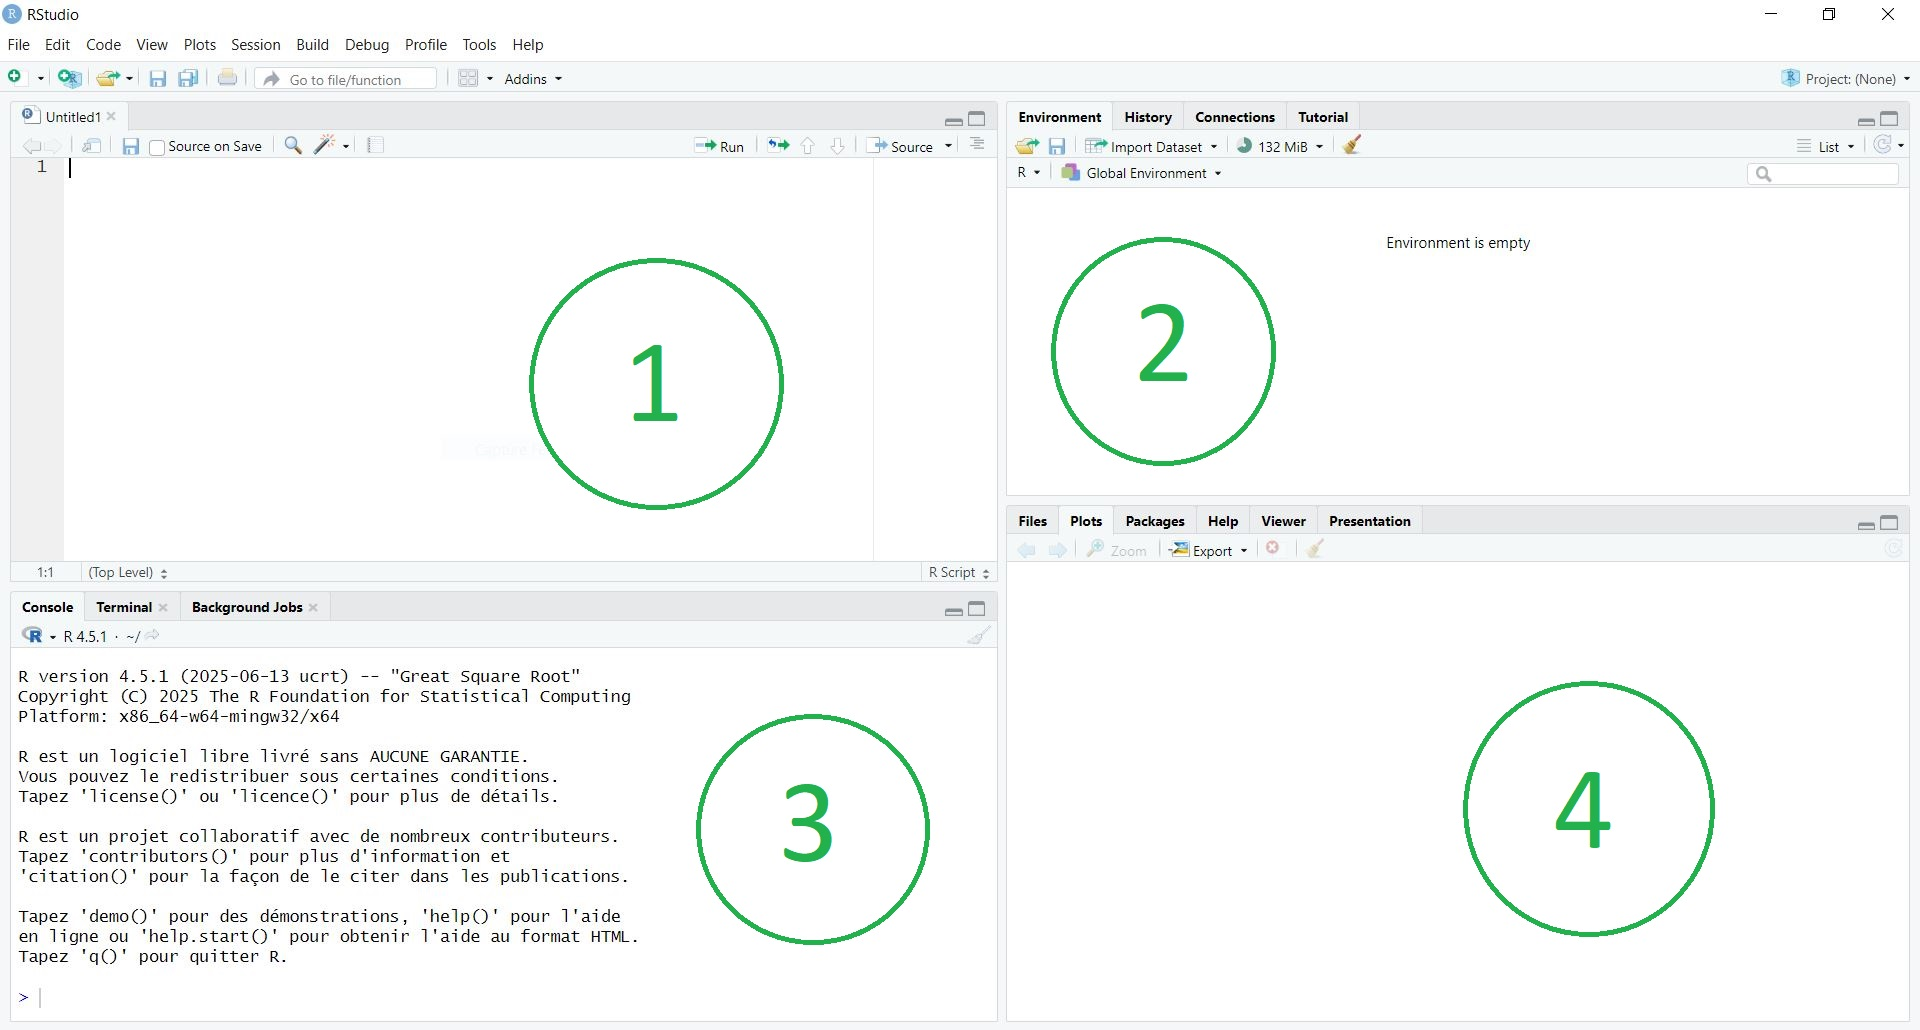
\includegraphics[width=1\linewidth]{./images/cadrants_RStudio} 

}

\caption{Les 4 cadrants de RStudio}\label{fig:RStudcadrants}
\end{figure}

Les menus qui vous seront le plus utiles sont :

\begin{itemize}
\tightlist
\item
  Dans le menu principal,

  \begin{itemize}
  \tightlist
  \item
    le menu \emph{File} vous permettra de créer de nouveaux fichiers, d'ouvrir des fichiers déjà existants, de sauver vos fichiers, d'importer des bases de données, etc.
  \item
    le menu \emph{Tools \textgreater{} Install packages\ldots{}} pour installer de nouveaux packages
  \item
    le menu \emph{Tools \textgreater{} Global Options\ldots{}} vous permet de choisir la version du logiciel R à utiliser (onglet ``R General'') ou bien de changer l'aspect graphique de l'environnement RStudio (onglet ``Appearance'', puis choisissez un ``Editor theme'', avec différentes interfaces claires ou sombres)
  \end{itemize}
\item
  Au sein du \textbf{script} (cadrant 1)

  \begin{itemize}
  \tightlist
  \item
    le bouton ``disquette'' permet de sauvegarder votre script
  \item
    le bouton ``run'' permet de faire tourner votre programme d'analyse (les lignes que vous avez sélectionnées). Par exemple, tapez la commande suivante dans le script, sélectionnez la ligne et cliquez sur le bouton ``run'' (ou avec un raccourci clavier \texttt{ctrl}+\texttt{entrée} sur windows, ou encore \texttt{command}+\texttt{entrée} sur macOS).
  \end{itemize}
\end{itemize}

\begin{Shaded}
\begin{Highlighting}[]
\FunctionTok{print}\NormalTok{(}\StringTok{"Hello Toulouse"}\NormalTok{)}
\end{Highlighting}
\end{Shaded}

et vous devriez voir la commande \texttt{\textgreater{}\ print("Hello\ Toulouse")} puis son résultat \texttt{"Hello\ Toulouse"} dans l'onglet \textbf{console} du cadrant 3.

\begin{itemize}
\tightlist
\item
  Au sein du cadrant 3, l'onglet le plus utile pour pour les débutants est l'onglet \textbf{console}

  \begin{itemize}
  \tightlist
  \item
    la console est la même que la console affichée dans l'interface RGui du logiciel R que l'on a vu au paragraphe 1.2.1.
  \item
    la console commence par afficher la version de R en cours d'utilisation
  \item
    vous pouvez y saisir des commandes et obtenir directement leurs résultats, par exemple si vous tapez dans la console \texttt{4+9}, vous obtiendrez directement le résultat \texttt{13}. \textbf{Attention, les commandes que vous saisissez directement dans la console ne seront pas sauvegardées. Si vous voulez sauvegarder des commandes, il faut utiliser le \emph{script} (cadrant 1)}
  \end{itemize}
\end{itemize}

\begin{Shaded}
\begin{Highlighting}[]
\DecValTok{4}\SpecialCharTok{+}\DecValTok{9}
\end{Highlighting}
\end{Shaded}

\begin{verbatim}
## [1] 13
\end{verbatim}

\begin{itemize}
\tightlist
\item
  Au sein du cadrant 2, l'onglet le plus utile pour les débutants est l'onglet \textbf{Environment}

  \begin{itemize}
  \tightlist
  \item
    cet onglet vous permettra de visualiser les ``objets R'' créés pendant vos analyses.
  \item
    Par exemple si vous saisissez \texttt{v\ \textless{}-\ 1:10} dans la console, vous allez voir apparaître l'objet \texttt{v} dans l'environnement de travail (il s'agit d'un vecteur de 1 à 10, nommé ``v'').
  \end{itemize}
\item
  Au sein du cadrant 4, les onglets les plus utiles pour les débutants sont :

  \begin{itemize}
  \tightlist
  \item
    l'onglet ``File'' qui contient les dossiers et fichiers au sein d'un dossier de travail (voir le chapitre 3 pour créer et organiser un dossier de travail associé à un ``projet R'')
  \item
    l'onglet ``Plots'' où vous retrouverez vos sorties graphiques. Au sein de cet onglet, vous trouverez un menu pour exporter vos graphiques selon différents formats. Des boutons permettent également de zoomer et d'effacer les graphiques. Par exemple, si vous saisissez \texttt{hist(rnorm(10000))} dans la console, un histogramme d'une distribution normale centrée réduite va apparaître. Vous pouvez effacer la figure en cliquant sur le bouton avec la croix rouge (efface la figure actuelle) ou le balet (efface l'ensemble des figures).
  \item
    l'onglet ``Packages'' où vous pourrez activer, désactiver ou mettre à jour les packages qui ont été téléchargés.
  \item
    l'onglet ``Help'' où vous trouverez de l'aide. Par exemple si vous saisissez \texttt{help(mean)} dans la console, l'aide de la commande \texttt{mean} va s'afficher. Vous pouvez également utiliser le champ de recherche de fonctions dans le menu ``Help''.
  \end{itemize}
\end{itemize}

\section{Trouver de l'aide sur R}\label{trouver-de-laide-sur-r}

De nombreuses ressources sont disponibles pour vous aider à utiliser R :

\begin{itemize}
\item
  Les pages d'aide en ligne de R, qui apparaîssent directement dans RStudio. Vous pouvez obtenir de l'aide sur des fonctions et des packages :

  \begin{itemize}
  \tightlist
  \item
    en appliquant une recherche par mot clé dans le champ de recherche de l'onglet ``help''
  \item
    en utilisant directement dans la console la fonction \texttt{help.search()} ou \texttt{??} associée à un mot clé (par exemple \texttt{help.search(student)} ou \texttt{??student}), ou la fonction \texttt{help()} associée à une fonction (par exemple \texttt{help(t.test)} ou \texttt{?t.test})
  \item
    quand vous rencontrerez une nouvelle fonction (dans ce cours ou bien dans votre pratique), nous vous conseillons d'aller systématiquement regarder l'aide de cette fonction pour bien comprendre comment l'utiliser.
  \item
    Ces pages d'aide suivent la structure suivante :

    \begin{itemize}
    \tightlist
    \item
      une partie ``Description'' qui décrit en quelques phrases ce que fait la fonction
    \item
      une partie ``Usage'' qui décrit la syntaxe de la fonction avec ses arguments
    \item
      une partie ``Argument'' qui précise comment renseigner les arguments de la fonction
    \item
      une partie ``Detail'' qui décrit en détail comment utiliser la fonction et ses arguments
    \item
      une partie ``Value'' qui décrit les sorties (les résultats) de la fonction, avec les éventuels sous-objets de la sortie
    \item
      une partie ``Exemples'' qui indique quelques exemple que vous pouvez directement lancer en cliquant sur ``Run examples''
    \end{itemize}
  \end{itemize}
\item
  Des fiches ``mémoires'' \emph{cheat sheets} qui résument les principales fonctions :

  \begin{itemize}
  \tightlist
  \item
    pour les \href{https://rstudio.github.io/cheatsheets/base-r.pdf}{commandes R bases}
  \item
    des \href{https://rstudio.github.io/cheatsheets/R-best-practice.pdf}{bonnes pratiques sur R}
  \item
    méthodes de visualisation avec le package \href{https://posit.co/wp-content/uploads/2022/10/data-visualization-1.pdf}{ggplot2}
  \item
    méthodes de manipulation de données avec le package \href{https://rstudio.github.io/cheatsheets/html/tidyr.html}{tidyr}
  \item
    méthodes de transformation de données avec le package \href{https://rstudio.github.io/cheatsheets/html/data-transformation.html}{dplyr}
  \item
    l'utilisation du package \href{https://rstudio.github.io/cheatsheets/datatable.pdf}{data.table}
  \item
    l'utilisation du package \href{https://rstudio.github.io/cheatsheets/html/strings.html}{stringr} pour manipuler les chaînes de caractères, avec la \href{https://rstudio.github.io/cheatsheets/strings.pdf}{fiche stringr}
  \item
    la manipulation de dates \href{https://rstudio.github.io/cheatsheets/html/lubridate.html}{Dates and times with lubridate} et la \href{https://rstudio.github.io/cheatsheets/lubridate.pdf}{fiche lubridate}
  \end{itemize}
\item
  De nombreux livres et tutoriels disponibles gratuitement en ligne :

  \begin{itemize}
  \tightlist
  \item
    Le \href{https://larmarange.github.io/guide-R/}{guide R} de Joseph Larmarange, est un guide très complet et didactique, en français
  \item
    L'\href{https://epirhandbook.com/en/index.html}{Epidemiologist R Handbook} est un tutoriel en anglais pour l'utilisation de R par des épidémiologistes
  \item
    Software carpentry met à disposition des guides introductifs bien réalisés en anglais, par exemple \href{https://swcarpentry.github.io/r-novice-gapminder/}{R for Reproducible Scientific Analysis} ou encore \href{https://swcarpentry.github.io/r-novice-inflammation/}{Programming with R}
  \item
    le livre \href{https://r4ds.hadley.nz/}{R for Data Science} propose une introduction très complète pour l'analyse de données descriptive principalement basée sur la suite de packages du \href{https://www.tidyverse.org/}{Tidyverse}
  \item
    le package R \href{https://swirlstats.com/}{swirl} propose une formation interactive directement dans la console de RStudio, téléchargez le package (\texttt{install.packages("swirl")}), chargez le package (\texttt{library("swirl")}) et laissez vous guider après avoir saisi \texttt{swirl()} dans la console.
  \item
    \href{https://education.rstudio.com/learn/beginner/}{RStudio Education} liste plusieurs ressources intéressantes pour les débutants
  \item
    Le site CRAN a des manuels assez complets, par exemple la page \href{https://cran.r-project.org/doc/manuals/R-lang.html}{R Language Definition} est une introduction assez complète au langage de programmation R. La page \href{https://cran.r-project.org/web/views/}{CRAN Task Views} liste les packages qui sont disponibles par thématique ou type d'anlayse.
  \end{itemize}
\item
  Rechercher à l'aide d'un moteur de recherche (google, DuckDuckGo, Bing, etc). Ces recherches vous amèneront régulièrement vers des forums de discussion comme \href{https://stackoverflow.com/questions/tagged/R}{stackoverflow} ou \href{https://stats.stackexchange.com/questions/tagged/r}{stackExchange}. Si vous rencontrez une erreur ou une difficulté, il y a toutes les chances que d'autres personnes aient déjà rencontré ces erreurs et difficultés avant vous, et que des solutions détaillées soient proposées dans ces forums.
\item
  Les chatbots de type GPT, Copilot ou Gemini : dans le cadre de votre formation au logiciel R, nous vous déconseillons l'utilisation de ces outils basés sur des LLM. Ces outils posent de nombreux problèmes en termes de transparence, de respect de droit d'auteur, d'impact environnemental, de déqualification (délegation de compétences pour rechercher de l'information, perte d'esprit critique), de dépendance aux Gafams, de dégradation des systèmes d'information, etc. Par ailleurs, bien qu'ils peuvent apporter des solutions fonctionnelles, il est bien plus utile d'avoir une bonne compréhension des bases de programmations sur R avant d'utiliser de tels outils : sans une bonne compréhension de la logique de programmation et des principales fonctions de R, vous aurez des difficultés à évaluer la fiabilité des solutions proposées, à vous débloquez en cas de problèmes, ou encore à adapter vos prompts pour obtenir de meilleures réponses. Les ressources décrites précédemment devraient vous permettre d'apporter efficacement des réponses à vos questions.
\end{itemize}

\section{Conventions d'écriture}\label{conventions-duxe9criture}

Certaines conventions ont été proposées pour faciliter l'écriture et la lecture du code de programmation dans R. Elles ne sont pas obligatoires, mais nous vous encourrageons à les suivre.

Par exemple, le \href{https://style.tidyverse.org/}{\emph{Tidyverse style guide}} :

\begin{itemize}
\tightlist
\item
  nommer les variables et les fonctions en lettres minuscules, à l'aide de mots et de chiffres séparés par \texttt{\_} (\emph{underscore}). Par exemple \texttt{csp\_1}. Cette convention fait référence au style \href{https://en.wikipedia.org/wiki/Snake_case}{``snake case''}
\item
  ajouter un espace après une virgule, par exemple \texttt{x{[}2,\ 5{]}}
\item
  ajouter des espaces avant et après les opérateurs arithmétiques, par exemple \texttt{x\ \textless{}-\ (1\ +\ 2)\ /\ 5}, à quelques exceptions près (pas d'espace avant ou après le signe ``puissance'' \texttt{\^{}}) \texttt{y\ \textless{}-\ x\^{}2\ +\ 3}
\end{itemize}

\chapter{Les objets dans R}\label{les-objets-dans-r}

La programmation R repose sur des \emph{objets}, qui apparaîtront dans la fenêtre \emph{Environment} de RStudio.

Les objets les plus élémentaires dans R sont des \textbf{vecteurs}. Un vecteur contient une série de valeurs (des nombres, des chaînes de caractères, ou des données plus complexes). Il y a deux types de vecteurs :

\begin{itemize}
\tightlist
\item
  les \textbf{vecteurs atomiques} (les valeurs d'un vecteur atomique doivent toujours être du même type),
\item
  les \textbf{listes} (les valeurs d'une liste peuvent être de différents types).
\end{itemize}

\section{Manipuler les objets dans l'environnement}\label{manipuler-les-objets-dans-lenvironnement}

Voici quelques commandes de gestion des objets dans votre environnement :

\begin{itemize}
\tightlist
\item
  dans la console, commencez par créer les objets suivants. Pour \textbf{assigner une ou plusieurs valeurs à un objet}, on utilise une flèche dirigée vers la gauche \texttt{\textless{}-}. Vous verrez apparaître ces objets dans la fenêtre \emph{Environment}.
\end{itemize}

\begin{Shaded}
\begin{Highlighting}[]
\DocumentationTok{\#\# note : le signe dièze (\#) permet d\textquotesingle{}ajouter des commentaires dans le code  }
\DocumentationTok{\#\# {-} le 1er objet est un vecteur de 10 nombres entiers de 1 à 10}
\DocumentationTok{\#\# {-} le 2ème objet est un vecteur de 3 lettres A, B et C}
\DocumentationTok{\#\# {-} le 3ème objet est un vecteur de 2 réels, calculés par 2 opérations}
\DocumentationTok{\#\# {-} le 4ème objet est une fonction qui ajoute 2 aux éléments du vecteur x}
\DocumentationTok{\#\# {-} le 5ème objet est un scalaire égal à 42}
\NormalTok{objet\_1 }\OtherTok{\textless{}{-}} \FunctionTok{c}\NormalTok{(}\DecValTok{1}\SpecialCharTok{:}\DecValTok{10}\NormalTok{) }
\NormalTok{objet\_2 }\OtherTok{\textless{}{-}} \FunctionTok{c}\NormalTok{(}\StringTok{"A"}\NormalTok{, }\StringTok{"B"}\NormalTok{, }\StringTok{"C"}\NormalTok{) }
\NormalTok{objet\_3 }\OtherTok{\textless{}{-}} \FunctionTok{c}\NormalTok{(}\DecValTok{10} \SpecialCharTok{/} \DecValTok{3}\NormalTok{, }\DecValTok{4} \SpecialCharTok{*} \DecValTok{5}\NormalTok{) }
\NormalTok{objet\_4 }\OtherTok{\textless{}{-}} \ControlFlowTok{function}\NormalTok{(x) \{x }\SpecialCharTok{+} \DecValTok{2}\NormalTok{\} }
\NormalTok{objet\_5 }\OtherTok{\textless{}{-}} \DecValTok{42} 
\end{Highlighting}
\end{Shaded}

\begin{itemize}
\tightlist
\item
  la commande \texttt{ls()} permet de \textbf{lister} les objets dans l'environnement.
\item
  la commande \texttt{rm()} permet de \textbf{supprimer} (\emph{remove}) un ou plusieurs objets de l'environnement.
\end{itemize}

\begin{Shaded}
\begin{Highlighting}[]
\FunctionTok{ls}\NormalTok{()}
\end{Highlighting}
\end{Shaded}

\begin{verbatim}
## [1] "objet_1" "objet_2" "objet_3" "objet_4" "objet_5"
\end{verbatim}

\begin{Shaded}
\begin{Highlighting}[]
\FunctionTok{rm}\NormalTok{(objet\_2, objet\_5)}
\FunctionTok{rm}\NormalTok{(}\AttributeTok{list =} \FunctionTok{ls}\NormalTok{()) }\CommentTok{\# pour supprimer tous les objets présents dans l\textquotesingle{}environnement}
\end{Highlighting}
\end{Shaded}

Conseils pour nommer un objet dans R :

\begin{itemize}
\tightlist
\item
  Utiliser des noms courts, mais lisibles, faciles à comprendre
\item
  Les noms doivent commencer par une lettre (pas par un nombre) et ne peuvent pas contenir d'espace. A noter qu'ils peuvent contenir des points, comme par exemple \texttt{nom.variable}.
\item
  Evitez d'utiliser des noms de variables et de fonctions déjà existants dans R (par exemple \texttt{mean} qui risque de porter à confusion avec la fonction \texttt{mean()} : il vaut mieux utiliser \texttt{mean\_variable})
\item
  Ecrire en minuscule avec underscore pour séparer les mots (par exemple \texttt{date\_naissance})
\end{itemize}

\section{Principaux types de données}\label{principaux-types-de-donnuxe9es}

Les données peuvent être de différents types. Les 4 principaux types sont :

\begin{itemize}
\tightlist
\item
  les \textbf{nombres réels} (\texttt{?double}), par exemple \texttt{12.43}.
\item
  les \textbf{nombres entiers} (\texttt{?integer}). Les nombres entiers sont saisis en ajoutant \texttt{L} à droite du nombre, par exemple \texttt{5L}.
\item
  les \textbf{chaînes de caractères textuels} (\texttt{?character}), définis avec des guillemets simples ou doubles , par exemple \texttt{\textquotesingle{}bonjour\textquotesingle{}} ou \texttt{"au\ revoir"}
\item
  les \textbf{valeurs logiques} (\texttt{?logical}), avec deux valeurs possibles :

  \begin{itemize}
  \tightlist
  \item
    valeur booléenne \emph{vraie}, notée \texttt{TRUE} ou bien \texttt{T}
  \item
    valeur booléenne \emph{fausse}, notée \texttt{FALSE} ou bien \texttt{F}
  \end{itemize}
\end{itemize}

On peut également trouver des types de données un peu plus sophistiquées, construites à partir des principaux types :

\begin{itemize}
\tightlist
\item
  des \textbf{variables qualitatives} qui peuvent être \textbf{nominales} (\texttt{?factor}) ou \textbf{ordinales} (\texttt{?ordered}). Ces variables sont construites sur des nombres entiers.
\item
  des \textbf{dates} (\texttt{?Date}), qui sont construites sur des nombres réels.
\item
  des \textbf{dates-heure} (\texttt{?POSIXct}), qui sont construites sur des nombres réels.
\item
  des \textbf{durées} (\texttt{?difftime}), construites sur des nombres réels.
\end{itemize}

On a également un vecteur particulier qui est le \textbf{vecteur nul} et se note \texttt{NULL}. Le vecteur nul a une longueur de 0 et ne peut avoir aucun attribut (les notions de longueur et d'attribut d'un vecteur seront vues plus bas).

\subsection{Données manquantes}\label{donnuxe9es-manquantes}

Quel que soit le type de données, les données manquantes se notent \texttt{NA} (not applicable).

Attention à ne pas confondre le vecteur nul \texttt{NULL} et les données manquantes \texttt{NA}.

\subsection{\texorpdfstring{Décrire le type de l'objet \(\spadesuit\)}{Décrire le type de l'objet \textbackslash spadesuit}}\label{duxe9crire-le-type-de-lobjet-spadesuit}

Les paragraphes avec un \(\spadesuit\) présentent des notions plus avancées, si vous êtes en phase d'apprentissage, vous pouvez aller directement au paragraphe suivant.

On peut décrire quel est le type de l'objet avec les fonctions \texttt{typeof} (le type le plus élémentaire), \texttt{mode} et \texttt{storage.mode} (mode de l'objet et mode de stockage de l'objet selon un regroupement un peu plus large).

Par exemple, les nombres réels (\texttt{double}) et les nombres entiers (\texttt{integer}) sont du mode \texttt{numeric}.

\begin{Shaded}
\begin{Highlighting}[]
\DocumentationTok{\#\# les valeurs réelles (\textquotesingle{}double\textquotesingle{}) et les entiers (\textquotesingle{}integer\textquotesingle{}) sont de mode \textquotesingle{}numeric\textquotesingle{}}
\FunctionTok{typeof}\NormalTok{(}\FloatTok{2.53}\NormalTok{) }\CommentTok{\# un réel}
\FunctionTok{typeof}\NormalTok{(}\DecValTok{5}\DataTypeTok{L}\NormalTok{) }\CommentTok{\# et un entier}
\FunctionTok{mode}\NormalTok{(}\FloatTok{2.53}\NormalTok{) }\CommentTok{\# sont de mode \textquotesingle{}numeric\textquotesingle{}}
\FunctionTok{mode}\NormalTok{(}\DecValTok{5}\DataTypeTok{L}\NormalTok{)}
\FunctionTok{storage.mode}\NormalTok{(}\FloatTok{2.53}\NormalTok{)}
\FunctionTok{storage.mode}\NormalTok{(}\DecValTok{5}\DataTypeTok{L}\NormalTok{)}

\DocumentationTok{\#\# les chaînes de caractères sont de type et de mode \textquotesingle{}character\textquotesingle{}}
\FunctionTok{typeof}\NormalTok{(}\FunctionTok{c}\NormalTok{(}\StringTok{"hello"}\NormalTok{, }\StringTok{"Toulouse"}\NormalTok{))}
\FunctionTok{mode}\NormalTok{(}\FunctionTok{c}\NormalTok{(}\StringTok{"hello"}\NormalTok{, }\StringTok{"Toulouse"}\NormalTok{))}

\DocumentationTok{\#\# les valeurs logiques sont de type \textquotesingle{}logical\textquotesingle{}}
\FunctionTok{typeof}\NormalTok{(}\FunctionTok{c}\NormalTok{(}\ConstantTok{TRUE}\NormalTok{, }\ConstantTok{FALSE}\NormalTok{, }\ConstantTok{FALSE}\NormalTok{))}
\FunctionTok{mode}\NormalTok{(}\FunctionTok{c}\NormalTok{(}\ConstantTok{TRUE}\NormalTok{, }\ConstantTok{FALSE}\NormalTok{, }\ConstantTok{FALSE}\NormalTok{))}
\end{Highlighting}
\end{Shaded}

\begin{longtable}[]{@{}
  >{\centering\arraybackslash}p{(\linewidth - 6\tabcolsep) * \real{0.3205}}
  >{\centering\arraybackslash}p{(\linewidth - 6\tabcolsep) * \real{0.2308}}
  >{\centering\arraybackslash}p{(\linewidth - 6\tabcolsep) * \real{0.2051}}
  >{\centering\arraybackslash}p{(\linewidth - 6\tabcolsep) * \real{0.2436}}@{}}
\toprule\noalign{}
\begin{minipage}[b]{\linewidth}\centering
\texttt{x}
\end{minipage} & \begin{minipage}[b]{\linewidth}\centering
\texttt{typeof(x)}
\end{minipage} & \begin{minipage}[b]{\linewidth}\centering
\texttt{mode(x)}
\end{minipage} & \begin{minipage}[b]{\linewidth}\centering
\texttt{storage.mode(x)}
\end{minipage} \\
\midrule\noalign{}
\endhead
\bottomrule\noalign{}
\endlastfoot
\texttt{2.53} & \texttt{"double"} & \texttt{"numeric"} & \texttt{"double"} \\
\texttt{5L} & \texttt{"integer"} & \texttt{"numeric"} & \texttt{"integer"} \\
\texttt{"bonjour"} & \texttt{"character"} & \texttt{"character"} & \texttt{"character"} \\
\texttt{TRUE} & \texttt{"logical"} & \texttt{"logical"} & \texttt{"logical"} \\
\texttt{as.Date("2025-07-01")} & \texttt{"double"} & \texttt{"numeric"} & \texttt{"double"} \\
\end{longtable}

Les fonctions \texttt{as.double}, \texttt{as.integer}, \texttt{as.character}, \texttt{as.logical} permettent de forcer par coercition le type d'un objet \emph{en tant que} réel, entier, chaîne de caractères, logique.

\begin{Shaded}
\begin{Highlighting}[]
\FunctionTok{as.double}\NormalTok{(}\DecValTok{5}\DataTypeTok{L}\NormalTok{) }\CommentTok{\# définit un nombre entier en tant que nombre réel}
\FunctionTok{as.integer}\NormalTok{(}\FloatTok{4.95}\NormalTok{) }\CommentTok{\# définit un réel en tant qu\textquotesingle{}entier, seul l\textquotesingle{}entier est conservé}
\FunctionTok{as.character}\NormalTok{(}\FloatTok{4.95}\NormalTok{) }\CommentTok{\# définit un nombre en tant que chaîne de caractères}

\DocumentationTok{\#\# définir une valeur logique TRUE et FALSE en tant que valeur numérique }
\DocumentationTok{\#\# ou en tant qu\textquotesingle{}entier donne les valeurs 1 et 0, respectivement}
\FunctionTok{as.numeric}\NormalTok{(}\ConstantTok{TRUE}\NormalTok{) }
\FunctionTok{as.numeric}\NormalTok{(}\ConstantTok{FALSE}\NormalTok{) }

\DocumentationTok{\#\# définir le nombre 0 en tant que valeur logique donne la valeur FALSE}
\FunctionTok{as.logical}\NormalTok{(}\DecValTok{0}\NormalTok{)}

\DocumentationTok{\#\# définir tout nombre différent de 0 en tant que valeur logique }
\DocumentationTok{\#\# donne la valeur TRUE}
\FunctionTok{as.logical}\NormalTok{(}\SpecialCharTok{{-}}\DecValTok{14}\NormalTok{)}
\FunctionTok{as.logical}\NormalTok{(}\DecValTok{1}\NormalTok{)}
\FunctionTok{as.logical}\NormalTok{(}\FloatTok{4.95}\NormalTok{)}
\end{Highlighting}
\end{Shaded}

Les fonctions \texttt{is.double}, \texttt{is.integer}, \texttt{is.character}, \texttt{is.logical} permettent d'évaluer si un objet est de type réel, entier, textuel, logique.

\begin{Shaded}
\begin{Highlighting}[]
\FunctionTok{is.double}\NormalTok{(}\DecValTok{5}\DataTypeTok{L}\NormalTok{) }\CommentTok{\# FALSE, un nombre de type "entier" n\textquotesingle{}est pas de type "réel"}
              \CommentTok{\# attention, en math, les nombres entiers font partie des réels !}
\FunctionTok{is.integer}\NormalTok{(}\FloatTok{4.95}\NormalTok{) }\CommentTok{\# FALSE, un nombre de type "réel" n\textquotesingle{}est pas de type "entier"}
\FunctionTok{is.numeric}\NormalTok{(}\StringTok{"bonjour"}\NormalTok{) }\CommentTok{\# FALSE "bonjour" est une chaîne de caractères}
\FunctionTok{is.character}\NormalTok{(}\StringTok{"bonjour"}\NormalTok{) }\CommentTok{\# TRUE, "bonjour" est bien une chaîne de caractères}
\FunctionTok{is.character}\NormalTok{(}\FloatTok{4.95}\NormalTok{) }\CommentTok{\# FALSE, 4.95 est un objet numérique}
\FunctionTok{is.logical}\NormalTok{(}\DecValTok{1}\NormalTok{) }\CommentTok{\# FALSE, 1 est un objet numérique}
\FunctionTok{is.logical}\NormalTok{(}\FunctionTok{as.logical}\NormalTok{(}\DecValTok{1}\NormalTok{)) }\CommentTok{\# TRUE, as.logical(1) = TRUE, qui est un objet logique}
\FunctionTok{is.logical}\NormalTok{(}\ConstantTok{TRUE}\NormalTok{) }\CommentTok{\# TRUE est bien un objet logique}
\end{Highlighting}
\end{Shaded}

\section{Principales structures de données}\label{principales-structures-de-donnuxe9es}

Les principales structures de données que nous allons détailler dans la suite de ce chapitre sont :

\begin{itemize}
\tightlist
\item
  les \textbf{vecteurs atomiques} (\texttt{?c()}), qui doivent toujours comporter des valeurs du même type. Les vecteurs qui ne comportent qu'une seule valeur sont appelés des ``scalaires'' ;
\item
  les \textbf{listes} (\texttt{?list}), qui sont également des vecteurs, mais peuvent comporter des valeurs de types différents ;
\item
  les \textbf{matrices} (\texttt{?matrix}, \texttt{?array}), qui sont des vecteurs atomiques réarrangés sous forme de tables à 2 dimensions ou plus ;
\item
  les \textbf{bases de données} (\texttt{?data.frames}). Les bases de données sont des listes de vecteurs atomiques de même longueur. Il existe d'autres formats de base de données qui seront présentés plus tard (avec les packages \texttt{tidyverse} et \texttt{data.table}).
\end{itemize}

\section{Objet à une seule valeur (scalaire ou texte)}\label{objet-uxe0-une-seule-valeur-scalaire-ou-texte}

\subsection{Scalaires}\label{scalaires}

Assignez les valeurs 4 et 5 à deux objets

\begin{Shaded}
\begin{Highlighting}[]
\NormalTok{x\_1 }\OtherTok{\textless{}{-}} \DecValTok{4}
\NormalTok{x\_2 }\OtherTok{\textless{}{-}} \DecValTok{5}
\end{Highlighting}
\end{Shaded}

\subsection{Opérations mathématiques sur les scalaires}\label{opuxe9rations-mathuxe9matiques-sur-les-scalaires}

\subsubsection{Calculatrice}\label{calculatrice}

On peut utiliser les opérations classiques, comme sur une calculatrice :

\begin{itemize}
\tightlist
\item
  \texttt{+} pour \textbf{additionner}
\item
  \texttt{-} pour \textbf{soustraire}
\item
  \texttt{*} pour \textbf{multiplier}
\item
  \texttt{/} pour \textbf{diviser}
\item
  \texttt{\^{}} pour mettre à la \textbf{puissance}
\item
  \texttt{e} pour la \textbf{notation scientifique}
\end{itemize}

\begin{Shaded}
\begin{Highlighting}[]
\NormalTok{x\_1 }\SpecialCharTok{+}\NormalTok{ x\_2 }\CommentTok{\# 4 + 5 = 9}
\DecValTok{10} \SpecialCharTok{{-}}\NormalTok{ x\_1 }\CommentTok{\# 10 {-} 4 = 6}
\NormalTok{x\_1 }\SpecialCharTok{*}\NormalTok{ x\_2 }\CommentTok{\#  4 * 5 = 20}
\DecValTok{20} \SpecialCharTok{/}\NormalTok{ x\_2 }\CommentTok{\# 20 / 5 = 4}
\NormalTok{x\_1}\SpecialCharTok{\^{}}\DecValTok{2} \CommentTok{\#  4\^{}2 = 16}
\DecValTok{10}\SpecialCharTok{\^{}{-}}\DecValTok{1} \CommentTok{\# 1/10 = 0.1}
\DecValTok{25}\SpecialCharTok{\^{}}\NormalTok{(}\FloatTok{0.5}\NormalTok{) }\CommentTok{\# racine carrée de 25 (puissance 1/2)}

\DocumentationTok{\#\# notation scientifique pour les grands et petits nombres}
\DecValTok{1}\SpecialCharTok{/}\DecValTok{1000000} \CommentTok{\# 1 pour 1 million = 1e{-}6}
\DecValTok{1}\SpecialCharTok{/}\FloatTok{1e6}
\FloatTok{1e6} \SpecialCharTok{*} \DecValTok{1000} \CommentTok{\# 1 million * 1000 = 1 milliard}
\end{Highlighting}
\end{Shaded}

\subsubsection{Fonctions mathématiques}\label{fonctions-mathuxe9matiques}

Plusieurs fonctions mathématiques de bases sont implémentées nativement dans R :

\begin{itemize}
\tightlist
\item
  \texttt{log(x)} ou \texttt{log(x,\ base\ =\ exp(1))} pour le \textbf{logarithme} népérien,
\item
  \texttt{log10(x)} pour le logarithme base 10, \texttt{log2(x)} pour le logarithme base 2,
\item
  \texttt{log(x,\ base\ =\ b)} pour le logarithme base \texttt{b},
\item
  \texttt{exp(x)} pour l'\textbf{exponentielle} de \texttt{x}
\item
  \texttt{sqrt(x)} pour la \textbf{racine carrée} de \texttt{x}
\item
  \texttt{abs(x)} pour la \textbf{valeur absolue} de \texttt{x}
\item
  les \textbf{fonctions trigonométriques} sont implémentées, avec \texttt{cos(x)}, \texttt{sin(x)}, \texttt{tan(x)} (cf.~\texttt{?Trig})
\item
  la \textbf{constante \(\pi\)} est implémentée avec \texttt{pi} (cf.~\texttt{?Constants})
\end{itemize}

Si vous appliquer une fonction à une valeur qui ne fait pas partie du domaine de définition de la fonction, le résultat sera une valeur manquante notée \texttt{NaN} (\emph{not a number}). Un message d'avertissement va apparaître si vous appliquez une fonction en dehors de son domaine de définition.

Les notions de + l'infini et - l'infini sont notées \texttt{Inf} et \texttt{-Inf}.

\begin{Shaded}
\begin{Highlighting}[]
\DocumentationTok{\#\# logarithmes et exponentielles}
\FunctionTok{log}\NormalTok{(}\DecValTok{1}\NormalTok{)}
\FunctionTok{log10}\NormalTok{(}\DecValTok{100}\NormalTok{)}
\FunctionTok{log}\NormalTok{(}\DecValTok{100}\NormalTok{, }\AttributeTok{base =} \DecValTok{10}\NormalTok{)}
\FunctionTok{exp}\NormalTok{(}\DecValTok{1}\NormalTok{)}

\DocumentationTok{\#\# racine carrée}
\FunctionTok{sqrt}\NormalTok{(x\_2}\SpecialCharTok{\^{}}\DecValTok{2}\NormalTok{)}

\DocumentationTok{\#\# valeur absolue}
\FunctionTok{abs}\NormalTok{(}\DecValTok{10}\NormalTok{)}
\FunctionTok{abs}\NormalTok{(}\SpecialCharTok{{-}}\DecValTok{10}\NormalTok{)}

\DocumentationTok{\#\# fonctions trigonométriques}
\FunctionTok{cos}\NormalTok{(}\DecValTok{1}\NormalTok{)}
\FunctionTok{sin}\NormalTok{(}\DecValTok{1}\NormalTok{)}
\FunctionTok{tan}\NormalTok{(}\DecValTok{1}\NormalTok{)}
\NormalTok{pi}
\DecValTok{2} \SpecialCharTok{*}\NormalTok{ pi }\SpecialCharTok{*} \DecValTok{10} \CommentTok{\# circonférence d\textquotesingle{}un cercle de rayon 10}

\DocumentationTok{\#\# si on utilise une valeur en dehors du domaine d\textquotesingle{}application de la fonction}
\FunctionTok{log}\NormalTok{(}\SpecialCharTok{{-}}\DecValTok{1}\NormalTok{) }\CommentTok{\# NaN, car {-}1 est en dehors du domaine de définition de la fonction log}
\FunctionTok{sqrt}\NormalTok{(}\SpecialCharTok{{-}}\DecValTok{2}\NormalTok{) }\CommentTok{\# {-}2 est en dehors du domaine de définition de la fonction racine carrée}

\DocumentationTok{\#\# notions de + ou {-} l\textquotesingle{}infini}
\DecValTok{1} \SpecialCharTok{/} \DecValTok{0} \CommentTok{\# [1] Inf}
\SpecialCharTok{{-}}\DecValTok{1} \SpecialCharTok{/} \DecValTok{0} \CommentTok{\# [1] {-}Inf}
\end{Highlighting}
\end{Shaded}

\subsubsection{\texorpdfstring{Fonctions d'arrondi \(\spadesuit\)}{Fonctions d'arrondi \textbackslash spadesuit}}\label{fonctions-darrondi-spadesuit}

Plusieurs fonctions sont disponibles dans R pour arrondir une valeur (cf.~\texttt{?Round}) :

\begin{itemize}
\tightlist
\item
  la fonction \texttt{round()} est utile pour arrondir les décimales. Il faut préciser en argument le nombre de chiffres après la virgule. \textbf{Attention} : si le nombre se termine par un 5, l'arrondi se fait vers le chiffre pair le plus proche : 4,45 s'arrondit à 4,4 (la valeur arrondie inférieure) et 4,75 s'arrondit à 4,8 (la valeur arrondie supérieure)
\item
  la fonction \texttt{signif()} arrondit aux chiffres les plus significatifs (les plus grands)
\item
  la fonction \texttt{floor()} arrondit la valeur à l'entier inférieur
\item
  la fonction \texttt{ceiling()} arrondit la valeur à l'entier supérieur
\item
  la fonction \texttt{trunc()} ne garde que les entiers, sans arrondir
\end{itemize}

\begin{Shaded}
\begin{Highlighting}[]
\DocumentationTok{\#\# fonction round()}
\CommentTok{\# l\textquotesingle{}argument digits permet de définir le nombre de chiffres après la virgule}
\CommentTok{\# exemple si vous voulez arrondir à 2 chiffres après la virgule}
\FunctionTok{round}\NormalTok{(}\FloatTok{0.09400}\NormalTok{, }\AttributeTok{digits =} \DecValTok{2}\NormalTok{) }\CommentTok{\# 0.09}
\FunctionTok{round}\NormalTok{(}\FloatTok{0.08600}\NormalTok{, }\AttributeTok{digits =} \DecValTok{2}\NormalTok{) }\CommentTok{\# 0.09}
\CommentTok{\# arroudir à 1 chiffre après la virgule}
\FunctionTok{round}\NormalTok{(}\FloatTok{4.450}\NormalTok{, }\AttributeTok{digits =} \DecValTok{1}\NormalTok{) }\CommentTok{\# 4.4 ; arrondit au chiffre pari plus proche}
\FunctionTok{round}\NormalTok{(}\FloatTok{4.750}\NormalTok{, }\AttributeTok{digits =} \DecValTok{1}\NormalTok{) }\CommentTok{\# 4.8 ; arrondit au chiffre pari la plus proche}
\CommentTok{\# pour arrondir une valeur 5, le résultat va vers le chiffre pair le plus proche}
\FunctionTok{round}\NormalTok{(}\FloatTok{4.5}\NormalTok{, }\AttributeTok{digits =} \DecValTok{0}\NormalTok{) }\CommentTok{\# 4 ; arrondit au chiffre pair le plus proche}
\FunctionTok{round}\NormalTok{(}\FloatTok{1.5}\NormalTok{, }\AttributeTok{digits =} \DecValTok{0}\NormalTok{) }\CommentTok{\# 2 ; arrondit au chiffre pair le plus proche}

\DocumentationTok{\#\# fonction signif()}
\CommentTok{\# on garde les valeurs les plus significative, définie par l\textquotesingle{}argument digits}
\FunctionTok{signif}\NormalTok{(}\FloatTok{123.456789}\NormalTok{, }\AttributeTok{digits =} \DecValTok{1}\NormalTok{) }\CommentTok{\# 100}
\FunctionTok{signif}\NormalTok{(}\FloatTok{123.456789}\NormalTok{, }\AttributeTok{digits =} \DecValTok{2}\NormalTok{) }\CommentTok{\# 120}
\FunctionTok{signif}\NormalTok{(}\FloatTok{123.456789}\NormalTok{, }\AttributeTok{digits =} \DecValTok{3}\NormalTok{) }\CommentTok{\# 123}
\FunctionTok{signif}\NormalTok{(}\FloatTok{123.456789}\NormalTok{, }\AttributeTok{digits =} \DecValTok{4}\NormalTok{) }\CommentTok{\# 123.5}
\FunctionTok{signif}\NormalTok{(}\FloatTok{123.456789}\NormalTok{, }\AttributeTok{digits =} \DecValTok{5}\NormalTok{) }\CommentTok{\# 123.46 arrondit au chiffre pair le plus proche }
\FunctionTok{signif}\NormalTok{(}\FloatTok{4.45}\NormalTok{, }\AttributeTok{digits =} \DecValTok{3}\NormalTok{) }\CommentTok{\# 4.45}
\FunctionTok{signif}\NormalTok{(}\FloatTok{4.45}\NormalTok{, }\AttributeTok{digits =} \DecValTok{2}\NormalTok{) }\CommentTok{\# 4.4 ; arrondit au chiffre pair le plus proche }
\FunctionTok{signif}\NormalTok{(}\FloatTok{4.75}\NormalTok{, }\AttributeTok{digits =} \DecValTok{3}\NormalTok{) }\CommentTok{\# 4.75}
\FunctionTok{signif}\NormalTok{(}\FloatTok{4.75}\NormalTok{, }\AttributeTok{digits =} \DecValTok{2}\NormalTok{) }\CommentTok{\# 4.8 ; arrondit au chiffre pair le plus proche }

\DocumentationTok{\#\# fonction trunc() supprime simplement les décimales}
\CommentTok{\# note : ici, il n\textquotesingle{}y a pas d\textquotesingle{}arrondi vers la chiffre pair la plus proche}
\FunctionTok{trunc}\NormalTok{(}\FloatTok{123.456}\NormalTok{) }\CommentTok{\# 123}
\FunctionTok{trunc}\NormalTok{(}\FloatTok{4.5}\NormalTok{) }\CommentTok{\# 4}
\FunctionTok{trunc}\NormalTok{(}\FloatTok{1.5}\NormalTok{) }\CommentTok{\# 1}

\DocumentationTok{\#\# la fonction floor() arrondit à l\textquotesingle{}entier inférieur}
\FunctionTok{floor}\NormalTok{(}\FloatTok{4.1}\NormalTok{) }\CommentTok{\# 4}
\FunctionTok{floor}\NormalTok{(}\FloatTok{4.9}\NormalTok{) }\CommentTok{\# 4}

\DocumentationTok{\#\# la fonction ceiling() arrondit à l\textquotesingle{}entier supérieur}
\FunctionTok{ceiling}\NormalTok{(}\FloatTok{4.1}\NormalTok{) }\CommentTok{\# 5}
\FunctionTok{ceiling}\NormalTok{(}\FloatTok{4.9}\NormalTok{) }\CommentTok{\# 5}
\end{Highlighting}
\end{Shaded}

\subsection{Concaténation de chaînes de caractères}\label{concatuxe9nation-de-chauxeenes-de-caractuxe8res}

On peut concatener deux objets en chaînes de caractères :

\begin{itemize}
\tightlist
\item
  la fonction \texttt{paste()} concatène les chaînes de caractères en séparant les valeurs par un espace (argument par défaut, cf \texttt{?paste}). Cet argument peut être modifié.
\item
  la fonction \texttt{paste0()} concatène les chaînes de caractères sans espace.
\end{itemize}

\begin{Shaded}
\begin{Highlighting}[]
\NormalTok{x1 }\OtherTok{\textless{}{-}} \StringTok{"Bonjour"}
\NormalTok{x2 }\OtherTok{\textless{}{-}} \StringTok{"Toulouse"}
\FunctionTok{paste}\NormalTok{(x1, x2)}
\end{Highlighting}
\end{Shaded}

\begin{verbatim}
## [1] "Bonjour Toulouse"
\end{verbatim}

\begin{Shaded}
\begin{Highlighting}[]
\FunctionTok{paste0}\NormalTok{(x1, x2)}
\end{Highlighting}
\end{Shaded}

\begin{verbatim}
## [1] "BonjourToulouse"
\end{verbatim}

\begin{Shaded}
\begin{Highlighting}[]
\FunctionTok{paste}\NormalTok{(x1, x2, }\AttributeTok{sep =} \StringTok{", "}\NormalTok{) }\CommentTok{\# ici on sépare x1 et x2 par une virgule et un espace}
\end{Highlighting}
\end{Shaded}

\begin{verbatim}
## [1] "Bonjour, Toulouse"
\end{verbatim}

\begin{Shaded}
\begin{Highlighting}[]
\CommentTok{\# vous pouvez inclure des nombres qui seront transformés en caractères}
\FunctionTok{paste0}\NormalTok{(x1, }\DecValTok{123}\NormalTok{, x2)}
\end{Highlighting}
\end{Shaded}

\begin{verbatim}
## [1] "Bonjour123Toulouse"
\end{verbatim}

\subsection{\texorpdfstring{Valeurs logiques \texttt{TRUE} et \texttt{FALSE}}{Valeurs logiques TRUE et FALSE}}\label{valeurs-logiques-true-et-false}

\subsubsection{Evaluer des conditions}\label{evaluer-des-conditions}

Nous pouvons utiliser les opérateurs de comparaison ci-dessous (utiles pour évaluer des conditions) :

\begin{itemize}
\tightlist
\item
  \texttt{==} \ldots{} est égal à \ldots{}
\item
  \texttt{!=} \ldots{} est différent de \ldots{}
\item
  \texttt{\textless{}} \ldots{} est inférieur à \ldots{}
\item
  \texttt{\textgreater{}} \ldots{} est supérieur à \ldots{}
\item
  \texttt{\textless{}=} \ldots{} est inférieur ou égal à \ldots{}
\item
  \texttt{\textgreater{}=} \ldots{} est supérieur ou égal à \ldots{}
\item
  \texttt{\%in\%} \ldots{} est inclus dans \ldots{}
\end{itemize}

Par exemple, nous pouvons évaluer les comparaisons suivantes, la réponse attendue est vraie (\texttt{TRUE}) ou fausse (\texttt{FALSE}).

\begin{Shaded}
\begin{Highlighting}[]
\DecValTok{5} \SpecialCharTok{==} \DecValTok{10} \CommentTok{\# est{-}ce que 5 est égal à 10 ?}
\DecValTok{5} \SpecialCharTok{!=} \DecValTok{10} \CommentTok{\# est{-}ce que 5 est différent de 10 ?}
\DecValTok{5} \SpecialCharTok{\textless{}} \DecValTok{10} \CommentTok{\# est{-}ce que 5 est inférieur à 10 ?}
\DecValTok{5} \SpecialCharTok{\textgreater{}} \DecValTok{10} \CommentTok{\# est{-}ce que 5 est supérieur à 10 ?}
\DecValTok{5} \SpecialCharTok{\textless{}=} \DecValTok{5} \CommentTok{\# est{-}ce que 5 est inférieur ou égal à 5 ?}
\DecValTok{5} \SpecialCharTok{\textgreater{}=} \DecValTok{5} \CommentTok{\# est{-}ce que 5 est supérieur ou égal à 5 ?}
\DecValTok{5} \SpecialCharTok{\%in\%} \FunctionTok{c}\NormalTok{(}\DecValTok{4}\NormalTok{,}\DecValTok{5}\NormalTok{,}\DecValTok{6}\NormalTok{) }\CommentTok{\# est{-}ce que 5 est inclus dans le vecteur (4,5,6) ?}
\DecValTok{5} \SpecialCharTok{\%in\%} \FunctionTok{c}\NormalTok{(}\DecValTok{7}\NormalTok{,}\DecValTok{8}\NormalTok{,}\DecValTok{9}\NormalTok{) }\CommentTok{\# est{-}ce que 5 est inclus dans le vecteur (7,8,9) ?}
\end{Highlighting}
\end{Shaded}

La fonction \texttt{identical} permet d'évaluer si deux objets sont exactement égaux. Elle peut s'appliquer à des valeurs simples mais aussi à des objets de plus grandes dimensions (vecteurs, matrices, bases de données, \ldots)

\begin{Shaded}
\begin{Highlighting}[]
\FunctionTok{identical}\NormalTok{(}\DecValTok{5}\NormalTok{, }\DecValTok{10}\NormalTok{) }\CommentTok{\# équivalent à la commande 5 == 10}
\FunctionTok{identical}\NormalTok{(}\FunctionTok{c}\NormalTok{(}\DecValTok{1}\NormalTok{,}\DecValTok{2}\NormalTok{,}\DecValTok{3}\NormalTok{), }\FunctionTok{c}\NormalTok{(}\DecValTok{1}\NormalTok{,}\DecValTok{2}\NormalTok{,}\DecValTok{3}\NormalTok{)) }\CommentTok{\# les deux vecteurs (1,2,3) sont bien les mêmes}
\end{Highlighting}
\end{Shaded}

Une comparaison à une valeur manquante (\texttt{NA}) retournera une valeur manquante.

\textbf{Attention}, si vous souhaitez évaluer si une valeur est manquante, il faut utiliser la fonction \texttt{is.na(x)} (plutôt que \texttt{x\ ==\ NA} qui est déconseillé).

\begin{Shaded}
\begin{Highlighting}[]
\ConstantTok{NA} \SpecialCharTok{\textless{}} \DecValTok{10} \CommentTok{\# retourne une valeur manquante (pas de solution à cette condition)}

\FunctionTok{is.na}\NormalTok{(}\DecValTok{10}\NormalTok{) }\CommentTok{\# éviter d\textquotesingle{}utiliser 10 == NA pour tester si une valeur est manquante}
\FunctionTok{is.na}\NormalTok{(}\ConstantTok{NA}\NormalTok{)}
\FunctionTok{is.na}\NormalTok{(}\FunctionTok{c}\NormalTok{(}\DecValTok{1}\NormalTok{,}\DecValTok{2}\NormalTok{,}\DecValTok{3}\NormalTok{,}\ConstantTok{NA}\NormalTok{,}\DecValTok{5}\NormalTok{,}\DecValTok{6}\NormalTok{,}\ConstantTok{NA}\NormalTok{,}\DecValTok{8}\NormalTok{,}\DecValTok{9}\NormalTok{,}\DecValTok{10}\NormalTok{))}
\end{Highlighting}
\end{Shaded}

\subsection{Opérations sur des valeurs logiques}\label{opuxe9rations-sur-des-valeurs-logiques}

On peut combiner des valeurs logiques avec les opérateurs logiques ET, OU, et NON (négation logique)

\begin{itemize}
\tightlist
\item
  \texttt{\&} opérateur ET
\item
  \texttt{\textbar{}} opérateur OU (sur windows, combinaison de touches altgr + 6 ; sur macOS, combinaison de touche alt + maj + L)
\item
  \texttt{!} opérateur NON (négation logique : ``n'est pas'')
\end{itemize}

Les résultats attendus d'une combinaison d'opérateurs logiques sont résumés dans les table de vérité ci-dessous.

\begin{itemize}
\tightlist
\item
  Opérateur ET
\end{itemize}

\begin{longtable}[]{@{}ccc@{}}
\toprule\noalign{}
a & b & a ET b \\
\midrule\noalign{}
\endhead
\bottomrule\noalign{}
\endlastfoot
\texttt{TRUE} & \texttt{TRUE} & \texttt{TRUE} \\
\texttt{TRUE} & \texttt{FALSE} & \texttt{FALSE} \\
\texttt{FALSE} & \texttt{TRUE} & \texttt{FALSE} \\
\texttt{FALSE} & \texttt{FALSE} & \texttt{FALSE} \\
\end{longtable}

\begin{itemize}
\tightlist
\item
  Opérateur OU
\end{itemize}

\begin{longtable}[]{@{}ccc@{}}
\toprule\noalign{}
a & b & a OU b \\
\midrule\noalign{}
\endhead
\bottomrule\noalign{}
\endlastfoot
\texttt{TRUE} & \texttt{TRUE} & \texttt{TRUE} \\
\texttt{TRUE} & \texttt{FALSE} & \texttt{TRUE} \\
\texttt{FALSE} & \texttt{TRUE} & \texttt{TRUE} \\
\texttt{FALSE} & \texttt{FALSE} & \texttt{FALSE} \\
\end{longtable}

\begin{itemize}
\tightlist
\item
  Opérateur NON
\end{itemize}

\begin{longtable}[]{@{}cc@{}}
\toprule\noalign{}
a & NON a \\
\midrule\noalign{}
\endhead
\bottomrule\noalign{}
\endlastfoot
\texttt{TRUE} & \texttt{FALSE} \\
\texttt{FALSE} & \texttt{TRUE} \\
\end{longtable}

\begin{Shaded}
\begin{Highlighting}[]
\DocumentationTok{\#\# opérateur ET}
\ConstantTok{TRUE} \SpecialCharTok{\&} \ConstantTok{TRUE}
\ConstantTok{TRUE} \SpecialCharTok{\&} \ConstantTok{FALSE}
\ConstantTok{FALSE} \SpecialCharTok{\&} \ConstantTok{TRUE}
\ConstantTok{FALSE} \SpecialCharTok{\&} \ConstantTok{FALSE}
\NormalTok{(}\DecValTok{5} \SpecialCharTok{\textgreater{}} \DecValTok{10}\NormalTok{) }\SpecialCharTok{\&}\NormalTok{ (}\DecValTok{2} \SpecialCharTok{!=} \DecValTok{5}\NormalTok{) }\CommentTok{\# TRUE ET TRUE donne TRUE}
\NormalTok{(}\DecValTok{5} \SpecialCharTok{\textgreater{}} \DecValTok{10}\NormalTok{) }\SpecialCharTok{\&}\NormalTok{ (}\DecValTok{2} \SpecialCharTok{==} \DecValTok{5}\NormalTok{) }\CommentTok{\# TRUE ET FALSE donne FALSE}
\NormalTok{(}\DecValTok{5} \SpecialCharTok{\textless{}} \DecValTok{10}\NormalTok{) }\SpecialCharTok{\&}\NormalTok{ (}\DecValTok{2} \SpecialCharTok{==} \DecValTok{5}\NormalTok{) }\CommentTok{\# FALSE ET FALSE donne FALSE}

\DocumentationTok{\#\# opérateur OU}
\ConstantTok{TRUE} \SpecialCharTok{|} \ConstantTok{TRUE}
\ConstantTok{TRUE} \SpecialCharTok{|} \ConstantTok{FALSE}
\ConstantTok{FALSE} \SpecialCharTok{|} \ConstantTok{TRUE}
\ConstantTok{FALSE} \SpecialCharTok{|} \ConstantTok{FALSE}
\NormalTok{(}\DecValTok{5} \SpecialCharTok{\textless{}} \DecValTok{10}\NormalTok{) }\SpecialCharTok{|}\NormalTok{ (}\DecValTok{2} \SpecialCharTok{!=} \DecValTok{5}\NormalTok{) }\CommentTok{\# TRUE OU TRUE donne TRUE}
\NormalTok{(}\DecValTok{5} \SpecialCharTok{\textgreater{}} \DecValTok{10}\NormalTok{) }\SpecialCharTok{|}\NormalTok{ (}\DecValTok{2} \SpecialCharTok{!=} \DecValTok{5}\NormalTok{) }\CommentTok{\# FALSE OU TRUE donne TRUE}
\NormalTok{(}\DecValTok{5} \SpecialCharTok{\textgreater{}} \DecValTok{10}\NormalTok{) }\SpecialCharTok{|}\NormalTok{ (}\DecValTok{2} \SpecialCharTok{==} \DecValTok{5}\NormalTok{) }\CommentTok{\# FALSE OU FALSE donne FALSE}

\DocumentationTok{\#\# opérateur NON}
\SpecialCharTok{!}\ConstantTok{TRUE}
\SpecialCharTok{!}\ConstantTok{FALSE}
\SpecialCharTok{!}\NormalTok{(}\DecValTok{5} \SpecialCharTok{\textless{}} \DecValTok{10}\NormalTok{) }\CommentTok{\# non{-}TRUE donne FALSE}
\SpecialCharTok{!}\NormalTok{(}\DecValTok{5} \SpecialCharTok{\textgreater{}} \DecValTok{10}\NormalTok{) }\CommentTok{\# non{-}FALSE donne TRUE }
\end{Highlighting}
\end{Shaded}

Une opération logique avec une valeur manquante retournera une valeur manquante, sauf si l'information manquante n'est pas bloquante pour l'opération.

\begin{Shaded}
\begin{Highlighting}[]
\DocumentationTok{\#\# opérateur NON}
\SpecialCharTok{!}\ConstantTok{NA} \CommentTok{\# retourne une valeur manquante}

\DocumentationTok{\#\# opérateur ET}
\ConstantTok{TRUE} \SpecialCharTok{\&} \ConstantTok{NA} \CommentTok{\# retourne une valeur manquante}
\ConstantTok{FALSE} \SpecialCharTok{\&} \ConstantTok{NA} \CommentTok{\# retourne une valeur FALSE (car la réponse est fausse, quelle que }
           \CommentTok{\# soit la valeur qui aurait été à la place de NA)}

\DocumentationTok{\#\# opérateur OU}
\ConstantTok{FALSE} \SpecialCharTok{|} \ConstantTok{NA} \CommentTok{\# retourne une valeur manquante}
\ConstantTok{TRUE} \SpecialCharTok{|} \ConstantTok{NA} \CommentTok{\# retourne une valeur TRUE (car la réponse est vraie, quelle que }
           \CommentTok{\# soit la valeur qui aurait été à la place de NA)}
\end{Highlighting}
\end{Shaded}

Il existe également un opérateur \texttt{xor()} correspondant au OU EXCLUSIF (mais il semble peu utilisé en pratique) :

\begin{itemize}
\tightlist
\item
  Opérateur OU EXCLUSIF
\end{itemize}

\begin{longtable}[]{@{}ccc@{}}
\toprule\noalign{}
a & b & a OU EXCLUSIF b \\
\midrule\noalign{}
\endhead
\bottomrule\noalign{}
\endlastfoot
\texttt{TRUE} & \texttt{TRUE} & \texttt{FALSE} \\
\texttt{TRUE} & \texttt{FALSE} & \texttt{TRUE} \\
\texttt{FALSE} & \texttt{TRUE} & \texttt{TRUE} \\
\texttt{FALSE} & \texttt{FALSE} & \texttt{FALSE} \\
\end{longtable}

\begin{Shaded}
\begin{Highlighting}[]
\CommentTok{\# opérateur OU EXCLUSIF}
\FunctionTok{xor}\NormalTok{(}\ConstantTok{TRUE}\NormalTok{, }\ConstantTok{TRUE}\NormalTok{)}
\FunctionTok{xor}\NormalTok{(}\ConstantTok{TRUE}\NormalTok{, }\ConstantTok{FALSE}\NormalTok{)}
\FunctionTok{xor}\NormalTok{(}\ConstantTok{FALSE}\NormalTok{, }\ConstantTok{TRUE}\NormalTok{)}
\FunctionTok{xor}\NormalTok{(}\ConstantTok{FALSE}\NormalTok{, }\ConstantTok{FALSE}\NormalTok{)}
\FunctionTok{xor}\NormalTok{((}\DecValTok{5} \SpecialCharTok{\textless{}} \DecValTok{10}\NormalTok{), (}\DecValTok{2} \SpecialCharTok{!=} \DecValTok{5}\NormalTok{)) }\CommentTok{\# (TRUE) OU exclusif (TRUE) donne FALSE}
\FunctionTok{xor}\NormalTok{((}\DecValTok{5} \SpecialCharTok{\textgreater{}} \DecValTok{10}\NormalTok{), (}\DecValTok{2} \SpecialCharTok{!=} \DecValTok{5}\NormalTok{)) }\CommentTok{\# (FALSE) OU exclusif (TRUE) donne TRUE}
\FunctionTok{xor}\NormalTok{((}\DecValTok{2} \SpecialCharTok{!=} \DecValTok{5}\NormalTok{), (}\DecValTok{5} \SpecialCharTok{\textgreater{}} \DecValTok{10}\NormalTok{)) }\CommentTok{\# (TRUE) OU exclusif (FALSE) donne TRUE}
\FunctionTok{xor}\NormalTok{((}\DecValTok{5} \SpecialCharTok{\textgreater{}} \DecValTok{10}\NormalTok{), (}\DecValTok{2} \SpecialCharTok{==} \DecValTok{5}\NormalTok{)) }\CommentTok{\# (FALSE) OU exclusif (FALSE) donne FALSE}
\end{Highlighting}
\end{Shaded}

\section{\texorpdfstring{Les vecteurs atomiques \texttt{c()}}{Les vecteurs atomiques c()}}\label{les-vecteurs-atomiques-c}

\subsection{Création d'un vecteur atomique}\label{cruxe9ation-dun-vecteur-atomique}

La fonction \texttt{c()} (pour concaténer) permet de créer des vecteurs atomiques.
Les valeurs d'un vecteur atomique doivent toutes être du même type et séparées par une virgule.

\begin{Shaded}
\begin{Highlighting}[]
\DocumentationTok{\#\# Un vecteur de 3 nombres réels :}
\NormalTok{vect\_dbl }\OtherTok{\textless{}{-}} \FunctionTok{c}\NormalTok{(}\DecValTok{1}\NormalTok{, pi, }\FloatTok{3.54}\NormalTok{)}
\FunctionTok{print}\NormalTok{(vect\_dbl) }\CommentTok{\# [1] 1.000000 3.141593 3.540000}

\DocumentationTok{\#\# Un vecteur de 5 entiers :}
\NormalTok{vect\_int }\OtherTok{\textless{}{-}} \FunctionTok{c}\NormalTok{(}\DecValTok{5}\DataTypeTok{L}\NormalTok{, }\DecValTok{4}\DataTypeTok{L}\NormalTok{, }\SpecialCharTok{{-}}\DecValTok{3}\DataTypeTok{L}\NormalTok{, }\DecValTok{15}\DataTypeTok{L}\NormalTok{, }\SpecialCharTok{{-}}\DecValTok{8}\DataTypeTok{L}\NormalTok{) }
\FunctionTok{print}\NormalTok{(vect\_int) }\CommentTok{\# [1]  5  4 {-}3 15 {-}8}

\DocumentationTok{\#\# Un vecteur de 4 chaînes de caractères :}
\NormalTok{vect\_char }\OtherTok{\textless{}{-}} \FunctionTok{c}\NormalTok{(}\StringTok{"a"}\NormalTok{, }\StringTok{"B"}\NormalTok{, }\StringTok{"XYZ"}\NormalTok{, }\StringTok{"HELLO"}\NormalTok{)}
\NormalTok{vect\_char }\CommentTok{\# [1] "a"     "B"     "XYZ"   "HELLO" }

\DocumentationTok{\#\# Un vecteur logique :}
\DocumentationTok{\#\# pour les valeurs logiques, on peut utiliser les abbréviations T pour TRUE,  }
\DocumentationTok{\#\# et F pour FALSE}
\NormalTok{vect\_logic }\OtherTok{\textless{}{-}} \FunctionTok{c}\NormalTok{(}\ConstantTok{TRUE}\NormalTok{, }\ConstantTok{FALSE}\NormalTok{, }\ConstantTok{FALSE}\NormalTok{, F, T, T)}
\FunctionTok{print}\NormalTok{(vect\_logic) }\CommentTok{\# [1]  TRUE FALSE FALSE FALSE  TRUE  TRUE}
\end{Highlighting}
\end{Shaded}

Vous pouvez également combiner plusieurs vecteurs pour créer un vecteur plus long en indiquant plusieurs vecteurs au sein de la fonction \texttt{c()}.

\begin{Shaded}
\begin{Highlighting}[]
\NormalTok{vect1 }\OtherTok{\textless{}{-}} \FunctionTok{c}\NormalTok{(}\DecValTok{1}\NormalTok{, }\DecValTok{2}\NormalTok{, }\DecValTok{3}\NormalTok{)}
\NormalTok{vect2 }\OtherTok{\textless{}{-}} \FunctionTok{c}\NormalTok{(}\DecValTok{4}\NormalTok{, }\DecValTok{5}\NormalTok{, }\DecValTok{6}\NormalTok{)}
\NormalTok{vect3 }\OtherTok{\textless{}{-}} \FunctionTok{c}\NormalTok{(}\DecValTok{7}\NormalTok{, }\DecValTok{8}\NormalTok{, }\DecValTok{9}\NormalTok{)}
\NormalTok{vect\_combine }\OtherTok{\textless{}{-}} \FunctionTok{c}\NormalTok{(vect1, vect2, vect3)}
\NormalTok{vect\_combine}
\CommentTok{\# [1] 1 2 3 4 5 6 7 8 9}
\end{Highlighting}
\end{Shaded}

\subsection{Créer une séquence de valeurs}\label{cruxe9er-une-suxe9quence-de-valeurs}

Pour créer une séquence de nombre entiers, ascendante ou descendante de 1 en 1, vous pouvez utiliser la commande \texttt{:}

\begin{Shaded}
\begin{Highlighting}[]
\NormalTok{vect\_1a10 }\OtherTok{\textless{}{-}} \DecValTok{1}\SpecialCharTok{:}\DecValTok{10} \CommentTok{\# vecteur ascendant}
\NormalTok{vect\_1a10 }\CommentTok{\# [1]  1  2  3  4  5  6  7  8  9 10}

\NormalTok{vect\_3\_a\_moins5 }\OtherTok{\textless{}{-}} \DecValTok{3}\SpecialCharTok{:{-}}\DecValTok{5} \CommentTok{\# vecteur descendant}
\NormalTok{vect\_3\_a\_moins5 }\CommentTok{\# [1] 3  2  1  0 {-}1 {-}2 {-}3 {-}4 {-}5}
\end{Highlighting}
\end{Shaded}

La commande \texttt{seq()} permet de définir des séquences de manière plus flexible,
grâce aux arguments \texttt{from}, \texttt{to}, \texttt{by}, \texttt{length.out}, \texttt{along.with} (regardez l'aide \texttt{?seq()}).

\begin{Shaded}
\begin{Highlighting}[]
\FunctionTok{seq}\NormalTok{(}\AttributeTok{from =} \DecValTok{1}\NormalTok{, }\AttributeTok{to =} \DecValTok{10}\NormalTok{) }\CommentTok{\# vecteur de 1 à 10, équivalent à la commande 1:10}
\FunctionTok{seq}\NormalTok{(}\AttributeTok{from =} \DecValTok{0}\NormalTok{, }\AttributeTok{to =} \DecValTok{10}\NormalTok{, }\AttributeTok{by =} \DecValTok{2}\NormalTok{) }\CommentTok{\# vecteur de 0 à 10, de 2 en 2}

\FunctionTok{seq}\NormalTok{(}\AttributeTok{from =} \DecValTok{1}\NormalTok{, }\AttributeTok{to =} \DecValTok{50}\NormalTok{, }\AttributeTok{length.out =} \DecValTok{5}\NormalTok{) }\CommentTok{\# vecteur de 1 à 50, de longueur 5}
\CommentTok{\# les intervalles entre les valeurs sont calculés automatiquement par la formule}
\CommentTok{\# (valeur de départ {-} valeur d\textquotesingle{}arrivée) / (longueur totale {-} 1)}

\FunctionTok{seq}\NormalTok{(}\AttributeTok{from =} \DecValTok{0}\NormalTok{, }\AttributeTok{to =} \DecValTok{60}\NormalTok{, }\AttributeTok{along.with =} \FunctionTok{c}\NormalTok{(}\StringTok{"dix"}\NormalTok{, }\StringTok{"vingt"}\NormalTok{, }\StringTok{"trente"}\NormalTok{))}
\CommentTok{\# vecteur de 0 à 60, dont la longueur est égale à la longeur du vecteur}
\CommentTok{\# c("dix","vingt","trente") (sa longeur est de 3)}

\CommentTok{\# avec l\textquotesingle{}argument \textquotesingle{}by\textquotesingle{}, si le cycle ne tombe pas juste, la séquence s\textquotesingle{}arrête }
\CommentTok{\# avant la dernière valeur indiquée par \textquotesingle{}to = \textquotesingle{}}
\FunctionTok{seq}\NormalTok{(}\AttributeTok{from =} \DecValTok{1}\NormalTok{, }\AttributeTok{to =} \DecValTok{10}\NormalTok{, }\AttributeTok{by =} \DecValTok{2}\NormalTok{)}
\CommentTok{\# [1] 1 3 5 7 9}
\CommentTok{\# la séquence ne va pas jusqu\textquotesingle{}à 10, elle s\textquotesingle{}arrête à 9, car 9 + 2 = 11}
\CommentTok{\# ce qui dépasserait la valeur maximale demandée par \textquotesingle{}to = 10\textquotesingle{}}
\end{Highlighting}
\end{Shaded}

On peut combiner des vecteurs de chaînes de caractères à des vecteurs numériques :

\begin{Shaded}
\begin{Highlighting}[]
\FunctionTok{paste0}\NormalTok{(}\StringTok{"L"}\NormalTok{, }\FunctionTok{seq}\NormalTok{(}\AttributeTok{from =} \DecValTok{1}\NormalTok{, }\AttributeTok{to =} \DecValTok{10}\NormalTok{)) }
\CommentTok{\# on obtient le vecteur :}
\CommentTok{\# "L1"  "L2"  "L3"  "L4"  "L5"  "L6"  "L7"  "L8"  "L9"  "L10"}
\CommentTok{\# dans cet exemple, le vecteur à une seule valeur c("L") est "recyclé" pour être}
\CommentTok{\# concaténé à chacun des éléments du vecteur c(1,2,3,4,5,6,7,8,9,10)}

\FunctionTok{paste0}\NormalTok{(}\FunctionTok{c}\NormalTok{(}\StringTok{"A"}\NormalTok{, }\StringTok{"B"}\NormalTok{, }\StringTok{"C"}\NormalTok{), }\FunctionTok{seq}\NormalTok{(}\AttributeTok{from =} \DecValTok{1}\NormalTok{, }\AttributeTok{to =} \DecValTok{10}\NormalTok{))}
\CommentTok{\# on obtient le vecteur : }
\CommentTok{\# "A1"  "B2"  "C3"  "A4"  "B5"  "C6"  "A7"  "B8"  "C9"  "A10"}
\CommentTok{\# ici, le vecteur c("A", "B", "C") est "recyclé" pour être concaténé à chaque }
\CommentTok{\# élément du vecteur seq(1,10)}
\end{Highlighting}
\end{Shaded}

\subsection{Créer un vecteur de valeurs répétées}\label{cruxe9er-un-vecteur-de-valeurs-ruxe9puxe9tuxe9es}

La fonction \texttt{rep} permet de créer des vecteurs de valeurs répétées.
Les arguments \texttt{times}, \texttt{each}, \texttt{length.out} permettent de préciser comment les valeurs doivent être répétées (voir dans l'aide \texttt{?rep})

\begin{Shaded}
\begin{Highlighting}[]
\FunctionTok{rep}\NormalTok{(}\DecValTok{5}\NormalTok{, }\AttributeTok{times =} \DecValTok{3}\NormalTok{) }\CommentTok{\# répète la valeur 5, 3 fois.}
\CommentTok{\# [1] 5 5 5}

\FunctionTok{rep}\NormalTok{(}\DecValTok{1}\SpecialCharTok{:}\DecValTok{4}\NormalTok{, }\AttributeTok{times =} \DecValTok{3}\NormalTok{) }\CommentTok{\# repète 3 fois le vecteur c(1, 2, 3, 4)}
\CommentTok{\# [1] 1 2 3 4 1 2 3 4 1 2 3 4}

\FunctionTok{rep}\NormalTok{(}\DecValTok{1}\SpecialCharTok{:}\DecValTok{4}\NormalTok{, }\AttributeTok{each =} \DecValTok{3}\NormalTok{) }\CommentTok{\# chaque élément du vecteur c(1, 2, 3, 4) est répété 3 fois}
\CommentTok{\# [1] 1 1 1 2 2 2 3 3 3 4 4 4}

\FunctionTok{rep}\NormalTok{(}\DecValTok{1}\SpecialCharTok{:}\DecValTok{4}\NormalTok{, }\AttributeTok{length.out =} \DecValTok{10}\NormalTok{) }\CommentTok{\# le vecteur c(1,2,3,4) est répété dans un vecteur }
                          \CommentTok{\# dont la longueur totale est de 10}
\CommentTok{\# [1] 1 2 3 4 1 2 3 4 1 2}
\end{Highlighting}
\end{Shaded}

\subsection{Opérations arithmétiques sur un vecteur}\label{opuxe9rations-arithmuxe9tiques-sur-un-vecteur}

On appliquer une opération arithmétique avec un scalaire (une valeur simple) à chacun des éléments d'un vecteur :

\begin{Shaded}
\begin{Highlighting}[]
\DocumentationTok{\#\# additionne +2 à chaque élément de la séquence c(1,2,3,4,5)}
\FunctionTok{seq}\NormalTok{(}\AttributeTok{from =} \DecValTok{1}\NormalTok{, }\AttributeTok{to =} \DecValTok{5}\NormalTok{) }\SpecialCharTok{+} \DecValTok{2} \CommentTok{\# cela donne 3 4 5 6 7}

\DocumentationTok{\#\# soustrait {-}2 à chaque élément de la séquence c(1,2,3,4,5)}
\FunctionTok{seq}\NormalTok{(}\AttributeTok{from =} \DecValTok{1}\NormalTok{, }\AttributeTok{to =} \DecValTok{5}\NormalTok{) }\SpecialCharTok{{-}} \DecValTok{2} \CommentTok{\# cela donne {-}1  0  1  2  3}

\DocumentationTok{\#\# multiplie par à chaque élément de la séquence c(1,2,3,4,5)}
\FunctionTok{seq}\NormalTok{(}\AttributeTok{from =} \DecValTok{1}\NormalTok{, }\AttributeTok{to =} \DecValTok{5}\NormalTok{) }\SpecialCharTok{*} \DecValTok{5} \CommentTok{\# cela donne 5 10 15 20 25}

\DocumentationTok{\#\# divise par 5 chaque élément de la séquence c(1,2,3,4,5)}
\FunctionTok{seq}\NormalTok{(}\AttributeTok{from =} \DecValTok{1}\NormalTok{, }\AttributeTok{to =} \DecValTok{5}\NormalTok{) }\SpecialCharTok{/} \DecValTok{5} \CommentTok{\# cela donne 0.2 0.4 0.6 0.8 1.0}
\end{Highlighting}
\end{Shaded}

Si vous appliquez une opération arithmétique entre deux vecteurs de même longueur, l'opération se fera entre les 1ers éléments de chaque vecteur, puis entre les 2èmes éléments de chaque vecteur, etc.

\begin{Shaded}
\begin{Highlighting}[]
\NormalTok{vec\_A }\OtherTok{\textless{}{-}} \FunctionTok{c}\NormalTok{(}\DecValTok{1}\NormalTok{, }\DecValTok{2}\NormalTok{, }\DecValTok{3}\NormalTok{, }\DecValTok{4}\NormalTok{, }\DecValTok{5}\NormalTok{)}
\NormalTok{vec\_B }\OtherTok{\textless{}{-}} \FunctionTok{c}\NormalTok{(}\SpecialCharTok{{-}}\DecValTok{1}\NormalTok{, }\SpecialCharTok{+}\DecValTok{1}\NormalTok{, }\SpecialCharTok{{-}}\DecValTok{2}\NormalTok{, }\SpecialCharTok{+}\DecValTok{2}\NormalTok{, }\SpecialCharTok{{-}}\DecValTok{5}\NormalTok{)}

\CommentTok{\# addition : c((1 + ({-}1)), (2 + 1), (3 + ({-}2)), (4 + 2), (5 + ({-}5)))}
\NormalTok{vec\_A }\SpecialCharTok{+}\NormalTok{ vec\_B }\CommentTok{\# 0 3 1 6 0}

\CommentTok{\# soustraction : c((1 {-} ({-}1)), (2 {-} 1), (3 {-} ({-}2)), (4 {-} 2), (5 {-} ({-}5)))}
\NormalTok{vec\_A }\SpecialCharTok{{-}}\NormalTok{ vec\_B }\CommentTok{\# 2  1  5  2 10}

\CommentTok{\# multiplication : c((1 * ({-}1)), (2 * 1), (3 * ({-}2)), (4 * 2), (5 * ({-}5)))}
\NormalTok{vec\_A }\SpecialCharTok{*}\NormalTok{ vec\_B  }\CommentTok{\# {-}1   2  {-}6   8 {-}25}

\CommentTok{\# division : c((1 / ({-}1)), (2 / 1), (3 / ({-}2)), (4 / 2), (5 / ({-}5)))}
\NormalTok{vec\_A }\SpecialCharTok{/}\NormalTok{ vec\_B }\CommentTok{\# {-}1.0  2.0 {-}1.5  2.0 {-}1.0}
\end{Highlighting}
\end{Shaded}

Si vous appliquez une opération arithmétique entre deux vecteurs de longueur différente, l'opération se fera entre les 1ers éléments de chaque vecteur, puis entre les 2èmes éléments de chaque vecteur, etc. Lorsqu'on arrive au bout du vecteur le plus court, les opérations continuent en reprenant à partir de la première valeur du vecteur le plus court (le vecteur est ``recyclé''). Un message d'avertissement vous prévient également lorsque la longueur du vecteur le plus long n'est pas un multiple de la longueur du vecteur le plus court (mais cela n'empêche pas l'opération de se faire).

\begin{Shaded}
\begin{Highlighting}[]
\NormalTok{vec\_A }\OtherTok{\textless{}{-}} \FunctionTok{c}\NormalTok{(}\DecValTok{1}\NormalTok{, }\DecValTok{2}\NormalTok{, }\DecValTok{3}\NormalTok{, }\DecValTok{4}\NormalTok{, }\DecValTok{5}\NormalTok{)}
\NormalTok{vec\_C }\OtherTok{\textless{}{-}} \FunctionTok{c}\NormalTok{(}\DecValTok{1}\NormalTok{, }\DecValTok{2}\NormalTok{, }\DecValTok{3}\NormalTok{)}

\NormalTok{vec\_A }\SpecialCharTok{+}\NormalTok{ vec\_C }\CommentTok{\# 2 4 6 5 7}
\CommentTok{\# addition : c((1 + 1), (2 + 2), (3 + 3), (4 + 1), (5 + 2))}

\NormalTok{vec\_A }\SpecialCharTok{{-}}\NormalTok{ vec\_C }\CommentTok{\# 0 0 0 3 3}
\CommentTok{\# soustraction : c((1 {-} 1), (2 {-} 2), (3 {-} 3), (4 {-} 1), (5 {-} 2))}

\NormalTok{vec\_A }\SpecialCharTok{*}\NormalTok{ vec\_C  }\CommentTok{\# 1  4  9  4 10}
\CommentTok{\# multiplication : c((1 * 1), (2 * 2), (3 * 3), (4 * 1), (5 * 2))}

\NormalTok{vec\_A }\SpecialCharTok{/}\NormalTok{ vec\_C }\CommentTok{\# 1.0 1.0 1.0 4.0 2.5}
\CommentTok{\# division : c((1 / 1), (2 / 2), (3 / 3), (4 / 1), (5 / 2))}
\end{Highlighting}
\end{Shaded}

\subsection{Opérations logiques sur un vecteur}\label{opuxe9rations-logiques-sur-un-vecteur}

On peut faire des opérations logiques sur des vecteurs (voir les tables de vérité plus haut) :

\begin{Shaded}
\begin{Highlighting}[]
\DocumentationTok{\#\#\# 1) Est{-}ce que les éléments de c(1,2,3) sont inclus dans c(1,3,5,7,9) ?}
\FunctionTok{c}\NormalTok{(}\DecValTok{1}\NormalTok{, }\DecValTok{2}\NormalTok{, }\DecValTok{3}\NormalTok{) }\SpecialCharTok{\%in\%} \FunctionTok{seq}\NormalTok{(}\AttributeTok{from =} \DecValTok{1}\NormalTok{, }\AttributeTok{to =} \DecValTok{9}\NormalTok{, }\AttributeTok{by =} \DecValTok{2}\NormalTok{)}
\CommentTok{\# TRUE FALSE  TRUE}
\CommentTok{\# les valeurs 1 et 3 sont bien comprise dans le vecteur c(1, 3, 5, 7, 9), }
\CommentTok{\# mais pas la valeur 2}

\DocumentationTok{\#\#\# 2) Est{-}ce que les éléments de c(1,3,5,7,9) sont inclus dans c(1,2,3) ?}
\FunctionTok{seq}\NormalTok{(}\AttributeTok{from =} \DecValTok{1}\NormalTok{, }\AttributeTok{to =} \DecValTok{9}\NormalTok{, }\AttributeTok{by =} \DecValTok{2}\NormalTok{) }\SpecialCharTok{\%in\%} \FunctionTok{c}\NormalTok{(}\DecValTok{1}\NormalTok{, }\DecValTok{2}\NormalTok{, }\DecValTok{3}\NormalTok{)}
\CommentTok{\# TRUE  TRUE FALSE FALSE FALSE}
\CommentTok{\# les valeurs 1 et 3 sont bien comprise dans le vecteur c(1, 2, 3), }
\CommentTok{\# mais pas les valeurs 5, 7 et 9}

\DocumentationTok{\#\#\# 3) opération ET entre les éléments de deux vecteurs logiques}
\FunctionTok{c}\NormalTok{(}\ConstantTok{TRUE}\NormalTok{, }\ConstantTok{TRUE}\NormalTok{, }\ConstantTok{FALSE}\NormalTok{, }\ConstantTok{FALSE}\NormalTok{) }\SpecialCharTok{\&} \FunctionTok{c}\NormalTok{(}\ConstantTok{TRUE}\NormalTok{, }\ConstantTok{FALSE}\NormalTok{, }\ConstantTok{TRUE}\NormalTok{, }\ConstantTok{FALSE}\NormalTok{)}
\CommentTok{\# TRUE FALSE FALSE FALSE}
\CommentTok{\# 1er élément avec le 1er élément     TRUE \& TRUE = TRUE}
\CommentTok{\# 2ème élément avec le 2ème élément  TRUE \& FALSE = FALSE}
\CommentTok{\# 3ème élément avec le 3ème élément  FALSE \& TRUE = FALSE}
\CommentTok{\# 4ème élément avec le 4ème élément FALSE \& FALSE = FALSE}

\DocumentationTok{\#\#\# 4) opération OU entre les éléments de deux vecteurs logiques}
\FunctionTok{c}\NormalTok{(}\ConstantTok{TRUE}\NormalTok{, }\ConstantTok{TRUE}\NormalTok{, }\ConstantTok{FALSE}\NormalTok{, }\ConstantTok{FALSE}\NormalTok{) }\SpecialCharTok{|} \FunctionTok{c}\NormalTok{(}\ConstantTok{TRUE}\NormalTok{, }\ConstantTok{FALSE}\NormalTok{, }\ConstantTok{TRUE}\NormalTok{, }\ConstantTok{FALSE}\NormalTok{)}
\CommentTok{\# TRUE  TRUE  TRUE FALSE}
\CommentTok{\# 1er élément avec le 1er élément     TRUE | TRUE = TRUE}
\CommentTok{\# 2ème élément avec le 2ème élément  TRUE | FALSE = TRUE}
\CommentTok{\# 3ème élément avec le 3ème élément  FALSE | TRUE = TRUE}
\CommentTok{\# 4ème élément avec le 4ème élément FALSE | FALSE = FALSE}
\end{Highlighting}
\end{Shaded}

\subsubsection{Quelques fonctions logiques utiles}\label{quelques-fonctions-logiques-utiles}

Les fonctions suivantes sont souvent utilisées pour réaliser des opérations logiques :

\begin{itemize}
\tightlist
\item
  la fonction \texttt{which()} indique la ``position'' des réponses vraies dans un vecteur de tests logiques
\item
  la fonction \texttt{any()} retourne un résultat \texttt{TRUE} si la condition entre parenthèse est vraie pour au moins une des valeurs du vecteur, sinon le résultat est \texttt{FALSE}
\item
  la fonction \texttt{all()} retourne un résultat \texttt{TRUE} si la condition entre parenthèse est vraie pour toutes les valeurs du vecteur, sinon le résultat est \texttt{FALSE}
\end{itemize}

\begin{Shaded}
\begin{Highlighting}[]
\DocumentationTok{\#\# Commençons avec ce vecteur de réels}
\NormalTok{vect\_test }\OtherTok{\textless{}{-}} \FunctionTok{c}\NormalTok{(}\FloatTok{1.5}\NormalTok{, }\FloatTok{5.83}\NormalTok{, }\FloatTok{3.2}\NormalTok{, }\DecValTok{15}\NormalTok{, }\FloatTok{9.99}\NormalTok{)}

\DocumentationTok{\#\# pour connaître la position des valeurs supérieures à 5 dans ce vecteur :}
\FunctionTok{which}\NormalTok{(vect\_test }\SpecialCharTok{\textgreater{}} \DecValTok{5}\NormalTok{)}
\CommentTok{\# [1] 2 4 5}
\CommentTok{\# la 2ème valeur (5.83), la 4ème valeur (15) et la 5ème valeur (9.99)}
\CommentTok{\# dans le vecteur sont supérieures à 5}

\DocumentationTok{\#\# ce sont les positions des réponses \textquotesingle{}TRUE\textquotesingle{} à l\textquotesingle{}opération logique :}
\NormalTok{vect\_test }\SpecialCharTok{\textgreater{}} \DecValTok{5}
\CommentTok{\# [1] FALSE  TRUE FALSE  TRUE  TRUE}

\DocumentationTok{\#\# Est{-}ce qu\textquotesingle{}une de ces valeurs est inférieure à 3 ?}
\FunctionTok{any}\NormalTok{(vect\_test }\SpecialCharTok{\textless{}} \DecValTok{3}\NormalTok{) }\CommentTok{\# TRUE}

\DocumentationTok{\#\# Est{-}ce qu\textquotesingle{}une de ces valeurs est inférieure à 1 ?}
\FunctionTok{any}\NormalTok{(vect\_test }\SpecialCharTok{\textless{}} \DecValTok{1}\NormalTok{) }\CommentTok{\# FALSE}

\DocumentationTok{\#\# Est{-}ce que l\textquotesingle{}ensemble de ces valeurs est inférieure à 3 ?}
\FunctionTok{all}\NormalTok{(vect\_test }\SpecialCharTok{\textless{}} \DecValTok{3}\NormalTok{) }\CommentTok{\#  FALSE}

\DocumentationTok{\#\# Est{-}ce que l\textquotesingle{}ensemble de ces valeurs sont supérieures à 1 ?}
\FunctionTok{all}\NormalTok{(vect\_test }\SpecialCharTok{\textgreater{}} \DecValTok{1}\NormalTok{) }\CommentTok{\# TRUE}
\end{Highlighting}
\end{Shaded}

\subsection{Principe de coercition}\label{principe-de-coercition}

Commes les valeurs d'un vecteur atomique doivent toutes être du même type, si vous combinez des vecteurs dont les valeurs sont de types différents, R va transformer le résultat dans un seul type de valeur, par \textbf{coercition} (\emph{coercion}). Les règles de coercition sont les suivantes :

\begin{itemize}
\tightlist
\item
  combiner un vecteur \texttt{character} avec d'autres types (\texttt{double}, \texttt{integer} ou \texttt{logical}) résulte en un vecteur \texttt{character} (les valeurs sont toutes transformées en format caractère \texttt{"X"})
\item
  combiner un vecteur \texttt{double} (réel) avec un \texttt{integer} ou \texttt{logical} résulte en un vecteur \texttt{double} (les entiers sont transformés en réels, et les valeurs logiques \texttt{TRUE} deviennent \texttt{1} et \texttt{FALSE} deviennent \texttt{0}, en format de réels)
\item
  combiner un vecteur \texttt{integer} (entier) avec un \texttt{logical} résulte en un vecteur \texttt{integer} (les valeurs logiques \texttt{TRUE} deviennent \texttt{1L}, et les valeurs \texttt{FALSE} deviennent \texttt{0L}, en format d'entiers).
\end{itemize}

\begin{Shaded}
\begin{Highlighting}[]
\NormalTok{vect\_dbl }\OtherTok{\textless{}{-}} \FunctionTok{c}\NormalTok{(}\DecValTok{1}\NormalTok{, pi, }\FloatTok{3.54}\NormalTok{) }\CommentTok{\# un vecteur de réels}
\NormalTok{vect\_int }\OtherTok{\textless{}{-}} \FunctionTok{c}\NormalTok{(}\DecValTok{5}\DataTypeTok{L}\NormalTok{, }\DecValTok{4}\DataTypeTok{L}\NormalTok{, }\SpecialCharTok{{-}}\DecValTok{3}\DataTypeTok{L}\NormalTok{, }\DecValTok{15}\DataTypeTok{L}\NormalTok{, }\SpecialCharTok{{-}}\DecValTok{8}\DataTypeTok{L}\NormalTok{) }\CommentTok{\# un vecteur d\textquotesingle{}entiers}
\NormalTok{vect\_char }\OtherTok{\textless{}{-}} \FunctionTok{c}\NormalTok{(}\StringTok{"a"}\NormalTok{, }\StringTok{"B"}\NormalTok{, }\StringTok{"XYZ"}\NormalTok{, }\StringTok{"HELLO"}\NormalTok{) }\CommentTok{\# un vecteur de caractères}
\NormalTok{vect\_logic }\OtherTok{\textless{}{-}} \FunctionTok{c}\NormalTok{(}\ConstantTok{TRUE}\NormalTok{, }\ConstantTok{FALSE}\NormalTok{, }\ConstantTok{FALSE}\NormalTok{, F, T, T) }\CommentTok{\# un vecteur logique}

\DocumentationTok{\#\# On vérifie ce principe de coercition}
\NormalTok{vect1 }\OtherTok{\textless{}{-}} \FunctionTok{c}\NormalTok{(vect\_dbl, vect\_int, vect\_char, vect\_logic)}
\NormalTok{vect1}
\FunctionTok{typeof}\NormalTok{(vect1) }\CommentTok{\# "character"}

\NormalTok{vect2 }\OtherTok{\textless{}{-}} \FunctionTok{c}\NormalTok{(vect\_dbl, vect\_int, vect\_logic)}
\NormalTok{vect2}
\FunctionTok{typeof}\NormalTok{(vect2) }\CommentTok{\# "double"}

\NormalTok{vect3 }\OtherTok{\textless{}{-}} \FunctionTok{c}\NormalTok{(vect\_int, vect\_logic)}
\NormalTok{vect3}
\FunctionTok{typeof}\NormalTok{(vect3) }\CommentTok{\# "integer"}
\end{Highlighting}
\end{Shaded}

\subsection{Attributs d'un vecteur}\label{attributs-dun-vecteur}

Un vecteur a deux principaux attributs :

\begin{itemize}
\tightlist
\item
  sa \textbf{classe}, que l'on peut obtenir avec la fonction \texttt{class()}
\item
  sa \textbf{longueur}, c'est-à-dire le nombre de valeurs qu'il contient, que l'on peut obtenir avec la fonction \texttt{length()}
\end{itemize}

Pour décrire de manière résumé les attributs d'un vecteur, vous pouvez utiliser la fonction \texttt{str()} : cette fonction vous indiquera la classe du vecteur, sa longueur et affichera également les premières valeurs. C'est la fonction qui est appliquée pour décrire les objets dans la fenêtre ``environnement'' de RStudio.

\begin{Shaded}
\begin{Highlighting}[]
\DocumentationTok{\#\# on reprend les vecteurs vus précédemment : }
\NormalTok{vect\_dbl }\OtherTok{\textless{}{-}} \FunctionTok{c}\NormalTok{(}\DecValTok{1}\NormalTok{, pi, }\FloatTok{3.54}\NormalTok{)}
\NormalTok{vect\_int }\OtherTok{\textless{}{-}} \FunctionTok{c}\NormalTok{(}\DecValTok{5}\DataTypeTok{L}\NormalTok{, }\DecValTok{4}\DataTypeTok{L}\NormalTok{, }\SpecialCharTok{{-}}\DecValTok{3}\DataTypeTok{L}\NormalTok{, }\DecValTok{15}\DataTypeTok{L}\NormalTok{, }\SpecialCharTok{{-}}\DecValTok{8}\DataTypeTok{L}\NormalTok{) }
\NormalTok{vect\_char }\OtherTok{\textless{}{-}} \FunctionTok{c}\NormalTok{(}\StringTok{"a"}\NormalTok{, }\StringTok{"B"}\NormalTok{, }\StringTok{"XYZ"}\NormalTok{, }\StringTok{"HELLO"}\NormalTok{)}
\NormalTok{vect\_logic }\OtherTok{\textless{}{-}} \FunctionTok{c}\NormalTok{(}\ConstantTok{TRUE}\NormalTok{, }\ConstantTok{FALSE}\NormalTok{, }\ConstantTok{FALSE}\NormalTok{, F, T, T)}

\DocumentationTok{\#\# la fonction class() permet de décrire le type du vecteur}
\FunctionTok{class}\NormalTok{(vect\_dbl) }\CommentTok{\# numeric     Note : ici, R indique le mode "numeric" plutôt que }
                \CommentTok{\#                    le type "double"}
\FunctionTok{class}\NormalTok{(vect\_int) }\CommentTok{\# integer}
\FunctionTok{class}\NormalTok{(vect\_char) }\CommentTok{\# character}
\FunctionTok{class}\NormalTok{(vect\_logic) }\CommentTok{\# logical}

\DocumentationTok{\#\# la fonction length() permet de décrire la longueur du vecteur (c\textquotesingle{}est à dire}
\DocumentationTok{\#\# le nombre d\textquotesingle{}éléments qu\textquotesingle{}il contient)}
\FunctionTok{length}\NormalTok{(vect\_dbl) }\CommentTok{\# 3}
\FunctionTok{length}\NormalTok{(vect\_int) }\CommentTok{\# 5}
\FunctionTok{length}\NormalTok{(vect\_char) }\CommentTok{\# 4}
\FunctionTok{length}\NormalTok{(vect\_logic) }\CommentTok{\# 6}

\DocumentationTok{\#\# description sommaire des attributs des vecteurs}
\FunctionTok{str}\NormalTok{(vect\_dbl) }\CommentTok{\# num [1:3] 1 3.14 3.54}
\FunctionTok{str}\NormalTok{(vect\_int) }\CommentTok{\# num [1:3] 1 3.14 3.54 }
              \CommentTok{\# note : la fonction str() indique le mode "numeric" plutôt que }
              \CommentTok{\#        que le type "integer" }
\FunctionTok{str}\NormalTok{(vect\_char) }\CommentTok{\# chr [1:4] "a" "B" "XYZ" "HELLO"}
\FunctionTok{str}\NormalTok{(vect\_logic) }\CommentTok{\# logi [1:6] TRUE FALSE FALSE FALSE TRUE TRUE}
\end{Highlighting}
\end{Shaded}

Il est possible d'ajouter des attributs à un vecteur. Les attributs peuvent être considérés comme des méta-données associées au vecteur.

Un des attributs les plus fréquents est de nommer chaque élément d'un vecteur avec la fonction \texttt{names()} : on associe un vecteur de noms (en caractères) aux valeurs du vecteur.

\begin{Shaded}
\begin{Highlighting}[]
\DocumentationTok{\#\# par exemple, si on crée le vecteur de réels suivant}
\NormalTok{sex }\OtherTok{\textless{}{-}} \FunctionTok{c}\NormalTok{(}\DecValTok{1}\NormalTok{, }\DecValTok{1}\NormalTok{, }\DecValTok{2}\NormalTok{, }\DecValTok{1}\NormalTok{, }\DecValTok{2}\NormalTok{, }\DecValTok{2}\NormalTok{)}
\FunctionTok{names}\NormalTok{(sex) }\OtherTok{\textless{}{-}} \FunctionTok{c}\NormalTok{(}\StringTok{"homme"}\NormalTok{, }\StringTok{"homme"}\NormalTok{, }\StringTok{"femme"}\NormalTok{, }\StringTok{"homme"}\NormalTok{, }\StringTok{"femme"}\NormalTok{, }\StringTok{"femme"}\NormalTok{)}
\NormalTok{sex}
\CommentTok{\# homme homme femme homme femme femme     le nom apparaît au dessus des valeurs}
\CommentTok{\#     1     1     2     1     2     2}

\DocumentationTok{\#\# mais on peut nommer les valeurs de façons parfaitement arbitraire : }
\NormalTok{vect\_bizarre }\OtherTok{\textless{}{-}} \FunctionTok{c}\NormalTok{(}\DecValTok{1}\NormalTok{, }\DecValTok{2}\NormalTok{, }\DecValTok{3}\NormalTok{, }\DecValTok{4}\NormalTok{, }\DecValTok{5}\NormalTok{)}
\FunctionTok{names}\NormalTok{(vect\_bizarre) }\OtherTok{\textless{}{-}} \FunctionTok{c}\NormalTok{(}\StringTok{"un"}\NormalTok{, }\StringTok{"trois"}\NormalTok{, }\StringTok{"douze"}\NormalTok{, }\StringTok{"douze"}\NormalTok{, }\StringTok{"2"}\NormalTok{)}
\NormalTok{vect\_bizarre}
\CommentTok{\# un trois douze douze     2              le nom apparaît au dessus des valeurs}
\CommentTok{\#  1     2     3     4     5}
\end{Highlighting}
\end{Shaded}

La fonction \texttt{attr()} permet d'obtenir ou de définir un attribut spécifique (pour compléter les méta-données). La fonction \texttt{attributes()} indique l'ensemble des attributs associés à un vecteur.

\begin{Shaded}
\begin{Highlighting}[]
\DocumentationTok{\#\# La fonction attr() permet de récupérer des attributs spécifiques}
\FunctionTok{attr}\NormalTok{(sex, }\StringTok{"names"}\NormalTok{)}
\CommentTok{\# [1] "homme" "homme" "femme" "homme" "femme" "femme"}

\DocumentationTok{\#\# Cette fonction permet également de définir de nouveux attributs}
\DocumentationTok{\#\# Ci{-}dessous, on définit un nouvel attribut "var\_name" auquel on associe }
\DocumentationTok{\#\# la valeur "Sexe du participant" pour stocker la méta{-}donnée indiquant le }
\DocumentationTok{\#\# nom complet de la variable.}
\FunctionTok{attr}\NormalTok{(sex, }\StringTok{"var\_name"}\NormalTok{) }\OtherTok{\textless{}{-}} \FunctionTok{c}\NormalTok{(}\StringTok{"Sexe du participant"}\NormalTok{)}
\NormalTok{sex}
\CommentTok{\# homme homme femme homme femme femme }
\CommentTok{\#     1     1     2     1     2     2 }
\CommentTok{\# attr(,"var\_name")}
\CommentTok{\# [1] "Sexe du participant"}

\DocumentationTok{\#\# La fonction attributes() permet de décrire l\textquotesingle{}ensemble des attributs du vecteur}
\FunctionTok{attributes}\NormalTok{(sex)}
\CommentTok{\# $names}
\CommentTok{\# [1] "homme" "homme" "femme" "homme" "femme" "femme"}
\CommentTok{\# }
\CommentTok{\# $var\_name}
\CommentTok{\# [1] "Sexe du participant"}

\DocumentationTok{\#\# On peut récupérer également chaque attribut avec l\textquotesingle{}opérateur dollar $}
\FunctionTok{attributes}\NormalTok{(sex)}\SpecialCharTok{$}\NormalTok{names}
\CommentTok{\# [1] "homme" "homme" "femme" "homme" "femme" "femme"}
\FunctionTok{attributes}\NormalTok{(sex)}\SpecialCharTok{$}\NormalTok{var\_name}
\CommentTok{\# [1] "Sexe du participant"}
\end{Highlighting}
\end{Shaded}

\subsection{\texorpdfstring{Vecteurs de type \texttt{factor}}{Vecteurs de type factor}}\label{vecteurs-de-type-factor}

Les vecteurs de types \texttt{factor} sont utiles pour ajouter certaines contraintes propres aux variables qualitatives. Ce sont des vecteurs qui contiennent uniquement des valeurs prédéfinies (connues dès le protocole de l'expérience). Par exemple, en amont de l'expérience, on peut avoir défini que le niveau d'étude se mesurera avec 3 modalités : ``lycée'', ``bac'', et ``université''.

Cette caractérisation sera utile pour utiliser la variable dans des contextes précis, par exemple :

\begin{itemize}
\tightlist
\item
  dans un modèle de régression (où on veut que le logiciel créé automatiquement des indicatrices pour prendre en compte cette variable qualitative de manière adéquate),
\item
  pour représenter graphiquement la variable (par exemple, identifier automatiquement que ces valeurs doivent être décrites avec un diagramme en barres plutôt qu'en box-plot).
\item
  dans des analyes descriptives, cela permettra d'identifier directement si certaines modalités de réponses n'apparaîssent pas au sein des valeurs observées (le décompte pour cette modalité de réponse sera égal à 0).
\end{itemize}

Les vecteurs de type \texttt{factor} sont construits par dessus des vecteurs d'entiers, avec 2 attributs :

\begin{itemize}
\tightlist
\item
  un attribut \texttt{class}, qui indique ``factor'' et permet d'identifier ce vecteur en tant que \texttt{factor}.
\item
  un attribut \texttt{levels}, qui définit les valeurs possibles (définies a priori). Dans notre exemple, ce sont les 3 valeurs ``lycée'',``bac'', et ``université''.
\end{itemize}

Pour créer un vecteur de type factor, on utilise la fonction \texttt{factor()}. Par défaut, R va identifier les 3 valeurs uniques présentes dans le vecteur, puis les ranger de la plus petite à la plus grande (selon la valeur numérique ou l'ordre alphabétique) pour créer l'attribut \texttt{levels}. L'attribut levels est un vecteur de caractères.

\begin{Shaded}
\begin{Highlighting}[]
\DocumentationTok{\#\# Exemple avec une variable mesurant le niveau d\textquotesingle{}étude :}
\NormalTok{fact\_1 }\OtherTok{\textless{}{-}} \FunctionTok{factor}\NormalTok{(}\FunctionTok{c}\NormalTok{(}\StringTok{"univ"}\NormalTok{, }\StringTok{"bac"}\NormalTok{, }\StringTok{"bac"}\NormalTok{, }\StringTok{"lycée"}\NormalTok{, }\StringTok{"univ"}\NormalTok{, }\StringTok{"lycée"}\NormalTok{, }\StringTok{"bac"}\NormalTok{))}
\NormalTok{fact\_1}
\CommentTok{\# [1] univ  bac   bac   lycée univ  lycée bac  }
\CommentTok{\# Levels: bac lycée univ}

\DocumentationTok{\#\# on peut récupérer les 2 attributs de ce \textquotesingle{}factor\textquotesingle{} avec la fonction attributes()}
\FunctionTok{attributes}\NormalTok{(fact\_1)  }
\CommentTok{\# $levels}
\CommentTok{\# [1] "bac"   "lycée" "univ" }
\CommentTok{\# $class}
\CommentTok{\# [1] "factor"}

\DocumentationTok{\#\# l\textquotesingle{}attribut \textquotesingle{}levels\textquotesingle{} est un vecteur de caractères, rangé par ordre alphabétique}
\FunctionTok{attributes}\NormalTok{(fact\_1)}\SpecialCharTok{$}\NormalTok{levels }
\CommentTok{\# [1] "bac"   "lycée" "univ"}

\DocumentationTok{\#\# Un entier est associé à chaque élément de l\textquotesingle{}attribut \textquotesingle{}levels\textquotesingle{}  : }
\DocumentationTok{\#\#  {-} "bac" est associé à 1,}
\DocumentationTok{\#\#  {-} "lycée" est associé à 2,}
\DocumentationTok{\#\#  {-} "univ" est associé à 3}
\FunctionTok{str}\NormalTok{(fact\_1)}
\CommentTok{\# Factor w/ 3 levels "bac","lycée",..: 3 1 1 2 3 2 1}

\DocumentationTok{\#\# si on force par coercition à afficher le vecteur au format d\textquotesingle{}entiers :}
\FunctionTok{as.integer}\NormalTok{(fact\_1)}
\CommentTok{\# [1] 3 1 1 2 3 2 1}
\end{Highlighting}
\end{Shaded}

On aurait sans doute préféré que l'ordre des \texttt{levels} commence avec le ``lycée'' et termine avec ``univ''. Pour cela il est possible de définir nous même le vecteur de levels avec l'argument \texttt{levels} de la fonction \texttt{factor} :

\begin{Shaded}
\begin{Highlighting}[]
\DocumentationTok{\#\# On utilise l\textquotesingle{}argument \textquotesingle{}levels\textquotesingle{} directement dans la fonction \textquotesingle{}factor\textquotesingle{} :}
\NormalTok{fact\_1bis }\OtherTok{\textless{}{-}} \FunctionTok{factor}\NormalTok{(}\FunctionTok{c}\NormalTok{(}\StringTok{"univ"}\NormalTok{, }\StringTok{"bac"}\NormalTok{, }\StringTok{"bac"}\NormalTok{, }\StringTok{"lycée"}\NormalTok{, }\StringTok{"univ"}\NormalTok{, }\StringTok{"lycée"}\NormalTok{, }\StringTok{"bac"}\NormalTok{),}
                    \AttributeTok{levels =} \FunctionTok{c}\NormalTok{(}\StringTok{"lycée"}\NormalTok{, }\StringTok{"bac"}\NormalTok{, }\StringTok{"univ"}\NormalTok{))}
\NormalTok{fact\_1bis}
\CommentTok{\# [1] univ  bac   bac   lycée univ  lycée bac  }
\CommentTok{\# Levels: lycée bac univ}

\CommentTok{\# cette fois ci, les levels sont dans l\textquotesingle{}ordre qui nous convient.}

\DocumentationTok{\#\# Un entier est associé à chaque élément de l\textquotesingle{}attribut \textquotesingle{}levels\textquotesingle{}, en suivant }
\DocumentationTok{\#\# l\textquotesingle{}ordre de ses éléments }
\DocumentationTok{\#\#  {-} "lycée" est associé à 1,}
\DocumentationTok{\#\#  {-} "bac" est associé à 2,}
\DocumentationTok{\#\#  {-} "univ" est associé à 3}

\DocumentationTok{\#\# si on force par coercition à afficher le vecteur au format d\textquotesingle{}entiers :}
\FunctionTok{as.integer}\NormalTok{(fact\_1bis)}
\CommentTok{\# [1] 3 2 2 1 3 1 2}
\end{Highlighting}
\end{Shaded}

Si la variable qualitative a été codée avec un codage numérique, on peut également appliquer la fonction \texttt{factor()}. Prenons l'exemple de la variable ``tendance'' codée : -1 pour une diminution, 0 pour une stabilité, et 1 pour une augmentation.

\begin{Shaded}
\begin{Highlighting}[]
\DocumentationTok{\#\# Exemple avec une variable mesurant une tendance sous force de codage numérique :}
\NormalTok{fact\_2 }\OtherTok{\textless{}{-}} \FunctionTok{factor}\NormalTok{(}\FunctionTok{c}\NormalTok{(}\DecValTok{0}\NormalTok{, }\DecValTok{1}\NormalTok{, }\DecValTok{0}\NormalTok{, }\SpecialCharTok{{-}}\DecValTok{1}\NormalTok{, }\DecValTok{0}\NormalTok{, }\DecValTok{0}\NormalTok{, }\SpecialCharTok{{-}}\DecValTok{1}\NormalTok{, }\DecValTok{1}\NormalTok{, }\SpecialCharTok{{-}}\DecValTok{1}\NormalTok{, }\DecValTok{0}\NormalTok{, }\DecValTok{1}\NormalTok{, }\DecValTok{1}\NormalTok{))}
\NormalTok{fact\_2}
\CommentTok{\#  [1] 0  1  0  {-}1 0  0  {-}1 1  {-}1 0  1  1 }
\CommentTok{\# Levels: {-}1 0 1}

\FunctionTok{str}\NormalTok{(fact\_2)}
\CommentTok{\# Factor w/ 3 levels "{-}1","0","1": 2 3 2 1 2 2 1 3 1 2 ...}
\DocumentationTok{\#\# Après transformation du vecteur en \textquotesingle{}factor\textquotesingle{}, les valeurs {-}1, 0 et 1 vont }
\DocumentationTok{\#\# apparaître sous format de caractères "{-}1", "0" et "1".}

\DocumentationTok{\#\# R a identifié automatiquement les 3 valeurs uniques : {-}1, 0, et 1, }
\DocumentationTok{\#\# les a rangé de la plus petite à la plus grande.}
\FunctionTok{attributes}\NormalTok{(fact\_2)}
\CommentTok{\# $levels}
\CommentTok{\# [1] "{-}1" "0"  "1" }
\CommentTok{\# $class}
\CommentTok{\# [1] "factor"}

\DocumentationTok{\#\# Un entier est associé à chaque élément de l\textquotesingle{}attribut \textquotesingle{}levels\textquotesingle{}  : }
\DocumentationTok{\#\# "{-}1" est associé à 1,}
\DocumentationTok{\#\# "0" est associé à 2,}
\DocumentationTok{\#\# "1" est associé à 3}

\DocumentationTok{\#\# si on force par coercition à afficher le vecteur au format d\textquotesingle{}entiers :}
\FunctionTok{as.integer}\NormalTok{(fact\_2)}
\CommentTok{\# [1] 2 3 2 1 2 2 1 3 1 2 3 3}
\end{Highlighting}
\end{Shaded}

On peut noter que les entiers sur lesquels les vecteurs \texttt{factor} sont construits commencent toujours à 1 et augmente de 1 en 1. Il n'est pas possible de faire autrement (par exemple d'associer une valeur 0 à une des modalités de réponses).

On voit que les vecteurs de type \texttt{factor} ne sont pas pratiques pour manipuler de manière flexible le codage de variables qualitatives (attribuer les codes et les étiquettes de manière flexible). Pour une meilleure gestion des méta-données (des noms de variables, des codages et des étiquettes associées aux modalités de réponses), il est préférable de créer une base de données des méta-données. Nous verrons comment faire au chapitre 3.

Les variables qualitatives peuvent également être définies comme des \textbf{facteurs ordonnés} avec la fonction \texttt{ordered}. Cela peut être utile pour des variables à utiliser dans le cadre de régression multinomiales par exemple. Le comportement d'un vecteur de type \texttt{ordered} est très proche de celui d'un \texttt{factor} (le type \texttt{ordered} est une petite variation du type \texttt{factor}).

\begin{Shaded}
\begin{Highlighting}[]
\DocumentationTok{\#\# La variable de niveau d\textquotesingle{}étude est une variable qualitative ordinale, }
\DocumentationTok{\#\# on peut la définir également en tant que vecteur \textquotesingle{}ordered\textquotesingle{}}
\NormalTok{fact\_1ter }\OtherTok{\textless{}{-}} \FunctionTok{ordered}\NormalTok{(}\FunctionTok{c}\NormalTok{(}\StringTok{"univ"}\NormalTok{, }\StringTok{"bac"}\NormalTok{, }\StringTok{"bac"}\NormalTok{, }\StringTok{"lycée"}\NormalTok{, }\StringTok{"univ"}\NormalTok{, }\StringTok{"lycée"}\NormalTok{, }\StringTok{"bac"}\NormalTok{),}
                    \AttributeTok{levels =} \FunctionTok{c}\NormalTok{(}\StringTok{"lycée"}\NormalTok{, }\StringTok{"bac"}\NormalTok{, }\StringTok{"univ"}\NormalTok{))}
\NormalTok{fact\_1ter}
\CommentTok{\# [1] univ  bac   bac   lycée univ  lycée bac  }
\CommentTok{\# Levels: lycée \textless{} bac \textless{} univ                }
\DocumentationTok{\#\# on voit que R considère que "univ" est supérieur à "bac", lui même supérieur}
\DocumentationTok{\#\# à "lycée"}

\FunctionTok{attributes}\NormalTok{(fact\_1ter)}
\CommentTok{\# $levels}
\CommentTok{\# [1] "lycée" "bac"   "univ" }
\CommentTok{\# }
\CommentTok{\# $class}
\CommentTok{\# [1] "ordered" "factor"}
\DocumentationTok{\#\# le vecteur est à la fois de type "factor" et de type "ordered"}

\DocumentationTok{\#\# Un entier est associé à chaque élément de l\textquotesingle{}attribut \textquotesingle{}levels\textquotesingle{}, en suivant }
\DocumentationTok{\#\# l\textquotesingle{}ordre de ses éléments }
\DocumentationTok{\#\#  {-} "lycée" est associé à 1,}
\DocumentationTok{\#\#  {-} "bac" est associé à 2,}
\DocumentationTok{\#\#  {-} "univ" est associé à 3}

\DocumentationTok{\#\# si on force par coercition à afficher le vecteur au format d\textquotesingle{}entiers :}
\FunctionTok{as.integer}\NormalTok{(fact\_1ter)}
\CommentTok{\# [1] 3 2 2 1 3 1 2}
\end{Highlighting}
\end{Shaded}

\subsection{\texorpdfstring{Vecteurs de type \texttt{Date} ou \texttt{Date-time}}{Vecteurs de type Date ou Date-time}}\label{vecteurs-de-type-date-ou-date-time}

Les vecteurs de type \texttt{Date} ou \texttt{Date-time} sont construits à partir de valeurs réelles, avec un attribut permettant de les prendre en compte comme des ``dates'' ou des ``dates-heures''.

Les \textbf{vecteurs de types \texttt{Date}} ont un attribut de classe égale à \texttt{"Date"}. La valeur réelle sous jacente correspond au nombre de jours depuis le 1er janvier 1970. Le vecteur affiche ses valeurs au format ``aaaa-mm-jj'' pour indiquer l'année, le mois et le jour, séparés d'un tiret et entre guillemets. On peut saisir des valeurs de dates avec un vecteur de caractères au sein de la fonction \texttt{as.Date()}

\begin{Shaded}
\begin{Highlighting}[]
\DocumentationTok{\#\# on saisie un vecteur de 2 dates :}
\NormalTok{vect\_dt }\OtherTok{\textless{}{-}} \FunctionTok{as.Date}\NormalTok{(}\FunctionTok{c}\NormalTok{(}\StringTok{"1970{-}01{-}31"}\NormalTok{, }\StringTok{"1971{-}01{-}01"}\NormalTok{))}
\NormalTok{vect\_dt}

\FunctionTok{typeof}\NormalTok{(vect\_dt)}
\CommentTok{\# [1] "double"      les valeurs sous{-}jacente sont des réels}

\FunctionTok{attributes}\NormalTok{(vect\_dt)}
\CommentTok{\# $class}
\CommentTok{\# [1] "Date"}

\DocumentationTok{\#\# si on force le vecteur vect\_dt à donner les valeurs au format de réels, }
\DocumentationTok{\#\# on retrouve le nombre de jours depuis le 1er janvier 1970.}
\DocumentationTok{\#\# (respectivement, 30 jours et 365 jours dans cet exemple)}
\FunctionTok{as.double}\NormalTok{(vect\_dt)}
\CommentTok{\# [1]  30 365}
\end{Highlighting}
\end{Shaded}

Les \textbf{vecteurs de types ``Date-time''} indiquent une date et une heure. La valeur réelle sous jacente correspond au nombre de secondes depuis le 1er janvier 1970. Ces vecteurs ont deux attributs :

\begin{itemize}
\tightlist
\item
  un attribut de classe égale à \texttt{POSIXct} pour \emph{Portable Operating System Interface - calender time} (ou encore \texttt{POSIXlt}, pour \emph{Portable Operating System - local time}, mais ce format semble moins pratique pour une base de données).
\item
  un attribut de fuseau horaire \texttt{tzone} (pour \emph{time zone}). Cet attribut aura simplement un effet sur l'heure affichée, la valeur réelle sous-jacente reste la même.
\end{itemize}

Le vecteur affiche ses valeurs au format ``aaaa-mm-jj hh:mm'' pour indiquer l'année, le mois, le jour, l'heure et les minutes, entre guillemets. On peut saisir des valeurs de dates avec un vecteurs de caractères au sein de la fonction \texttt{as.POSIXct()}

\begin{Shaded}
\begin{Highlighting}[]
\DocumentationTok{\#\# on saisie un vecteur de 2 dates{-}heures :}
\NormalTok{vect\_dt\_time }\OtherTok{\textless{}{-}} \FunctionTok{as.POSIXct}\NormalTok{(}\FunctionTok{c}\NormalTok{(}\StringTok{"1970{-}01{-}01 01:30"}\NormalTok{, }\StringTok{"1971{-}01{-}02 00:00"}\NormalTok{), }
                             \AttributeTok{tz =} \StringTok{"UTC"}\NormalTok{) }\CommentTok{\# pour le fuseau du méridien de Greenwich}
\NormalTok{vect\_dt\_time }\CommentTok{\# [1] "1970{-}01{-}01 01:30:00 UTC" "1971{-}01{-}02 00:00:00 UTC"}

\FunctionTok{typeof}\NormalTok{(vect\_dt\_time)}
\CommentTok{\# [1] "double"      les valeurs sous{-}jacentes sont des réels}

\FunctionTok{attributes}\NormalTok{(vect\_dt\_time)}
\CommentTok{\# $class}
\CommentTok{\# [1] "POSIXct" "POSIXt" }
\CommentTok{\# }
\CommentTok{\# $tzone}
\CommentTok{\# [1] "UTC"}

\DocumentationTok{\#\# si on force le vecteur vect\_dt\_time à donner les valeurs au format de réels, }
\DocumentationTok{\#\# on retrouve le nombre de secondes depuis le 1er janvier 1970 à minuit (00:00).}
\FunctionTok{as.double}\NormalTok{(vect\_dt\_time)}
\CommentTok{\# [1]    5400 31622400}

\CommentTok{\# Entre le 1er janvier 1970 à minuit et le 1er janvier 1970 à 1h30, il s\textquotesingle{}est }
\CommentTok{\# écoulé 60 * 90 secondes = 5400 secondes.}

\DocumentationTok{\#\# Si vous souhaitez appliquer le fuseau horaire de Paris à ces valeurs :}
\FunctionTok{attr}\NormalTok{(vect\_dt\_time, }\StringTok{"tzone"}\NormalTok{) }\OtherTok{\textless{}{-}} \StringTok{"Europe/Paris"}
\NormalTok{vect\_dt\_time}
\CommentTok{\# [1] "1970{-}01{-}01 02:30:00 CET" "1971{-}01{-}02 01:00:00 CET"}
\DocumentationTok{\#\# la valeur s\textquotesingle{}affiche avec 1 heure de décalage (par rapport à Londres)}
\end{Highlighting}
\end{Shaded}

\subsection{Sélection par indexation}\label{suxe9lection-par-indexation}

Pour sélectionner des sous-ensembles de valeurs au sein d'un vecteur, une des méthodes très utilisée dans R est \textbf{l'indexation}, en ajoutant des crochets \texttt{{[}{]}} à la fin d'un vecteur. L'indexation se fait principalement selon 3 approches :

\begin{itemize}
\tightlist
\item
  en indiquant la \textbf{position} des valeurs que l'on veut sélectionner
\item
  en indiquant le \textbf{nom} des valeurs que l'on veut sélectionner (définis selon l'attribut \texttt{name} du vecteur)
\item
  en indiquant une \textbf{condition}, seules les valeurs dont la condition est ``vraies'' (\texttt{TRUE}) seront sélectionnées
\end{itemize}

\subsubsection{Indexation sur la position}\label{indexation-sur-la-position}

On peut sélectionner un sous-ensemble d'un vecteur en indiquant entre crochets \texttt{{[}{]}} la position des valeurs que l'on souhaite sélectionner. Il est également possible d'exclure des valeurs en indiquant un signe \texttt{-} devant la position de la valeur.

Si vous indiquez une (ou plusieurs) positions plus grande(s) que la longueur du vecteur, on obtient des données manquantes.

\begin{Shaded}
\begin{Highlighting}[]
\DocumentationTok{\#\# On reprend le vecteur de réels suivant :}
\NormalTok{vect\_test }\OtherTok{\textless{}{-}} \FunctionTok{c}\NormalTok{(}\FloatTok{1.5}\NormalTok{, }\FloatTok{5.83}\NormalTok{, }\FloatTok{3.2}\NormalTok{, }\DecValTok{15}\NormalTok{, }\FloatTok{9.99}\NormalTok{)}

\DocumentationTok{\#\# Pour sélectionner la 4ème valeur (15), on peut utiliser la notation []}
\NormalTok{vect\_test[}\DecValTok{4}\NormalTok{]}
\CommentTok{\# [1] 15}

\DocumentationTok{\#\# Pour sélectionner la 1ère, la 2ème et la 5ème valeur : }
\NormalTok{vect\_test[}\FunctionTok{c}\NormalTok{(}\DecValTok{1}\NormalTok{, }\DecValTok{2}\NormalTok{, }\DecValTok{5}\NormalTok{)]}
\CommentTok{\# [1] 1.50 5.83 9.99}

\DocumentationTok{\#\# l\textquotesingle{}ordre dans lequel on indique la position définie l\textquotesingle{}ordre dans lequel le }
\DocumentationTok{\#\# résultat est donné :}
\NormalTok{vect\_test[}\FunctionTok{c}\NormalTok{(}\DecValTok{5}\NormalTok{, }\DecValTok{1}\NormalTok{, }\DecValTok{2}\NormalTok{)]}
\CommentTok{\# [1] 9.99 1.50 5.83}

\DocumentationTok{\#\# Pour sélectionner les valeurs en position 3, 4 et 5, on peut utiliser la }
\DocumentationTok{\#\# la notation de séquence ":"}
\NormalTok{vect\_test[}\DecValTok{3}\SpecialCharTok{:}\DecValTok{5}\NormalTok{]}
\CommentTok{\# [1]  3.20 15.00  9.99}

\DocumentationTok{\#\# Pour exclure des valeurs de la sélection, on peut utilise le signe "{-}"}
\NormalTok{vect\_test[}\SpecialCharTok{{-}}\FunctionTok{c}\NormalTok{(}\DecValTok{1}\NormalTok{, }\DecValTok{2}\NormalTok{, }\DecValTok{5}\NormalTok{)]}
\CommentTok{\# [1]  3.2 15.0     }
\CommentTok{\# il garde la 3ème et la 4ème valeur, après avoir exclu les valeurs aux }
\CommentTok{\# positions 1, 2 et 5}

\DocumentationTok{\#\# Si on indique des positions plus grande que la longueur du vecteur, }
\DocumentationTok{\#\# on obtient des données manquantes : }
\NormalTok{vect\_test[}\FunctionTok{c}\NormalTok{(}\DecValTok{1}\NormalTok{, }\DecValTok{3}\NormalTok{, }\DecValTok{8}\NormalTok{, }\DecValTok{9}\NormalTok{)]}
\CommentTok{\# [1] 1.5 3.2  NA  NA}
\end{Highlighting}
\end{Shaded}

\subsubsection{Indexation sur le nom}\label{indexation-sur-le-nom}

Il est également possible de sélectionner un sous-ensemble d'un vecteur en indiquant entre crochets \texttt{{[}{]}} le nom indiqué dans l'attribut \texttt{name} du vecteur.

\begin{Shaded}
\begin{Highlighting}[]
\DocumentationTok{\#\# On reprend les deux vecteurs nommés vus précédemment :}
\NormalTok{sex }\OtherTok{\textless{}{-}} \FunctionTok{c}\NormalTok{(}\DecValTok{1}\NormalTok{, }\DecValTok{1}\NormalTok{, }\DecValTok{2}\NormalTok{, }\DecValTok{1}\NormalTok{, }\DecValTok{2}\NormalTok{, }\DecValTok{2}\NormalTok{)}
\FunctionTok{names}\NormalTok{(sex) }\OtherTok{\textless{}{-}} \FunctionTok{c}\NormalTok{(}\StringTok{"homme"}\NormalTok{, }\StringTok{"homme"}\NormalTok{, }\StringTok{"femme"}\NormalTok{, }\StringTok{"homme"}\NormalTok{, }\StringTok{"femme"}\NormalTok{, }\StringTok{"femme"}\NormalTok{)}
\NormalTok{sex}
\CommentTok{\# homme homme femme homme femme femme     le nom apparaît au dessus des valeurs}
\CommentTok{\#     1     1     2     1     2     2}

\NormalTok{vect\_bizarre }\OtherTok{\textless{}{-}} \FunctionTok{c}\NormalTok{(}\DecValTok{1}\NormalTok{, }\DecValTok{2}\NormalTok{, }\DecValTok{3}\NormalTok{, }\DecValTok{4}\NormalTok{, }\DecValTok{5}\NormalTok{)}
\FunctionTok{names}\NormalTok{(vect\_bizarre) }\OtherTok{\textless{}{-}} \FunctionTok{c}\NormalTok{(}\StringTok{"un"}\NormalTok{, }\StringTok{"trois"}\NormalTok{, }\StringTok{"douze"}\NormalTok{, }\StringTok{"douze"}\NormalTok{, }\StringTok{"2"}\NormalTok{)}
\NormalTok{vect\_bizarre}
\CommentTok{\# un trois douze douze     2 }
\CommentTok{\#  1     2     3     4     5}

\DocumentationTok{\#\# Par exemple en sélectionnant les valeurs de sex nommées "homme", on obtient}
\NormalTok{sex[}\StringTok{"homme"}\NormalTok{]}
\CommentTok{\# homme }
\CommentTok{\#     1}

\DocumentationTok{\#\# En sélectionnant les valeurs de vect\_bizarres nommées "un" et "trois" :}
\NormalTok{vect\_bizarre[}\FunctionTok{c}\NormalTok{(}\StringTok{"un"}\NormalTok{, }\StringTok{"trois"}\NormalTok{)]}
\CommentTok{\# un trois }
\CommentTok{\#  1     2}

\DocumentationTok{\#\# En sélectionnant les valeurs de vect\_bizarres nommées "douze", on obtient}
\NormalTok{vect\_bizarre[}\StringTok{"douze"}\NormalTok{]}
\CommentTok{\# douze }
\CommentTok{\#     3}

\CommentTok{\# avec cette méthode d\textquotesingle{}indexation, on ne peut pas retrouver la deuxième valeur}
\CommentTok{\# associée au nom "douze" (la valeur 4) de vect\_bizarre}

\DocumentationTok{\#\# Attention, cette méthode d\textquotesingle{}indexation fonctionne uniquement avec les noms}
\DocumentationTok{\#\# donné dans l\textquotesingle{}attribut name()}
\DocumentationTok{\#\# Cela ne fonctionne pas avec les valeurs d\textquotesingle{}un vecteur caractères :}
\NormalTok{sex\_char }\OtherTok{\textless{}{-}} \FunctionTok{c}\NormalTok{(}\StringTok{"homme"}\NormalTok{, }\StringTok{"homme"}\NormalTok{, }\StringTok{"femme"}\NormalTok{, }\StringTok{"homme"}\NormalTok{, }\StringTok{"femme"}\NormalTok{, }\StringTok{"femme"}\NormalTok{)}
\NormalTok{sex\_char}
\FunctionTok{names}\NormalTok{(sex\_char)}
\CommentTok{\# NULL          l\textquotesingle{}attribut "names" de ce vecteur caractère ne contient rien}

\NormalTok{sex\_char[}\StringTok{"homme"}\NormalTok{]}
\CommentTok{\# [1] NA           \# l\textquotesingle{}indexation n\textquotesingle{}a rien sélectionné car l\textquotesingle{}attribut names}
                   \CommentTok{\# ne contient aucun nom}
\end{Highlighting}
\end{Shaded}

En pratique, on voit que lorsque l'attribut \texttt{names} contient des noms en doublons, seule la première valeur associée à ces noms en est sélectionnée.

\subsubsection{Indexation sur une condition}\label{indexation-sur-une-condition}

Il est enfin possible de sélection les valeurs à l'aide d'un vecteur logique de même longueur que le vecteur sur lequel on travaille. Les valeurs en position \texttt{TRUE} seront sélectionnées, les valeurs en position \texttt{FALSE} seront exclues.

On peut se servir de cette approche pour sélectionner les valeurs en appliquant une opération logique.

\begin{Shaded}
\begin{Highlighting}[]
\NormalTok{vect\_test }\OtherTok{\textless{}{-}} \FunctionTok{c}\NormalTok{(}\FloatTok{1.50}\NormalTok{, }\FloatTok{5.83}\NormalTok{, }\FloatTok{3.20}\NormalTok{, }\FloatTok{15.00}\NormalTok{, }\FloatTok{9.99}\NormalTok{)}

\DocumentationTok{\#\# On peut indiquer entre crochet les valeurs que l\textquotesingle{}on veut sélectionner avec }
\DocumentationTok{\#\# TRUE dans la position corespondante}
\NormalTok{vect\_test[}\FunctionTok{c}\NormalTok{(}\ConstantTok{TRUE}\NormalTok{, }\ConstantTok{FALSE}\NormalTok{, }\ConstantTok{TRUE}\NormalTok{, }\ConstantTok{TRUE}\NormalTok{, }\ConstantTok{FALSE}\NormalTok{)]}
\CommentTok{\# [1]  1.5  3.2 15.0}

\DocumentationTok{\#\# On peut ainsi directement appliquer une condition pour sélectionner les }
\DocumentationTok{\#\# valeurs correspondant à cette condition.}
\DocumentationTok{\#\# Par exemple, pour sélectionner les valeurs supérieure à 5 : }
\NormalTok{vect\_test[vect\_test }\SpecialCharTok{\textgreater{}} \DecValTok{5}\NormalTok{]}
\CommentTok{\# [1]  5.83 15.00  9.99}

\DocumentationTok{\#\# Pour sélectionner les valeurs égale à 5.83 ou à 9.99}
\NormalTok{vect\_test[vect\_test }\SpecialCharTok{==} \FloatTok{5.83} \SpecialCharTok{|}\NormalTok{ vect\_test }\SpecialCharTok{==} \FloatTok{9.99}\NormalTok{]}
\CommentTok{\# [1] 5.83 9.99}

\DocumentationTok{\#\# ou encore}
\NormalTok{vect\_test[vect\_test }\SpecialCharTok{\%in\%} \FunctionTok{c}\NormalTok{(}\FloatTok{5.83}\NormalTok{, }\FloatTok{9.99}\NormalTok{)]}
\CommentTok{\# [1] 5.83 9.99}

\DocumentationTok{\#\# Attention, si vous utilisez en indexation un vecteur logique plus court,}
\DocumentationTok{\#\# R va automatiquement recycler le vecteur logique}
\NormalTok{vect\_test[}\FunctionTok{c}\NormalTok{(}\ConstantTok{TRUE}\NormalTok{, }\ConstantTok{FALSE}\NormalTok{, }\ConstantTok{TRUE}\NormalTok{)]}
\CommentTok{\# [1]  1.5  3.2 15.0}

\CommentTok{\# ici, R a recyclé les valeurs logique en appliquant }
\CommentTok{\# c(TRUE, FALSE, TRUE) au 3 premières valeurs de vect\_test, soit 1.5 et 3.2}
\CommentTok{\# puis a recyclé le vacteur logique pour les 3 denières valeurs de vect\_test}
\CommentTok{\# en appliquant c(TRUE, FALSE). Le dernier TRUE n\textquotesingle{}est pas utilisé}
\CommentTok{\# ce qui sélectionne la 4ème valeur 15.0, mais pas la dernière.}
\end{Highlighting}
\end{Shaded}

\subsubsection{Assignation par indexation}\label{assignation-par-indexation}

Cette méthode de sélection des éléments d'un vecteur peut être utilisée pour remplacer certaines valeurs du vecteur.

\begin{Shaded}
\begin{Highlighting}[]
\NormalTok{vect\_test }\OtherTok{\textless{}{-}} \FunctionTok{c}\NormalTok{(}\FloatTok{1.50}\NormalTok{, }\FloatTok{5.83}\NormalTok{, }\FloatTok{3.20}\NormalTok{, }\FloatTok{15.00}\NormalTok{, }\FloatTok{9.99}\NormalTok{)}

\DocumentationTok{\#\# Par exemple, on veut remplacer les valeurs 5.83 et 9.99 par les valeurs}
\DocumentationTok{\#\# 2.2 et une valeur manquante NA}

\DocumentationTok{\#\# Ces deux valeurs occupent la position 2 et la position 5 :}
\NormalTok{vect\_test[}\FunctionTok{c}\NormalTok{(}\DecValTok{2}\NormalTok{, }\DecValTok{5}\NormalTok{)] }\OtherTok{\textless{}{-}} \FunctionTok{c}\NormalTok{(}\DecValTok{2}\NormalTok{, }\ConstantTok{NA}\NormalTok{)}
\NormalTok{vect\_test}
\CommentTok{\# [1]  1.5  2.0  3.2 15.0   NA}
\DocumentationTok{\#\# Les valeurs ont été changées au sein du vecteur}
\end{Highlighting}
\end{Shaded}

\subsection{Fonctions statistiques pour résumer une série de valeurs}\label{fonctions-statistiques-pour-ruxe9sumer-une-suxe9rie-de-valeurs}

\subsubsection{Variables quantitatives}\label{variables-quantitatives}

Pour décrire les paramètres de la distribution d'une variable quantitative (d'un vecteur de valeurs réelles ou d'entiers), les fonctions suivantes peuvent être utilisées :

\begin{itemize}
\tightlist
\item
  \texttt{mean()}, \texttt{sd()} et \texttt{var()} permettent de calculer respectivement la moyenne, l'écart-type (\emph{standard deviation}) et la variance d'une variable
\item
  \texttt{min()}, \texttt{max()}, \texttt{median()} et \texttt{quantile()} permettent de calculer respectivement le minimum, le maximum, la médiane et les quantiles d'une variable. Pour la fonction quantile, il faut préciser en argument les probabilités correspondant aux quantiles demandés, par exemple \texttt{probs\ =\ c(0,\ 0.25,\ 0.5,\ 0.75,\ 1)} permet d'obtenir le minimum, le 1er quartile (25ème percentile), la médiane (50ème percentile), le 3ème quartile (75ème percentile) et le maximum.
\item
  \texttt{sum()} permet de calculer la somme des valeurs, \texttt{prod()} permet de calculer le produit des valeurs
\end{itemize}

Pour toutes ces fonctions, en présence de données manquantes, le résultat sera également une donnée manquante, à moins d'ajouter l'argument \texttt{na.rm\ =\ TRUE} (\emph{remove NA}) qui supprime les données manquantes et permet de calculer ces paramètres à partir des valeurs non-manquantes.

\textbf{Note pour la fonction \texttt{quantile}:} La méthode de calcul des quantiles est données par l'argument \texttt{type}. Par défaut, la méthode appliquée est le ``Type 7'', utilisée par le logiciel S (ancètre du logiciel R). Le logiciel SAS utilise la méthode de ``Type 2'', les logiciels Stata, SPSS et Minitab utilisent la méthode de ``Type 6''. En fonction du type choisi, les résultats peuvent être légèrement différents. cf.~\texttt{?quantile()}

\begin{Shaded}
\begin{Highlighting}[]
\DocumentationTok{\#\# on va calculer les paramètres statistique pour la variable quantitative :}
\NormalTok{var\_quanti }\OtherTok{\textless{}{-}} \FunctionTok{c}\NormalTok{(}\FloatTok{4.5}\NormalTok{, }\FloatTok{2.0}\NormalTok{, }\FloatTok{5.5}\NormalTok{, }\FloatTok{10.4}\NormalTok{, }\FloatTok{8.7}\NormalTok{, }\ConstantTok{NA}\NormalTok{, }\FloatTok{3.2}\NormalTok{, }\FloatTok{4.0}\NormalTok{, }\FloatTok{1.3}\NormalTok{, }\ConstantTok{NA}\NormalTok{, }\FloatTok{5.7}\NormalTok{, }\FloatTok{1.7}\NormalTok{)}
\CommentTok{\# on voit qu\textquotesingle{}elle contient 2 valeurs manquantes}

\DocumentationTok{\#\# Si on applique les fonctions mean(), sd(), etc, le résultat sera manquant}
\FunctionTok{mean}\NormalTok{(var\_quanti) }\CommentTok{\# NA}
\FunctionTok{sd}\NormalTok{(var\_quanti) }\CommentTok{\# NA}
\FunctionTok{var}\NormalTok{(var\_quanti) }\CommentTok{\# NA}

\DocumentationTok{\#\# Pour calculer les paramètres après avoir exclu les données manquantes, }
\DocumentationTok{\#\# il faut ajouter l\textquotesingle{}argument \textquotesingle{}na.rm = TRUE\textquotesingle{}}
\FunctionTok{mean}\NormalTok{(var\_quanti, }\AttributeTok{na.rm =} \ConstantTok{TRUE}\NormalTok{) }\CommentTok{\# 4.7}
\FunctionTok{sd}\NormalTok{(var\_quanti, }\AttributeTok{na.rm =} \ConstantTok{TRUE}\NormalTok{) }\CommentTok{\# 2.995552}
\FunctionTok{var}\NormalTok{(var\_quanti, }\AttributeTok{na.rm =} \ConstantTok{TRUE}\NormalTok{) }\CommentTok{\# 8.973333}

\FunctionTok{min}\NormalTok{(var\_quanti, }\AttributeTok{na.rm =} \ConstantTok{TRUE}\NormalTok{) }\CommentTok{\# 1.3}
\FunctionTok{max}\NormalTok{(var\_quanti, }\AttributeTok{na.rm =} \ConstantTok{TRUE}\NormalTok{) }\CommentTok{\# 10.4}
\FunctionTok{median}\NormalTok{(var\_quanti, }\AttributeTok{na.rm =} \ConstantTok{TRUE}\NormalTok{) }\CommentTok{\# 4.25}
\FunctionTok{quantile}\NormalTok{(var\_quanti, }\AttributeTok{probs =} \FunctionTok{c}\NormalTok{(}\DecValTok{0}\NormalTok{, }\FloatTok{0.25}\NormalTok{, }\FloatTok{0.5}\NormalTok{, }\FloatTok{0.75}\NormalTok{, }\DecValTok{1}\NormalTok{), }\AttributeTok{na.rm =} \ConstantTok{TRUE}\NormalTok{)}
\CommentTok{\#   0\%   25\%   50\%   75\%  100\% }
\CommentTok{\# 1.30  2.30  4.25  5.65 10.40}

\FunctionTok{quantile}\NormalTok{(var\_quanti, }\AttributeTok{probs =} \FunctionTok{c}\NormalTok{(}\DecValTok{0}\NormalTok{, }\FloatTok{0.25}\NormalTok{, }\FloatTok{0.5}\NormalTok{, }\FloatTok{0.75}\NormalTok{, }\DecValTok{1}\NormalTok{), }\AttributeTok{na.rm =} \ConstantTok{TRUE}\NormalTok{, }\AttributeTok{type =} \DecValTok{6}\NormalTok{)}
\CommentTok{\#    0\%    25\%    50\%    75\%   100\% }
\CommentTok{\# 1.300  1.925  4.250  6.450 10.400 }
\CommentTok{\# une autre méthode de calcul des quantiles peut donner des résultats }
\CommentTok{\# légèrement différents (ici type 6 correspond à la méthode de Stata ou de SPSS)}

\FunctionTok{sum}\NormalTok{(var\_quanti, }\AttributeTok{na.rm =} \ConstantTok{TRUE}\NormalTok{) }\CommentTok{\# 47}
\FunctionTok{prod}\NormalTok{(var\_quanti, }\AttributeTok{na.rm =} \ConstantTok{TRUE}\NormalTok{) }\CommentTok{\# 722162.4}

\DocumentationTok{\#\# La fonction var() applique la formule d\textquotesingle{}une variance estimée}
\DocumentationTok{\#\# à partir d\textquotesingle{}un échantillon de taille n: }
\DocumentationTok{\#\# (somme de (x {-} moyenne)\^{}2) / (n {-} 1)}
\FunctionTok{sum}\NormalTok{((var\_quanti[}\SpecialCharTok{!}\FunctionTok{is.na}\NormalTok{(var\_quanti)] }\SpecialCharTok{{-}} \FunctionTok{mean}\NormalTok{(var\_quanti, }\AttributeTok{na.rm =} \ConstantTok{TRUE}\NormalTok{))}\SpecialCharTok{\^{}}\DecValTok{2}\NormalTok{) }\SpecialCharTok{/} \DecValTok{9}
\CommentTok{\# [1] 8.973333 (ici n{-}1 = 9, car il y a 10 valeurs non{-}manquantes)}
\end{Highlighting}
\end{Shaded}

\subsubsection{Variables qualitatives}\label{variables-qualitatives}

Pour décrire une variable qualitative, on peut utiliser les fonctions :

\begin{itemize}
\tightlist
\item
  \texttt{table()} qui calcule les effectifs au sein de chaque modalité de réponse
\item
  \texttt{prop.table()} ou \texttt{proportions()} qui calcule les pourcentages à partir de la fonction \texttt{table} précédente.
\end{itemize}

Les données manquantes sont gérées par l'argument \texttt{useNA} avec 3 possibilités :

\begin{itemize}
\tightlist
\item
  \texttt{useNA\ =\ "no"}, les données manquantes ne sont pas prises en compte (appliqué par défaut)
\item
  \texttt{useNA\ =\ "ifany"}, les données manquantes sont dénombrées s'il en existe
\item
  \texttt{useNA\ =\ "always"}, les données manquantes sont toujours dénombrées
\end{itemize}

\begin{Shaded}
\begin{Highlighting}[]
\DocumentationTok{\#\# on crée 3 variables qualitatives selon 3 formats différents }
\DocumentationTok{\#\# (selon un codage numérique, en format caractère, ou en type "factor")}
\NormalTok{var\_quali1 }\OtherTok{\textless{}{-}} \FunctionTok{c}\NormalTok{(}\DecValTok{0}\NormalTok{, }\DecValTok{2}\NormalTok{, }\ConstantTok{NA}\NormalTok{, }\DecValTok{1}\NormalTok{, }\DecValTok{2}\NormalTok{, }\DecValTok{0}\NormalTok{, }\DecValTok{1}\NormalTok{, }\ConstantTok{NA}\NormalTok{, }\DecValTok{1}\NormalTok{, }\DecValTok{2}\NormalTok{, }\DecValTok{0}\NormalTok{, }\DecValTok{1}\NormalTok{, }\DecValTok{1}\NormalTok{)}
\NormalTok{var\_quali2 }\OtherTok{\textless{}{-}} \FunctionTok{c}\NormalTok{(}\StringTok{"homme"}\NormalTok{, }\StringTok{"homme"}\NormalTok{, }\ConstantTok{NA}\NormalTok{, }\StringTok{"femme"}\NormalTok{, }\StringTok{"homme"}\NormalTok{, }\StringTok{"femme"}\NormalTok{, }\StringTok{"femme"}\NormalTok{, }\ConstantTok{NA}\NormalTok{, }
                \StringTok{"homme"}\NormalTok{, }\StringTok{"femme"}\NormalTok{, }\StringTok{"femme"}\NormalTok{, }\StringTok{"homme"}\NormalTok{, }\StringTok{"femme"}\NormalTok{)}
\NormalTok{var\_quali3 }\OtherTok{\textless{}{-}} \FunctionTok{factor}\NormalTok{(}\FunctionTok{c}\NormalTok{(}\StringTok{"collège"}\NormalTok{, }\StringTok{"univ"}\NormalTok{, }\StringTok{"bac"}\NormalTok{, }\StringTok{"bac"}\NormalTok{, }\StringTok{"univ"}\NormalTok{, }\ConstantTok{NA}\NormalTok{, }\StringTok{"collège"}\NormalTok{, }
                       \StringTok{"bac"}\NormalTok{, }\StringTok{"bac"}\NormalTok{, }\StringTok{"collège"}\NormalTok{, }\ConstantTok{NA}\NormalTok{, }\StringTok{"univ"}\NormalTok{), }
                     \AttributeTok{levels =} \FunctionTok{c}\NormalTok{(}\StringTok{"primaire"}\NormalTok{, }\StringTok{"collège"}\NormalTok{, }\StringTok{"bac"}\NormalTok{, }\StringTok{"univ"}\NormalTok{))}

\DocumentationTok{\#\# la fonction table permet de dénombrer le nombre de réponses par modalité}
\FunctionTok{table}\NormalTok{(var\_quali1)}
\CommentTok{\# var\_quali1}
\CommentTok{\# 0 1 2 }
\CommentTok{\# 3 5 3}
\CommentTok{\# la valeur 0 apparaît 3 fois, la valeur 1 apparaît 5 fois, la valeur 2 apparaît}
\CommentTok{\# 3 fois}

\FunctionTok{table}\NormalTok{(var\_quali2)}
\CommentTok{\# var\_quali2}
\CommentTok{\# femme homme }
\CommentTok{\#     6     5}

\FunctionTok{table}\NormalTok{(var\_quali3)}
\CommentTok{\# var\_quali3}
\CommentTok{\# primaire  collège      bac     univ }
\CommentTok{\#        0        3        4        3}
\DocumentationTok{\#\# On note que pour la variable de type "factor", R décrit les résultats pour }
\DocumentationTok{\#\# l\textquotesingle{}ensemble des modalités possibles (ici, 4 modalités possibles, même si }
\DocumentationTok{\#\# aucun résultat "primaire" n\textquotesingle{}a été observé). C\textquotesingle{}est un des intérêts des }
\DocumentationTok{\#\# vecteurs de type "factor".}

\DocumentationTok{\#\# Ce ne serait pas le cas avec un vecteur de type caractère : }
\FunctionTok{table}\NormalTok{(}\FunctionTok{as.character}\NormalTok{(var\_quali3))}
\CommentTok{\# bac collège    univ }
\CommentTok{\#   4       3       3   ici la catégorie "primaire" n\textquotesingle{}est pas décomptée !}
\CommentTok{\#                       de plus les valeurs sont rangées par ordre alphabétique}
\CommentTok{\#                       plutôt que l\textquotesingle{}ordre indiqué dans l\textquotesingle{}attribut \textquotesingle{}levels\textquotesingle{}}
\CommentTok{\#                       du vecteur de type \textquotesingle{}factor\textquotesingle{}.}

\DocumentationTok{\#\# Les pourcentages peuvent ensuite être obtenus à partir de ces tables}
\DocumentationTok{\#\# avec la fonction prop.table() ou proportions()}
\FunctionTok{prop.table}\NormalTok{(}\FunctionTok{table}\NormalTok{(var\_quali1))}
\CommentTok{\# var\_quali1}
\CommentTok{\#         0         1         2 }
\CommentTok{\# 0.2727273 0.4545455 0.2727273   (c\textquotesingle{}est à dire 27.3\%, 45.4\% et 27.3\%)}

\FunctionTok{prop.table}\NormalTok{(}\FunctionTok{table}\NormalTok{(var\_quali2))}
\CommentTok{\# var\_quali2}
\CommentTok{\#     femme     homme }
\CommentTok{\# 0.5454545 0.4545455       (54.5\% de femmes et 45.5\% d\textquotesingle{}hommes)}

\FunctionTok{prop.table}\NormalTok{(}\FunctionTok{table}\NormalTok{(var\_quali3))}
\CommentTok{\# var\_quali3}
\CommentTok{\# primaire  collège      bac     univ }
\CommentTok{\#      0.0      0.3      0.4      0.3     (0\%, 30\%, 40\% et 30\%)}


\DocumentationTok{\#\# si on applique l\textquotesingle{}argument useNA = "ifany", les manquants sont considérées}
\DocumentationTok{\#\# comme une modalité de réponse en tant que telle}
\FunctionTok{table}\NormalTok{(var\_quali2, }\AttributeTok{useNA =} \StringTok{"ifany"}\NormalTok{)}
\CommentTok{\# var\_quali2}
\CommentTok{\# femme homme  \textless{}NA\textgreater{}    \# ici la modalité \textless{}NA\textgreater{} est ajoutée}
\CommentTok{\#     6     5     2}
\FunctionTok{proportions}\NormalTok{(}\FunctionTok{table}\NormalTok{(var\_quali2, }\AttributeTok{useNA =} \StringTok{"ifany"}\NormalTok{))}
\CommentTok{\# var\_quali2}
\CommentTok{\#     femme     homme      \textless{}NA\textgreater{}}
\CommentTok{\# 0.4615385 0.3846154 0.1538462 \# les \% sont calculés sur les 3 catégories}

\DocumentationTok{\#\# Si on applique l\textquotesingle{}argument useNA = "always", la catégorie manquante est ajoutée}
\DocumentationTok{\#\# comme précédemment}
\FunctionTok{table}\NormalTok{(var\_quali2, }\AttributeTok{useNA =} \StringTok{"always"}\NormalTok{)}
\CommentTok{\# var\_quali2}
\CommentTok{\# femme homme  \textless{}NA\textgreater{} }
\CommentTok{\#     6     5     2}

\DocumentationTok{\#\# Si on applique l\textquotesingle{}argument useNA = "always" a une variable qui n\textquotesingle{}a pas de }
\DocumentationTok{\#\# données manquante, la colonne NA sera quand même ajouté (et compte 0 manquant)}
\FunctionTok{table}\NormalTok{(}\FunctionTok{c}\NormalTok{(}\StringTok{"homme"}\NormalTok{, }\StringTok{"homme"}\NormalTok{, }\StringTok{"femme"}\NormalTok{, }\StringTok{"homme"}\NormalTok{, }\StringTok{"femme"}\NormalTok{, }\StringTok{"femme"}\NormalTok{, }
        \StringTok{"homme"}\NormalTok{, }\StringTok{"femme"}\NormalTok{, }\StringTok{"femme"}\NormalTok{, }\StringTok{"homme"}\NormalTok{, }\StringTok{"femme"}\NormalTok{), }
      \AttributeTok{useNA =} \StringTok{"always"}\NormalTok{)}
\CommentTok{\# femme homme  \textless{}NA\textgreater{} }
\CommentTok{\#     6     5     0}
\end{Highlighting}
\end{Shaded}

Il est également utile de connaître la fonction \texttt{unique} qui liste les valeurs qui apparaîssent au moins une fois dans un vecteur.

\begin{Shaded}
\begin{Highlighting}[]
\DocumentationTok{\#\# Par exemple avec la variable : }
\NormalTok{var\_quali }\OtherTok{\textless{}{-}} \FunctionTok{c}\NormalTok{(}\StringTok{"homme"}\NormalTok{, }\StringTok{"home"}\NormalTok{, }\ConstantTok{NA}\NormalTok{, }\StringTok{"femme"}\NormalTok{, }\StringTok{"homme"}\NormalTok{, }\StringTok{"femme"}\NormalTok{, }\StringTok{"femme"}\NormalTok{, }\ConstantTok{NA}\NormalTok{, }
                \StringTok{"homme"}\NormalTok{, }\StringTok{"femme"}\NormalTok{, }\StringTok{"Femme"}\NormalTok{, }\StringTok{"homme"}\NormalTok{, }\StringTok{"femme"}\NormalTok{)}
\FunctionTok{unique}\NormalTok{(var\_quali)}
\CommentTok{\# [1] "homme" "home"  NA      "femme" "Femme"}
\CommentTok{\# on voit que Femme et home font partie des réponses données, }
\CommentTok{\# cela peut correspondre à des erreurs de saisie (une majuscule a été donnée}
\CommentTok{\# à une réponse "femme" et une réponse "homme" a été saisie avec un "m" manquant)}
\end{Highlighting}
\end{Shaded}

\section{\texorpdfstring{Les listes \texttt{list()}}{Les listes list()}}\label{les-listes-list}

Les \textbf{listes} sont des \textbf{vecteurs dont les éléments peuvent être de différents types et de différentes dimensions}. Par exemple, une même liste peut contenir des vecteurs, des matrices, des bases de données, des fonctions \ldots{} (une liste peut même contenir d'autres listes !)

\subsection{Création d'une liste}\label{cruxe9ation-dune-liste}

Pour créer une liste, on utilise la fonction \texttt{list()}. Chaque élément de la liste est séparé par une virgule. Par exemple, on crée ci-dessous un liste qui contient 6 éléments :

\begin{enumerate}
\def\labelenumi{\arabic{enumi})}
\tightlist
\item
  un vecteur d'entiers, de longueur 10
\item
  un vecteurs de réels, de longueur 4
\item
  un vecteurs de chaînes de caractères, de longueur 3
\item
  un vecteur logique, de longueur 7
\item
  une matrice de 5 lignes et 2 colonnes
\item
  une base de données de 3 variables avec 10 valeurs chacune
\end{enumerate}

\begin{Shaded}
\begin{Highlighting}[]
\NormalTok{exemple\_list }\OtherTok{\textless{}{-}} \FunctionTok{list}\NormalTok{(}\DecValTok{1}\SpecialCharTok{:}\DecValTok{10}\NormalTok{, }\CommentTok{\# un vecteur séquentiel d\textquotesingle{}entiers, de longueur 10}
                     \FunctionTok{c}\NormalTok{(}\FloatTok{1.5}\NormalTok{, pi, }\DecValTok{14}\NormalTok{, }\FloatTok{6.48}\NormalTok{), }\CommentTok{\# un vecteur de réels}
                     \FunctionTok{c}\NormalTok{(}\StringTok{"aa"}\NormalTok{, }\StringTok{"hello"}\NormalTok{, }\StringTok{"TOULOUSE"}\NormalTok{), }\CommentTok{\# un vecteur de caractères}
                     \FunctionTok{c}\NormalTok{(}\ConstantTok{TRUE}\NormalTok{, }\ConstantTok{TRUE}\NormalTok{, }\ConstantTok{FALSE}\NormalTok{, }\ConstantTok{TRUE}\NormalTok{, }\ConstantTok{FALSE}\NormalTok{, }\ConstantTok{FALSE}\NormalTok{, }\ConstantTok{FALSE}\NormalTok{), }\CommentTok{\# logique}
                     \FunctionTok{matrix}\NormalTok{(}\AttributeTok{data =} \DecValTok{1}\SpecialCharTok{:}\DecValTok{10}\NormalTok{, }\AttributeTok{nrow =} \DecValTok{5}\NormalTok{, }\AttributeTok{ncol =} \DecValTok{2}\NormalTok{), }\CommentTok{\# un matrice}
                     \FunctionTok{data.frame}\NormalTok{(}\AttributeTok{id =} \DecValTok{1}\SpecialCharTok{:}\DecValTok{10}\NormalTok{,                }\CommentTok{\# une base de données}
                                \AttributeTok{sex =} \FunctionTok{c}\NormalTok{(}\DecValTok{1}\NormalTok{,}\DecValTok{2}\NormalTok{,}\DecValTok{1}\NormalTok{,}\DecValTok{1}\NormalTok{,}\DecValTok{1}\NormalTok{,}\DecValTok{2}\NormalTok{,}\DecValTok{2}\NormalTok{,}\DecValTok{1}\NormalTok{,}\DecValTok{2}\NormalTok{,}\DecValTok{2}\NormalTok{),}
                                \AttributeTok{age =} \FunctionTok{c}\NormalTok{(}\DecValTok{49}\NormalTok{,}\DecValTok{23}\NormalTok{,}\DecValTok{43}\NormalTok{,}\DecValTok{50}\NormalTok{,}\DecValTok{40}\NormalTok{,}\DecValTok{37}\NormalTok{,}\DecValTok{20}\NormalTok{,}\DecValTok{47}\NormalTok{,}\DecValTok{26}\NormalTok{,}\DecValTok{44}\NormalTok{)))}
\NormalTok{exemple\_list}
\CommentTok{\# [[1]]}
\CommentTok{\#  [1]  1  2  3  4  5  6  7  8  9 10}
\CommentTok{\# }
\CommentTok{\# [[2]]}
\CommentTok{\# [1]  1.500000  3.141593 14.000000  6.480000}
\CommentTok{\# }
\CommentTok{\# [[3]]}
\CommentTok{\# [1] "aa"       "hello"    "TOULOUSE"}
\CommentTok{\# }
\CommentTok{\# [[4]]}
\CommentTok{\# [1]  TRUE  TRUE FALSE  TRUE FALSE FALSE FALSE}
\CommentTok{\# }
\CommentTok{\# [[5]]}
\CommentTok{\#      [,1] [,2]}
\CommentTok{\# [1,]    1    6}
\CommentTok{\# [2,]    2    7}
\CommentTok{\# [3,]    3    8}
\CommentTok{\# [4,]    4    9}
\CommentTok{\# [5,]    5   10}
\CommentTok{\# }
\CommentTok{\# [[6]]}
\CommentTok{\#    id sex age}
\CommentTok{\# 1   1   1  49}
\CommentTok{\# 2   2   2  23}
\CommentTok{\# 3   3   1  43}
\CommentTok{\# 4   4   1  50}
\CommentTok{\# 5   5   1  40}
\CommentTok{\# 6   6   2  37}
\CommentTok{\# 7   7   2  20}
\CommentTok{\# 8   8   1  47}
\CommentTok{\# 9   9   2  26}
\CommentTok{\# 10 10   2  44}
\end{Highlighting}
\end{Shaded}

\subsection{Attributs d'une liste}\label{attributs-dune-liste}

Comme pour les vecteurs atomiques, les listes ont un attribut de classe (\texttt{class()}) et de longueur (\texttt{length()}).

\begin{Shaded}
\begin{Highlighting}[]
\FunctionTok{class}\NormalTok{(exemple\_list) }
\CommentTok{\# [1] "list"}
\FunctionTok{length}\NormalTok{(exemple\_list)  }
\CommentTok{\# [1] 6               \# notre liste d\textquotesingle{}exemple contient 6 éléments}
\end{Highlighting}
\end{Shaded}

L'attribut \texttt{name} est permet de nommer les différents éléments d'une liste.

\begin{Shaded}
\begin{Highlighting}[]
\FunctionTok{names}\NormalTok{(exemple\_list) }\OtherTok{\textless{}{-}} \FunctionTok{c}\NormalTok{(}\StringTok{"vect\_int"}\NormalTok{, }\StringTok{"vect\_dbl"}\NormalTok{, }\StringTok{"vect\_char"}\NormalTok{, }\StringTok{"vect\_logic"}\NormalTok{, }
                         \StringTok{"mat"}\NormalTok{, }\StringTok{"df"}\NormalTok{)}

\FunctionTok{attributes}\NormalTok{(exemple\_list)}
\CommentTok{\# $names}
\CommentTok{\# [1] "vect\_int"   "vect\_dbl"   "vect\_char"  "vect\_logic" "mat"   "df"}

\NormalTok{exemple\_list}
\CommentTok{\# $vect\_int                                              \# les noms remplacent}
\CommentTok{\#  [1]  1  2  3  4  5  6  7  8  9 10                     \# la numérotation }
\CommentTok{\#                                                        \# précédente : }
\CommentTok{\# $vect\_dbl                                              \#  [[1]], [[2]], [[3]], }
\CommentTok{\# [1]  1.500000  3.141593 14.000000  6.480000            \#  [[4]], [[5]], [[6]]}
\CommentTok{\# }
\CommentTok{\# $vect\_char}
\CommentTok{\# [1] "aa"       "hello"    "TOULOUSE"}
\CommentTok{\# }
\CommentTok{\# $vect\_logic}
\CommentTok{\# [1]  TRUE  TRUE FALSE  TRUE FALSE FALSE FALSE}
\CommentTok{\# }
\CommentTok{\# $mat}
\CommentTok{\#      [,1] [,2]}
\CommentTok{\# [1,]    1    6}
\CommentTok{\# [2,]    2    7}
\CommentTok{\# [3,]    3    8}
\CommentTok{\# [4,]    4    9}
\CommentTok{\# [5,]    5   10}
\CommentTok{\# }
\CommentTok{\# $df}
\CommentTok{\#    id sex age}
\CommentTok{\# 1   1   1  49}
\CommentTok{\# 2   2   2  23}
\CommentTok{\# 3   3   1  43}
\CommentTok{\# 4   4   1  50}
\CommentTok{\# 5   5   1  40}
\CommentTok{\# 6   6   2  37}
\CommentTok{\# 7   7   2  20}
\CommentTok{\# 8   8   1  47}
\CommentTok{\# 9   9   2  26}
\CommentTok{\# 10 10   2  44}
\end{Highlighting}
\end{Shaded}

\subsection{Indexation des éléments d'une liste}\label{indexation-des-uxe9luxe9ments-dune-liste}

On peut sélectionner un seul élément d'une liste :

\begin{itemize}
\tightlist
\item
  par indexation sur la position, avec un double crochet \texttt{{[}{[}\ {]}{]}}
\item
  ou par indexation sur le nom, avec l'opérateur dollard \texttt{\$}
\end{itemize}

On peut sélectionner un ou plusieurs éléments d'une liste :

\begin{itemize}
\tightlist
\item
  par indexation sur la position des éléments, avec un simple crochet \texttt{{[}\ {]}}
\item
  par indexation à l'aide d'un vecteur de noms, avec un simple crochet \texttt{{[}\ {]}}
\end{itemize}

\begin{Shaded}
\begin{Highlighting}[]
\DocumentationTok{\#\# Sélection d\textquotesingle{}un seul élément dans une liste}
\DocumentationTok{\#\#  {-} par indexation sur la position avec le double crochet [[ ]]}
\NormalTok{exemple\_list[[}\DecValTok{5}\NormalTok{]]}
\CommentTok{\#      [,1] [,2]}
\CommentTok{\# [1,]    1    6}
\CommentTok{\# [2,]    2    7}
\CommentTok{\# [3,]    3    8}
\CommentTok{\# [4,]    4    9}
\CommentTok{\# [5,]    5   10}

\DocumentationTok{\#\#  {-} par indexation sur le nom, avec l\textquotesingle{}opérateur dollard $}
\NormalTok{exemple\_list}\SpecialCharTok{$}\NormalTok{vect\_dbl}
\CommentTok{\# [1]  1.500000  3.141593 14.000000  6.480000}

\DocumentationTok{\#\# l\textquotesingle{}opérateur dollard est une notation abrégée d\textquotesingle{}une indexation par le nom }
\DocumentationTok{\#\#  entre double crochet :}
\NormalTok{exemple\_list[[}\StringTok{"vect\_dbl"}\NormalTok{]]}

\DocumentationTok{\#\# Sélection d\textquotesingle{}un ou plusieurs éléments dans une liste avec le simple crochet : }
\DocumentationTok{\#\# Par exemple, pour sélectionner les élément 1 (vect\_int), 2 (vect\_dbl),}
\DocumentationTok{\#\# et 5 (matrice nommée "mat")}
\NormalTok{exemple\_list[}\FunctionTok{c}\NormalTok{(}\DecValTok{1}\NormalTok{, }\DecValTok{2}\NormalTok{, }\DecValTok{5}\NormalTok{)]}
\CommentTok{\# $vect\_int}
\CommentTok{\#  [1]  1  2  3  4  5  6  7  8  9 10}
\CommentTok{\# }
\CommentTok{\# $vect\_dbl}
\CommentTok{\# [1]  1.500000  3.141593 14.000000  6.480000}
\CommentTok{\# }
\CommentTok{\# $mat}
\CommentTok{\#      [,1] [,2]}
\CommentTok{\# [1,]    1    6}
\CommentTok{\# [2,]    2    7}
\CommentTok{\# [3,]    3    8}
\CommentTok{\# [4,]    4    9}
\CommentTok{\# [5,]    5   10}

\DocumentationTok{\#\# On obtient le même résultat avec les noms des éléments, dans un vecteur }
\DocumentationTok{\#\# de caractères entre simples crochets : }
\NormalTok{exemple\_list[}\FunctionTok{c}\NormalTok{(}\StringTok{"vect\_int"}\NormalTok{, }\StringTok{"vect\_dbl"}\NormalTok{, }\StringTok{"mat"}\NormalTok{)]}
\end{Highlighting}
\end{Shaded}

\textbf{Remarque :} les attributs d'un objet sont stockés sous un format de liste

\begin{Shaded}
\begin{Highlighting}[]
\NormalTok{fact\_1bis }\OtherTok{\textless{}{-}} \FunctionTok{factor}\NormalTok{(}\FunctionTok{c}\NormalTok{(}\StringTok{"univ"}\NormalTok{, }\StringTok{"bac"}\NormalTok{, }\StringTok{"bac"}\NormalTok{, }\StringTok{"lycée"}\NormalTok{, }\StringTok{"univ"}\NormalTok{, }\StringTok{"lycée"}\NormalTok{, }\StringTok{"bac"}\NormalTok{),}
                    \AttributeTok{levels =} \FunctionTok{c}\NormalTok{(}\StringTok{"lycée"}\NormalTok{, }\StringTok{"bac"}\NormalTok{, }\StringTok{"univ"}\NormalTok{))}

\FunctionTok{attributes}\NormalTok{(fact\_1bis)}
\CommentTok{\# $levels}
\CommentTok{\# [1] "lycée" "bac"   "univ" }
\CommentTok{\# }
\CommentTok{\# $class}
\CommentTok{\# [1] "factor"}

\FunctionTok{length}\NormalTok{(}\FunctionTok{attributes}\NormalTok{(fact\_1bis))}
\CommentTok{\# [1] 2}

\FunctionTok{class}\NormalTok{(}\FunctionTok{attributes}\NormalTok{(fact\_1bis))}
\CommentTok{\# [1] "list"}

\DocumentationTok{\#\# les attributs de fact\_1bis sont une liste contenant 2 vecteurs : }
\DocumentationTok{\#\#  {-} 1 vecteur nommé "levels", de caractères, de longueur 3}
\DocumentationTok{\#\#  {-} 1 vecter nommé "class" contenant la valeur "factor"}
\end{Highlighting}
\end{Shaded}

\section{\texorpdfstring{Les matrices \texttt{matrix()}}{Les matrices matrix()}}\label{les-matrices-matrix}

Une matrice est une table contenant des données, dont les dimensions sont données par :

\begin{itemize}
\tightlist
\item
  le nombre de lignes (en premier)
\item
  le nombre de colonnes (en deuxième)
\end{itemize}

Par exemple, une matrice de dimensions (5, 3) est une table de 5 lignes et 3 colonnes.

Dans R, \textbf{une matrice est un vecteur avec un attribut de dimensions}, indiquant le nombre de lignes et de colonnes.

\subsection{Création d'une matrice}\label{cruxe9ation-dune-matrice}

On peut créer une matrice à partir d'un vecteur (d'entiers, de réels, de caractères ou de valeurs logiques) auquel on ajoute un attribut de dimension avec la fonction \texttt{dim()}.

\begin{Shaded}
\begin{Highlighting}[]
\DocumentationTok{\#\# A partir du vecteur d\textquotesingle{}entiers de 1 à 15, }
\NormalTok{seq\_1a15 }\OtherTok{\textless{}{-}} \DecValTok{1}\SpecialCharTok{:}\DecValTok{15}
\NormalTok{seq\_1a15 }
\CommentTok{\# [1]  1  2  3  4  5  6  7  8  9 10 11 12 13 14 15}
\FunctionTok{class}\NormalTok{(seq\_1a15) }
\CommentTok{\# [1] "integer"}

\DocumentationTok{\#\# on va créer une matrice de dimensions (5, 3) en ajoutant un attribut de }
\DocumentationTok{\#\# dimensions avec la fonction dim() }
\FunctionTok{dim}\NormalTok{(seq\_1a15) }\OtherTok{\textless{}{-}} \FunctionTok{c}\NormalTok{(}\DecValTok{5}\NormalTok{, }\DecValTok{3}\NormalTok{)}
\NormalTok{seq\_1a15}
\CommentTok{\#      [,1] [,2] [,3]}
\CommentTok{\# [1,]    1    6   11}
\CommentTok{\# [2,]    2    7   12}
\CommentTok{\# [3,]    3    8   13}
\CommentTok{\# [4,]    4    9   14}
\CommentTok{\# [5,]    5   10   15}
\FunctionTok{class}\NormalTok{(seq\_1a15)}
\CommentTok{\# [1] "matrix" "array"  \# la classe de l\textquotesingle{}objet est maintenant une matrice}

\FunctionTok{attributes}\NormalTok{(seq\_1a15)    }\CommentTok{\# le vecteur seq\_1a15 a un nouvel attribut nommé "dim"}
\CommentTok{\# $dim}
\CommentTok{\# [1] 5 3}

\DocumentationTok{\#\# A noter que si l\textquotesingle{}on attribue une dimension de matrice qui ne correspond pas à }
\DocumentationTok{\#\# la longueur du vecteur, cela nous donne un message d\textquotesingle{}erreur}
\FunctionTok{dim}\NormalTok{(seq\_1a15) }\OtherTok{\textless{}{-}} \FunctionTok{c}\NormalTok{(}\DecValTok{7}\NormalTok{, }\DecValTok{2}\NormalTok{) }\CommentTok{\# matrice de 7 lignes et 2 colonnes = 14 valeurs}
\FunctionTok{dim}\NormalTok{(seq\_1a15) }\OtherTok{\textless{}{-}} \FunctionTok{c}\NormalTok{(}\DecValTok{4}\NormalTok{, }\DecValTok{4}\NormalTok{) }\CommentTok{\# matrice de 4 lignes et 4 colonnes = 16 valeurs}
\end{Highlighting}
\end{Shaded}

A noter qu'avec cette méthode, les valeurs ont été rangées par colonne, en 3 colonnes de 5 lignes.

Il est possible d'ajouter un attribut de noms de lignes et un attribut de noms de colonnes à un objet de classe \texttt{matrix}, avec les fonctions \texttt{rownames()} et \texttt{colnames()}.

\begin{Shaded}
\begin{Highlighting}[]
\DocumentationTok{\#\# Ajouter un attribut de nom de lignes :}
\FunctionTok{rownames}\NormalTok{(seq\_1a15) }\OtherTok{\textless{}{-}} \FunctionTok{c}\NormalTok{(}\StringTok{"id\_1"}\NormalTok{, }\StringTok{"id\_2"}\NormalTok{, }\StringTok{"id\_3"}\NormalTok{, }\StringTok{"id\_4"}\NormalTok{, }\StringTok{"id\_5"}\NormalTok{)}

\DocumentationTok{\#\# Ajouter un attribut de nom de colonnes : }
\FunctionTok{colnames}\NormalTok{(seq\_1a15) }\OtherTok{\textless{}{-}} \FunctionTok{c}\NormalTok{(}\StringTok{"aa"}\NormalTok{, }\StringTok{"bb"}\NormalTok{, }\StringTok{"cc"}\NormalTok{)}
\NormalTok{seq\_1a15}
\CommentTok{\#      aa bb cc}
\CommentTok{\# id\_1  1  6 11}
\CommentTok{\# id\_2  2  7 12}
\CommentTok{\# id\_3  3  8 13}
\CommentTok{\# id\_4  4  9 14}
\CommentTok{\# id\_5  5 10 15}

\FunctionTok{attributes}\NormalTok{(seq\_1a15)}
\CommentTok{\# $dim}
\CommentTok{\# [1] 5 3}
\CommentTok{\# }
\CommentTok{\# $dimnames}
\CommentTok{\# $dimnames[[1]]}
\CommentTok{\# [1] "id\_1" "id\_2" "id\_3" "id\_4" "id\_5"}
\CommentTok{\# }
\CommentTok{\# $dimnames[[2]]}
\CommentTok{\# [1] "aa" "bb" "cc"}

\DocumentationTok{\#\# Les attributs du vecteur "seq\_1a15" sont une liste de deux attributs : }
\DocumentationTok{\#\#  1) la dimension de la matrice, nommée "dim"}
\DocumentationTok{\#\#  2) les noms des dimensions (nommée "dimnames"), qui est une liste contenant :}
\DocumentationTok{\#\#      {-} le vecteur dimnames[[1]] (noms des lignes)}
\DocumentationTok{\#\#      {-} le vecteur dimnames[[2]] (noms des colonnes)}
\end{Highlighting}
\end{Shaded}

Pour créer une matrice, on peut également utiliser la fonction \texttt{matrix()} qui permet d'indiquer directement les arguments :

\begin{itemize}
\tightlist
\item
  \texttt{nrow\ =} et \texttt{ncol\ =} pour définir le nombre de lignes et de colonnes
\item
  \texttt{byrow\ =} qui permet de ranger les valeurs par lignes (en indiquant \texttt{TRUE}) ou de les ranger par colonne (en indiquant \texttt{FALSE})
\item
  \texttt{dimnames} permet d'indiquer une liste contenant un vecteur de nom de lignes et un vecteur de nom de colonnes.
\end{itemize}

\begin{Shaded}
\begin{Highlighting}[]
\DocumentationTok{\#\# On utilise la fonction matrix()}
\NormalTok{mat1 }\OtherTok{\textless{}{-}} \FunctionTok{matrix}\NormalTok{(}\DecValTok{1}\SpecialCharTok{:}\DecValTok{15}\NormalTok{, }\CommentTok{\# le vecteur de valeurs à utiliser}
               \AttributeTok{nrow =} \DecValTok{5}\NormalTok{, }\CommentTok{\# 5 lignes}
               \AttributeTok{ncol =} \DecValTok{3}\NormalTok{, }\CommentTok{\# 3 colonnes}
               \AttributeTok{byrow =} \ConstantTok{FALSE}\NormalTok{,  }\CommentTok{\# range les valeur par colonne (pas par rang) }
               \AttributeTok{dimnames =} \FunctionTok{list}\NormalTok{(}\FunctionTok{c}\NormalTok{(}\StringTok{"id\_1"}\NormalTok{, }\StringTok{"id\_2"}\NormalTok{, }\StringTok{"id\_3"}\NormalTok{, }\StringTok{"id\_4"}\NormalTok{, }\StringTok{"id\_5"}\NormalTok{),}
                               \FunctionTok{c}\NormalTok{(}\StringTok{"aa"}\NormalTok{, }\StringTok{"bb"}\NormalTok{, }\StringTok{"cc"}\NormalTok{)))}
\NormalTok{mat1}
\CommentTok{\#      aa bb cc}
\CommentTok{\# id\_1  1  6 11}
\CommentTok{\# id\_2  2  7 12}
\CommentTok{\# id\_3  3  8 13}
\CommentTok{\# id\_4  4  9 14}
\CommentTok{\# id\_5  5 10 15}

\FunctionTok{attributes}\NormalTok{(mat1)}
\CommentTok{\# $dim}
\CommentTok{\# [1] 5 3}
\CommentTok{\# }
\CommentTok{\# $dimnames}
\CommentTok{\# $dimnames[[1]]}
\CommentTok{\# [1] "id\_1" "id\_2" "id\_3" "id\_4" "id\_5"}
\CommentTok{\# }
\CommentTok{\# $dimnames[[2]]}
\CommentTok{\# [1] "aa" "bb" "cc"}

\DocumentationTok{\#\# on peut choisir de ranger les valeurs par rang plutôt que par colonne : }
\NormalTok{mat2 }\OtherTok{\textless{}{-}} \FunctionTok{matrix}\NormalTok{(}\DecValTok{1}\SpecialCharTok{:}\DecValTok{15}\NormalTok{, }\CommentTok{\# le vecteur de valeurs à utiliser}
               \AttributeTok{nrow =} \DecValTok{5}\NormalTok{, }\CommentTok{\# 5 lignes}
               \AttributeTok{ncol =} \DecValTok{3}\NormalTok{, }\CommentTok{\# 3 colonnes}
               \AttributeTok{byrow =} \ConstantTok{TRUE}\NormalTok{)  }\CommentTok{\# range les valeur par rang +++ }
\NormalTok{mat2}
\CommentTok{\#       [,1] [,2] [,3]}
\CommentTok{\# [1,]    1    2    3}
\CommentTok{\# [2,]    4    5    6}
\CommentTok{\# [3,]    7    8    9}
\CommentTok{\# [4,]   10   11   12}
\CommentTok{\# [5,]   13   14   15}
\end{Highlighting}
\end{Shaded}

Il est possible de \textbf{combiner deux matrices} :

\begin{itemize}
\tightlist
\item
  par rangs avec la fonction \texttt{rbind()}
\item
  ou par colonnes avec fonction \texttt{cbind()}
\end{itemize}

\begin{Shaded}
\begin{Highlighting}[]
\DocumentationTok{\#\# Combiner les 2 matrices, mat1 et mat2, par rang : }
\FunctionTok{rbind}\NormalTok{(mat1, mat2)}
\CommentTok{\#      aa bb cc}
\CommentTok{\# id\_1  1  6 11}
\CommentTok{\# id\_2  2  7 12}
\CommentTok{\# id\_3  3  8 13}
\CommentTok{\# id\_4  4  9 14}
\CommentTok{\# id\_5  5 10 15}
\CommentTok{\#       1  2  3}
\CommentTok{\#       4  5  6}
\CommentTok{\#       7  8  9}
\CommentTok{\#      10 11 12}
\CommentTok{\#      13 14 15}

\DocumentationTok{\#\# Combiner les 2 matrices, mat1 et mat2, par colonne : }
\FunctionTok{cbind}\NormalTok{(mat1, mat2)}
\CommentTok{\#      aa bb cc         }
\CommentTok{\# id\_1  1  6 11  1  2  3}
\CommentTok{\# id\_2  2  7 12  4  5  6}
\CommentTok{\# id\_3  3  8 13  7  8  9}
\CommentTok{\# id\_4  4  9 14 10 11 12}
\CommentTok{\# id\_5  5 10 15 13 14 15}
\end{Highlighting}
\end{Shaded}

\subsection{Sélection par indexation au sein d'une matrice}\label{suxe9lection-par-indexation-au-sein-dune-matrice}

Il est possible de sélectionner un partie de la matrice en indiquant la ligne et la colonne qui nous intéressent, avec la méthode d'indexation par simple crochet \texttt{{[}\ ,\ {]}}. On indique entre crochets : les lignes que l'on veut sélectionner, suivies d'une virgule, puis les colonnes que l'on veut sélectionner.

L'indexation fonctionne :

\begin{itemize}
\tightlist
\item
  sur la position (en indiquant les numéros de lignes et de colonnes entre crochets)
\item
  ou sur le nom (en indiquant les noms de lignes et de colonnes entre crochets)
\item
  ou sur un vecteur logique pour les lignes et un vecteur logique pour les colonnes
\end{itemize}

\begin{Shaded}
\begin{Highlighting}[]
\DocumentationTok{\#\# on reprend la matrice mat1 définie précédemment}
\NormalTok{mat1}
\CommentTok{\#      aa bb cc}
\CommentTok{\# id\_1  1  6 11}
\CommentTok{\# id\_2  2  7 12}
\CommentTok{\# id\_3  3  8 13}
\CommentTok{\# id\_4  4  9 14}
\CommentTok{\# id\_5  5 10 15}

\DocumentationTok{\#\# Pour sélectionner la valeur au croisement de la ligne 3 et de la colonne 2 :}
\NormalTok{mat1[}\DecValTok{3}\NormalTok{,}\DecValTok{2}\NormalTok{] }\CommentTok{\# [1] 8}

\DocumentationTok{\#\# Pour sélectionner une ligne entière, on indique juste une position de ligne }
\DocumentationTok{\#\# (valeur avant la virgule entre crochets) :}
\NormalTok{mat1[}\DecValTok{3}\NormalTok{,]}
\CommentTok{\# aa bb cc }
\CommentTok{\#  3  8 13      \# c\textquotesingle{}est la 3ème ligne de la matrice}

\DocumentationTok{\#\# Pour sélectionner une colonne entière, on indique juste une position de }
\DocumentationTok{\#\# colonne (valeur après la virgule entre crochets) :}
\NormalTok{mat1[,}\DecValTok{2}\NormalTok{]}
\CommentTok{\# id\_1 id\_2 id\_3 id\_4 id\_5 }
\CommentTok{\#    6    7    8    9   10      \# valeurs au sein de la 2ème colonne}

\DocumentationTok{\#\# Pour sélectionner les valeurs au sein des colonnes 1 et 3, }
\DocumentationTok{\#\# et des lignes 3, 4 et 5 : }
\NormalTok{mat1[}\DecValTok{3}\SpecialCharTok{:}\DecValTok{5}\NormalTok{, }\FunctionTok{c}\NormalTok{(}\DecValTok{1}\NormalTok{,}\DecValTok{3}\NormalTok{)]}
\CommentTok{\#      aa cc}
\CommentTok{\# id\_3  3 13}
\CommentTok{\# id\_4  4 14}
\CommentTok{\# id\_5  5 15}

\DocumentationTok{\#\# On peut obtenir les mêmes séléctions en utilisant les noms de lignes et de }
\DocumentationTok{\#\# colonnes : }
\NormalTok{mat1[}\StringTok{"id\_3"}\NormalTok{, }\StringTok{"bb"}\NormalTok{] }\CommentTok{\# croisement de la ligne 3 et de la colonne 2}
\NormalTok{mat1[}\StringTok{"id\_3"}\NormalTok{,] }\CommentTok{\# sélection de la 3ème ligne}
\NormalTok{mat1[,}\StringTok{"bb"}\NormalTok{] }\CommentTok{\# sélection de la 2ème colonne}
\NormalTok{mat1[}\FunctionTok{c}\NormalTok{(}\StringTok{"id\_3"}\NormalTok{, }\StringTok{"id\_4"}\NormalTok{, }\StringTok{"id\_5"}\NormalTok{), }\FunctionTok{c}\NormalTok{(}\StringTok{"aa"}\NormalTok{, }\StringTok{"cc"}\NormalTok{)] }\CommentTok{\# lignes 3 à 5 ; colonnes 1 et 3 }

\DocumentationTok{\#\# On peut obtenir les mêmes séléctions en utilisant des vecteurs logiques : }
\NormalTok{mat1[}\FunctionTok{c}\NormalTok{(}\ConstantTok{FALSE}\NormalTok{, }\ConstantTok{FALSE}\NormalTok{, }\ConstantTok{TRUE}\NormalTok{, }\ConstantTok{FALSE}\NormalTok{, }\ConstantTok{FALSE}\NormalTok{), }\FunctionTok{c}\NormalTok{(}\ConstantTok{FALSE}\NormalTok{, }\ConstantTok{TRUE}\NormalTok{, }\ConstantTok{FALSE}\NormalTok{)]}
\NormalTok{mat1[}\FunctionTok{c}\NormalTok{(}\ConstantTok{FALSE}\NormalTok{, }\ConstantTok{FALSE}\NormalTok{, }\ConstantTok{TRUE}\NormalTok{, }\ConstantTok{FALSE}\NormalTok{, }\ConstantTok{FALSE}\NormalTok{),]}
\NormalTok{mat1[, }\FunctionTok{c}\NormalTok{(}\ConstantTok{FALSE}\NormalTok{, }\ConstantTok{TRUE}\NormalTok{, }\ConstantTok{FALSE}\NormalTok{)]}
\NormalTok{mat1[}\FunctionTok{c}\NormalTok{(}\ConstantTok{FALSE}\NormalTok{, }\ConstantTok{FALSE}\NormalTok{, }\ConstantTok{TRUE}\NormalTok{, }\ConstantTok{TRUE}\NormalTok{, }\ConstantTok{TRUE}\NormalTok{), }\FunctionTok{c}\NormalTok{(}\ConstantTok{TRUE}\NormalTok{, }\ConstantTok{FALSE}\NormalTok{, }\ConstantTok{TRUE}\NormalTok{)]}
\end{Highlighting}
\end{Shaded}

\subsection{\texorpdfstring{Collection de plusieurs matrices, \texttt{array()} \(\spadesuit\)}{Collection de plusieurs matrices, array() \textbackslash spadesuit}}\label{collection-de-plusieurs-matrices-array-spadesuit}

Il est possible d'ajouter des dimensions à l'attribut \texttt{dim()} : cela combine plusieurs matrices de même dimension au sein d'une ``collection'' de matrices (\emph{array}).

Les dimensions d'un \emph{array} sont définies par la fonction \texttt{dim()} :

\begin{itemize}
\tightlist
\item
  les deux premiers chiffres indiquent le nombres de lignes et de colonnes des matrices (comme précédemment)
\item
  le 3ème chiffre indique le nombre de matrices que l'on veut combiner
\item
  il est possible d'ajouter encore d'autres dimensions pour faire des \emph{arrays} dans des \emph{arrays} \ldots{}
\end{itemize}

Par exemple, on peut ranger les valeurs de 1 à 30 dans un \emph{array} de deux matrices de dimensions (5, 3)

\begin{Shaded}
\begin{Highlighting}[]
\DocumentationTok{\#\# A partir du vecteur d\textquotesingle{}entiers de 1 à 30, }
\NormalTok{seq\_1a30 }\OtherTok{\textless{}{-}} \DecValTok{1}\SpecialCharTok{:}\DecValTok{30}

\DocumentationTok{\#\# on va créer un array de dimensions (5, 3, 2) en ajoutant un attribut de }
\DocumentationTok{\#\# dimensions avec la fonction dim() }
\FunctionTok{dim}\NormalTok{(seq\_1a30) }\OtherTok{\textless{}{-}} \FunctionTok{c}\NormalTok{(}\DecValTok{5}\NormalTok{, }\DecValTok{3}\NormalTok{, }\DecValTok{2}\NormalTok{)}
\NormalTok{seq\_1a30}
\CommentTok{\# , , 1}
\CommentTok{\# }
\CommentTok{\#      [,1] [,2] [,3]}
\CommentTok{\# [1,]    1    6   11}
\CommentTok{\# [2,]    2    7   12}
\CommentTok{\# [3,]    3    8   13}
\CommentTok{\# [4,]    4    9   14}
\CommentTok{\# [5,]    5   10   15}
\CommentTok{\# }
\CommentTok{\# , , 2}
\CommentTok{\# }
\CommentTok{\#      [,1] [,2] [,3]}
\CommentTok{\# [1,]   16   21   26}
\CommentTok{\# [2,]   17   22   27}
\CommentTok{\# [3,]   18   23   28}
\CommentTok{\# [4,]   19   24   29}
\CommentTok{\# [5,]   20   25   30}
\FunctionTok{class}\NormalTok{(seq\_1a30)}
\CommentTok{\# [1] "array"  \# la classe de l\textquotesingle{}objet est maintenant un "array"}

\DocumentationTok{\#\# On peut ajouter un attribut de noms aux différentes dimensions à l\textquotesingle{}aide d\textquotesingle{}une }
\DocumentationTok{\#\# liste de noms : }
\FunctionTok{dimnames}\NormalTok{(seq\_1a30) }\OtherTok{\textless{}{-}} \FunctionTok{list}\NormalTok{(}\AttributeTok{noms\_rang =} \FunctionTok{c}\NormalTok{(}\StringTok{"id\_1"}\NormalTok{, }\StringTok{"id\_2"}\NormalTok{, }\StringTok{"id\_3"}\NormalTok{, }\StringTok{"id\_4"}\NormalTok{, }\StringTok{"id\_5"}\NormalTok{),}
                           \AttributeTok{noms\_col =} \FunctionTok{c}\NormalTok{(}\StringTok{"aa"}\NormalTok{, }\StringTok{"bb"}\NormalTok{, }\StringTok{"cc"}\NormalTok{), }
                           \AttributeTok{noms\_mat =} \FunctionTok{c}\NormalTok{(}\StringTok{"mat\_1"}\NormalTok{, }\StringTok{"mat\_2"}\NormalTok{))}

\FunctionTok{attributes}\NormalTok{(seq\_1a30) }\CommentTok{\# le vecteur seq\_1a30 a un attribut de dimension à 3 valeurs}
\CommentTok{\# $dim}
\CommentTok{\# [1] 5 3 2}
\CommentTok{\#}
\CommentTok{\# $dimnames}
\CommentTok{\# $dimnames$noms\_rang}
\CommentTok{\# [1] "id\_1" "id\_2" "id\_3" "id\_4" "id\_5"}
\CommentTok{\# }
\CommentTok{\# $dimnames$noms\_col}
\CommentTok{\# [1] "aa" "bb" "cc"}
\CommentTok{\# }
\CommentTok{\# $dimnames$noms\_mat}
\CommentTok{\# [1] "mat\_1" "mat\_2"}

\NormalTok{seq\_1a30 }\CommentTok{\# à présent, les noms de matrices, de rangs et de colonnes apparaîsse }
         \CommentTok{\# à la place des numéros}
\end{Highlighting}
\end{Shaded}

La sélection par indexation fonctionne de la même manière que pour les matrices, mais avec une dimension supplémentaire à ajouter : avec 3 valeurs (ou 3 vecteurs de valeurs) séparées par une virgule entre simples crochets \texttt{{[}\ ,\ ,\ {]}}

\begin{Shaded}
\begin{Highlighting}[]
\DocumentationTok{\#\# pour sélectionner la valeur à l\textquotesingle{}intersection de la 4ème ligne et 3ème colonne,}
\DocumentationTok{\#\# au sein de la 2ème matrice : }
\NormalTok{seq\_1a30[}\DecValTok{4}\NormalTok{,}\DecValTok{3}\NormalTok{,}\DecValTok{2}\NormalTok{] }\CommentTok{\# [1] 29}

\DocumentationTok{\#\# Si on sélectionne uniquement la 4ère ligne des deux matrices}
\NormalTok{seq\_1a30[}\DecValTok{4}\NormalTok{,,]}
\CommentTok{\#         noms\_mat}
\CommentTok{\# noms\_col mat\_1 mat\_2}
\CommentTok{\#       aa     4    19}
\CommentTok{\#       bb     9    24}
\CommentTok{\#       cc    14    29}
\DocumentationTok{\#\# Le résultat n\textquotesingle{}est pas intuitifs : les 2 lignes ont été réassemblée sous }
\DocumentationTok{\#\# forme de matrice à 2 colonnes !}

\DocumentationTok{\#\# On peut sélectionner uniquement la 3ème colonne des deux matrices}
\NormalTok{seq\_1a30[,}\DecValTok{3}\NormalTok{,]}
\CommentTok{\#          noms\_mat}
\CommentTok{\# noms\_rang mat\_1 mat\_2}
\CommentTok{\#      id\_1    11    26}
\CommentTok{\#      id\_2    12    27}
\CommentTok{\#      id\_3    13    28}
\CommentTok{\#      id\_4    14    29}
\CommentTok{\#      id\_5    15    30}

\DocumentationTok{\#\# On peut sélectionner uniquement la 2ème matrice}
\NormalTok{seq\_1a30[,,}\DecValTok{2}\NormalTok{]}
\CommentTok{\#          noms\_col}
\CommentTok{\# noms\_rang aa bb cc}
\CommentTok{\#      id\_1 16 21 26}
\CommentTok{\#      id\_2 17 22 27}
\CommentTok{\#      id\_3 18 23 28}
\CommentTok{\#      id\_4 19 24 29}
\CommentTok{\#      id\_5 20 25 30}
\end{Highlighting}
\end{Shaded}

\section{\texorpdfstring{Les bases de données \texttt{data.frame()}}{Les bases de données data.frame()}}\label{les-bases-de-donnuxe9es-data.frame}

Le format de base des bases de données dans R est le \texttt{data.frame()}.

Un \texttt{data.frame} correspond à une liste de vecteurs atomiques ayant tous la même longueur (la longueur des vecteurs correspondant au nombre d'individus dans la base de données).

Un \emph{data frame} peut donc être manipulé comme on manipule une liste. Il peut combiner des vecteurs atomiques de différents types (réels, entiers, chaînes de caractères, logiques, facteurs, date, date-heure, etc), et où chaque vecteur peut être nommé (l'attribut \texttt{name} permet d'attribuer des noms aux variables).

Vous pouvez récupérer différents exemples de base de données disponibles dans R base, dont la liste est disponible en tapant \texttt{library(help\ =\ "datasets")}.

\begin{Shaded}
\begin{Highlighting}[]
\DocumentationTok{\#\# Par exemple la base \textquotesingle{}women\textquotesingle{} contient 15 observations de taille (en pouces) et }
\DocumentationTok{\#\# poids (en livres) de femmes américaines}
\NormalTok{?women}

\NormalTok{women}
\CommentTok{\#    height weight}
\CommentTok{\# 1      58    115}
\CommentTok{\# 2      59    117}
\CommentTok{\# 3      60    120}
\CommentTok{\# 4      61    123}
\CommentTok{\# 5      62    126}
\CommentTok{\# 6      63    129}
\CommentTok{\# 7      64    132}
\CommentTok{\# 8      65    135}
\CommentTok{\# 9      66    139}
\CommentTok{\# 10     67    142}
\CommentTok{\# 11     68    146}
\CommentTok{\# 12     69    150}
\CommentTok{\# 13     70    154}
\CommentTok{\# 14     71    159}
\CommentTok{\# 15     72    164}

\FunctionTok{class}\NormalTok{(women)}
\CommentTok{\# [1] "data.frame"}
\end{Highlighting}
\end{Shaded}

\subsection{\texorpdfstring{Création d'un \emph{data frame}}{Création d'un data frame}}\label{cruxe9ation-dun-data-frame}

On peut créer un data.frame contenant différents types de variables avec la fonction \texttt{data.frame()}.

\begin{Shaded}
\begin{Highlighting}[]
\DocumentationTok{\#\# Par exemple, on créée une base de données de 10 individus et 4 variables : }
\NormalTok{df }\OtherTok{\textless{}{-}} \FunctionTok{data.frame}\NormalTok{(}\AttributeTok{id =} \FunctionTok{c}\NormalTok{(}\DecValTok{1}\SpecialCharTok{:}\DecValTok{10}\NormalTok{),}
                 \AttributeTok{age =} \FunctionTok{c}\NormalTok{(}\FloatTok{42.5}\NormalTok{, }\FloatTok{27.9}\NormalTok{, }\DecValTok{60}\NormalTok{, }\FloatTok{74.5}\NormalTok{, }\DecValTok{38}\NormalTok{, }\FloatTok{25.2}\NormalTok{, }\FloatTok{53.4}\NormalTok{, }\FloatTok{46.6}\NormalTok{, }\FloatTok{34.2}\NormalTok{, }\FloatTok{39.6}\NormalTok{), }
                 \AttributeTok{sex =} \FunctionTok{c}\NormalTok{(}\StringTok{"M"}\NormalTok{, }\StringTok{"F"}\NormalTok{, }\StringTok{"F"}\NormalTok{, }\StringTok{"M"}\NormalTok{, }\StringTok{"M"}\NormalTok{, }\StringTok{"F"}\NormalTok{, }\StringTok{"M"}\NormalTok{, }\StringTok{"F"}\NormalTok{, }\StringTok{"F"}\NormalTok{, }\StringTok{"M"}\NormalTok{),}
                 \AttributeTok{dt\_vis =} \FunctionTok{c}\NormalTok{(}\StringTok{"2025{-}12{-}08"}\NormalTok{, }\StringTok{"2025{-}02{-}04"}\NormalTok{, }\StringTok{"2022{-}04{-}22"}\NormalTok{, }
                            \StringTok{"2023{-}10{-}29"}\NormalTok{, }\StringTok{"2023{-}01{-}31"}\NormalTok{, }\StringTok{"2024{-}12{-}17"}\NormalTok{, }
                            \StringTok{"2025{-}09{-}13"}\NormalTok{, }\StringTok{"2025{-}11{-}07"}\NormalTok{, }\StringTok{"2022{-}04{-}25"}\NormalTok{, }
                            \StringTok{"2023{-}08{-}02"}\NormalTok{))}
\NormalTok{df}
\CommentTok{\#    id  age sex     dt\_vis}
\CommentTok{\# 1   1 42.5   M 2025{-}12{-}08}
\CommentTok{\# 2   2 27.9   F 2025{-}02{-}04}
\CommentTok{\# 3   3 60.0   F 2022{-}04{-}22}
\CommentTok{\# 4   4 74.5   M 2023{-}10{-}29}
\CommentTok{\# 5   5 38.0   M 2023{-}01{-}31}
\CommentTok{\# 6   6 25.2   F 2024{-}12{-}17}
\CommentTok{\# 7   7 53.4   M 2025{-}09{-}13}
\CommentTok{\# 8   8 46.6   F 2025{-}11{-}07}
\CommentTok{\# 9   9 34.2   F 2022{-}04{-}25}
\CommentTok{\# 10 10 39.6   M 2023{-}08{-}02}


\DocumentationTok{\#\# Les fonctions head() et tail() permettent de visualiser les premières}
\DocumentationTok{\#\# et les dernières lignes d\textquotesingle{}une base de données}
\FunctionTok{head}\NormalTok{(df)}
\CommentTok{\#   id  age sex     dt\_vis}
\CommentTok{\# 1  1 42.5   M 2025{-}12{-}08}
\CommentTok{\# 2  2 27.9   F 2025{-}02{-}04}
\CommentTok{\# 3  3 60.0   F 2022{-}04{-}22}
\CommentTok{\# 4  4 74.5   M 2023{-}10{-}29}
\CommentTok{\# 5  5 38.0   M 2023{-}01{-}31}
\CommentTok{\# 6  6 25.2   F 2024{-}12{-}17}

\FunctionTok{tail}\NormalTok{(df)}
\CommentTok{\#    id  age sex     dt\_vis}
\CommentTok{\# 5   5 38.0   M 2023{-}01{-}31}
\CommentTok{\# 6   6 25.2   F 2024{-}12{-}17}
\CommentTok{\# 7   7 53.4   M 2025{-}09{-}13}
\CommentTok{\# 8   8 46.6   F 2025{-}11{-}07}
\CommentTok{\# 9   9 34.2   F 2022{-}04{-}25}
\CommentTok{\# 10 10 39.6   M 2023{-}08{-}02}

\DocumentationTok{\#\# la fonction View() de R studio permet de visualiser la base de donnée}
\FunctionTok{View}\NormalTok{(df)}

\DocumentationTok{\#\# cet objet est de class "data.frame"}
\FunctionTok{class}\NormalTok{(df)}

\DocumentationTok{\#\# Un data.frame est bien un objet de format "list" : }
\FunctionTok{is.list}\NormalTok{(df) }\CommentTok{\# [1] TRUE}

\DocumentationTok{\#\# Un data.frame est une liste qui possède des attributs de noms de variables}
\DocumentationTok{\#\# de class et de noms de rangs : }
\FunctionTok{attributes}\NormalTok{(df)}
\CommentTok{\# $names}
\CommentTok{\# [1] "id"     "age"    "sex"    "dt\_vis"}
\CommentTok{\# }
\CommentTok{\# $class}
\CommentTok{\# [1] "data.frame"}
\CommentTok{\# }
\CommentTok{\# $row.names}
\CommentTok{\#  [1]  1  2  3  4  5  6  7  8  9 10}

\DocumentationTok{\#\# On peut ainsi récupérer les noms des variables avec la fonction \textquotesingle{}names()\textquotesingle{}}
\FunctionTok{names}\NormalTok{(df)}
\CommentTok{\# [1] "id"     "age"    "sex"    "dt\_vis" }
\DocumentationTok{\#\# l\textquotesingle{}attribut \textquotesingle{}names\textquotesingle{} est un vecteur de caractère dont la longueur est égale }
\DocumentationTok{\#\# au nombre de variables}

\DocumentationTok{\#\# un data frame a 2 dimensions correspondant au nombre de lignes et de colonnes }
\DocumentationTok{\#\# (comme une matrice)}
\FunctionTok{dim}\NormalTok{(df)}
\CommentTok{\# [1] 10  4          \# il y a bien 10 lignes et 4 colonnes}
\end{Highlighting}
\end{Shaded}

\subsection{Sélection par indexation}\label{suxe9lection-par-indexation-1}

On peut sélectionner une variable en appliquant le même principe que pour sélectionner un élément d'une liste :

\begin{itemize}
\tightlist
\item
  par indexation du numéro de la variable entre double crochet \texttt{{[}{[}\ {]}{]}}
\item
  par indexation du nom de la variable entre double crochet \texttt{{[}{[}\ {]}{]}}, ou bien en utilisant l'opérateur dollard \texttt{\$} suivi du nom de variable
\end{itemize}

\begin{Shaded}
\begin{Highlighting}[]
\DocumentationTok{\#\# Sélection par la position de la variable age (2ème variable de la base)}
\NormalTok{df[[}\DecValTok{2}\NormalTok{]] }
\CommentTok{\# [1] 42.5 27.9 60.0 74.5 38.0 25.2 53.4 46.6 34.2 39.6}

\DocumentationTok{\#\# Sélection pa le nom de la variable age}
\NormalTok{df[[}\StringTok{"age"}\NormalTok{]]}
\CommentTok{\# [1] 42.5 27.9 60.0 74.5 38.0 25.2 53.4 46.6 34.2 39.6}

\DocumentationTok{\#\# Sélection de la variable age par l\textquotesingle{}opérateur dollard, }
\NormalTok{df}\SpecialCharTok{$}\NormalTok{age }\CommentTok{\# équivalent à df[["age"]]}
\CommentTok{\#[1] 42.5 27.9 60.0 74.5 38.0 25.2 53.4 46.6 34.2 39.6}
\end{Highlighting}
\end{Shaded}

On peut sélectionner le croisement de une (ou plusieurs) ligne(s) et de une (ou plusieurs) colonnes comme pour les matrices, en utilisant les simples crochets où les lignes et les colonnes correspondantes sont séparées par une virgule \texttt{{[}\ ,\ {]}}

\begin{itemize}
\tightlist
\item
  par indexation sur la position de la ligne et de la colonne,
\item
  par indexation sur le nom de la ligne et le nom de la variable
\item
  ou en utilisant un vecteur logique de conditions
\end{itemize}

\begin{Shaded}
\begin{Highlighting}[]
\DocumentationTok{\#\# On peut sélectionner la position des lignes 2,4 et 9, }
\DocumentationTok{\#\# et des colonnes "age" et "sex" (colonnes 2 et 3)}
\NormalTok{df[}\FunctionTok{c}\NormalTok{(}\DecValTok{2}\NormalTok{, }\DecValTok{4}\NormalTok{, }\DecValTok{9}\NormalTok{), }\FunctionTok{c}\NormalTok{(}\DecValTok{2}\NormalTok{, }\DecValTok{3}\NormalTok{)]}
\CommentTok{\#    age sex}
\CommentTok{\# 2 27.9   F}
\CommentTok{\# 4 74.5   M}
\CommentTok{\# 9 34.2   F}

\DocumentationTok{\#\# On peut également sélectionner sur le noms des lignes et des colonnes}
\NormalTok{df[}\FunctionTok{c}\NormalTok{(}\StringTok{"2"}\NormalTok{, }\StringTok{"4"}\NormalTok{, }\StringTok{"9"}\NormalTok{), }\FunctionTok{c}\NormalTok{(}\StringTok{"age"}\NormalTok{, }\StringTok{"sex"}\NormalTok{)] }\CommentTok{\# donne le même résultat}

\DocumentationTok{\#\# On peut mélanger les différents types d\textquotesingle{}indexation}
\NormalTok{df[}\FunctionTok{c}\NormalTok{(}\DecValTok{2}\NormalTok{, }\DecValTok{4}\NormalTok{, }\DecValTok{9}\NormalTok{), }\FunctionTok{c}\NormalTok{(}\StringTok{"age"}\NormalTok{, }\StringTok{"sex"}\NormalTok{)]}

\DocumentationTok{\#\# On peut sélectionner les lignes correspondant à une condition, }
\DocumentationTok{\#\# par exemple, sélectionner les lignes correspondant aux femmes de plus de 40 ans}
\NormalTok{df[df}\SpecialCharTok{$}\NormalTok{sex }\SpecialCharTok{==} \StringTok{"F"} \SpecialCharTok{\&}\NormalTok{ df}\SpecialCharTok{$}\NormalTok{age }\SpecialCharTok{\textgreater{}} \DecValTok{40}\NormalTok{, }\FunctionTok{c}\NormalTok{(}\StringTok{"age"}\NormalTok{, }\StringTok{"sex"}\NormalTok{)]}
\CommentTok{\#    age sex}
\CommentTok{\# 3 60.0   F}
\CommentTok{\# 8 46.6   F}
\end{Highlighting}
\end{Shaded}

Il est également possible d'utiliser la fonction \texttt{subset()}, qui prend pour arguments \texttt{subset\ =} avec des conditions pour sélectionner des lignes, et \texttt{select\ =} pour sélectionner des colonnes.

\begin{Shaded}
\begin{Highlighting}[]
\DocumentationTok{\#\# On peut sélectionner les colonnes id, age et sex, }
\DocumentationTok{\#\# chez les femmes de plus de 40 ans}
\FunctionTok{subset}\NormalTok{(df, }
       \AttributeTok{subset =} \FunctionTok{c}\NormalTok{(sex }\SpecialCharTok{==} \StringTok{"F"} \SpecialCharTok{\&}\NormalTok{ age }\SpecialCharTok{\textgreater{}} \DecValTok{40}\NormalTok{), }
       \AttributeTok{select =} \FunctionTok{c}\NormalTok{(id, age, sex))}
\CommentTok{\#   id  age sex}
\CommentTok{\# 3  3 60.0   F}
\CommentTok{\# 8  8 46.6   F}
\end{Highlighting}
\end{Shaded}

\subsection{Autres formats de bases de données}\label{autres-formats-de-bases-de-donnuxe9es}

D'autres formats de bases de données ont été proposés dans R, notamment :

\begin{itemize}
\tightlist
\item
  les \texttt{tibble} qui sont associés à l'environement \texttt{tidyverse}
\item
  les \texttt{data.table} associées au package \texttt{data.table}
\end{itemize}

Pour le début de la formation, nous allons nous concentrer sur les bases au format \texttt{data.frame} (qui sont le format R base des bases de données). Nous verrons ensuite comment utiliser les formats \texttt{tibble} et \texttt{data.table}.

\end{document}
